\documentclass[11pt,a4paper,dvipsnames]{article}
\usepackage[margin=2.5cm]{geometry}
\usepackage[local]{gitinfo2}
\usepackage{iohk}
\usepackage{microtype}
\usepackage{mathpazo} % nice fonts
\usepackage{amsmath}
\usepackage{amssymb}
\usepackage{amsthm}
\usepackage{latexsym}
\usepackage{mathtools}
\usepackage{stmaryrd}
\usepackage{extarrows}
\usepackage{slashed}
\usepackage[colon]{natbib}
\usepackage[unicode=true,pdftex,pdfa,colorlinks=true]{hyperref}
\usepackage{xcolor}
\usepackage[capitalise,noabbrev,nameinlink]{cleveref}
\usepackage{float}
\floatstyle{boxed}
\restylefloat{figure}
\usepackage{tikz}
\usepackage{booktabs}
\usepackage{enumerate}


%%
%% Package `semantic` can be used for writing inference rules.
%%
\usepackage{semantic}
%% Setup for the semantic package
\setpremisesspace{20pt}

%%
%% Types
%%
\newcommand{\N}{\ensuremath{\mathbb{N}}}
\newcommand{\Npos}{\ensuremath{\mathbb{N}^{+}}}
\newcommand{\Z}{\ensuremath{\mathbb{Z}}}
\newcommand{\R}{\ensuremath{\mathbb{R}}}
\newcommand{\Rnn}{\ensuremath{\mathbb{R}^{\geq 0}}}
\newcommand{\Tx}{\type{Tx}}
\newcommand{\TxBody}{\type{TxBody}}
\newcommand{\Ix}{\type{Ix}}
\newcommand{\TxId}{\type{TxId}}
\newcommand{\Addr}{\type{Addr}}
\newcommand{\UTxO}{\type{UTxO}}
\newcommand{\Wdrl}{\type{Wdrl}}
\newcommand{\Value}{\type{Value}}
\newcommand{\Coin}{\type{Coin}}
\newcommand{\PParams}{\type{PParams}}
\newcommand{\Slot}{\type{Slot}}
\newcommand{\SlotsPerEpoch}{\mathsf{SlotsPerEpoch}}
\newcommand{\Duration}{\type{Duration}}
\newcommand{\StakePools}{\type{StakePools}}
\newcommand{\StakeKeys}{\type{StakeKeys}}

\newcommand{\DCert}{\type{DCert}}
\newcommand{\DCertRegKey}{\type{DCert_{regkey}}}
\newcommand{\DCertDeRegKey}{\type{DCert_{deregkey}}}
\newcommand{\DCertDeleg}{\type{DCert_{delegate}}}
\newcommand{\DCertRegPool}{\type{DCert_{regpool}}}
\newcommand{\DCertRetirePool}{\type{DCert_{retirepool}}}
\newcommand{\PoolParam}{\type{PoolParam}}
\newcommand{\UTxOState}{\ensuremath{\type{UTxOState}}}
\newcommand{\ledgerState}{\ensuremath{\type{ledgerState}}}

\newcommand{\AddrRWD}{\type{Addr_{rwd}}}
\newcommand{\AddrB}{\type{Addr_{base}}}
\newcommand{\AddrP}{\type{Addr_{ptr}}}
\newcommand{\AddrE}{\type{Addr_{enterprise}}}
\newcommand{\Ptr}{\type{Ptr}}
\newcommand{\DState}{\type{DState}}
\newcommand{\DWEnv}{\type{DWEnv}}
\newcommand{\DPSEnv}{\type{DPSEnv}}
\newcommand{\DPEnv}{\type{DPEnv}}
\newcommand{\DEnv}{\type{DEnv}}
\newcommand{\PEnv}{\type{PEnv}}
\newcommand{\DPState}{\type{DPState}}
\newcommand{\PState}{\type{PState}}
\newcommand{\DCertBody}{\type{DCertBody}}
\newcommand{\TData}{\type{TData}}
\newcommand{\DPoolReap}{\ensuremath{\type{poolreap}}}

%% Adding witnesses
\newcommand{\TxIn}{\type{TxIn}}
\newcommand{\TxOut}{\type{TxOut}}
\newcommand{\VKey}{\type{VKey}}
\newcommand{\SKey}{\type{SKey}}
\newcommand{\HashKey}{\type{HashKey}}
\newcommand{\KeyPair}{\type{KeyPair}}
\newcommand{\Sig}{\type{Sig}}
\newcommand{\Data}{\type{Data}}
%% Adding delegation
\newcommand{\Epoch}{\type{Epoch}}
\newcommand{\VKeyGen}{\type{VKeyGen}}
%% Blockchain
\newcommand{\Gkeys}{\var{G_{keys}}}
\newcommand{\Block}{\type{Block}}
\newcommand{\SlotId}{\type{SlotId}}
\newcommand{\UTxOEnv}{\type{UTxOEnv}}
\newcommand{\CEEnv}{\type{CEEnv}}
\newcommand{\CEState}{\type{CEState}}
\newcommand{\BDEnv}{\type{BDEnv}}
\newcommand{\BDState}{\type{BDState}}
\newcommand{\LEnv}{\type{LEnv}}
\newcommand{\LState}{\type{LState}}

%%
%% Functions
%%
\newcommand{\txins}[1]{\fun{txins}~ \var{#1}}
\newcommand{\txouts}[1]{\fun{txouts}~ \var{#1}}
\newcommand{\txcerts}[1]{\fun{txcerts}~ \var{#1}}
\newcommand{\txid}[1]{\fun{txid}~ \var{#1}}
\newcommand{\outs}[1]{\fun{outs}~ \var{#1}}
\newcommand{\values}[1]{\fun{values}~ #1}
\newcommand{\ubalance}[1]{\fun{ubalance}~ \var{#1}}
\newcommand{\txttl}[1]{\fun{txttl}~ \var{#1}}
\newcommand{\firstSlot}[1]{\fun{firstSlot}~ \var{#1}}
\newcommand{\deposits}[2]{\fun{deposits}~ \var{#1} ~ \var{#2}}
\newcommand{\decayedKey}[4]{\fun{decayedKey}~ \var{#1}~ \var{#2}~ \var{#3}~ \var{#4}}
\newcommand{\decayedTx}[3]{\fun{decayedTx}~ \var{#1}~ \var{#2}~ \var{#3}}
\newcommand{\keyRefund}[6]{\fun{keyRefund}~ {#1}~{#2}~{#3}~\var{#4}~\var{#5}~\var{#6}}
\newcommand{\refund}[4]{\fun{refund}~ \var{#1}~ \var{#2}~ {#3}~ {#4}}
\newcommand{\keyRefunds}[3]{\fun{keyRefunds}~ \var{#1}~ \var{#2}~ \var{#3}}
\newcommand{\consumed}[4]{\fun{consumed}~ \var{#1}~ \var{#2}~ \var{#3}~ \var{#4}}
\newcommand{\produced}[2]{\fun{produced}~ \var{#1}~ \var{#2}}
\newcommand{\applyFun}[2]{\fun{#1}~\var{#2}}

\newcommand{\RegKey}[1]{\textsc{RegKey}(#1)}
\newcommand{\DeregKey}[1]{\textsc{DeregKey}(#1)}
\newcommand{\Delegate}[1]{\textsc{Delegate}(#1)}
\newcommand{\RegPool}[1]{\textsc{RegPool}(#1)}
\newcommand{\RetirePool}[1]{\textsc{RetirePool}(#1)}
\newcommand{\cwitness}[1]{\fun{cwitness}~ \var{#1}}
\newcommand{\dpool}[1]{\fun{dpool}~ \var{#1}}
\newcommand{\poolParam}[1]{\fun{poolParam}~ \var{#1}}
\newcommand{\retire}[1]{\fun{retire}~ \var{#1}}
\newcommand{\addrRw}[1]{\fun{addr_{rwd}}~ \var{#1}}
\newcommand{\epoch}[1]{\fun{epoch}~ \var{#1}}
\newcommand{\dcerts}[1]{\fun{dcerts}~ \var{#1}}

%% UTxO witnesses
\newcommand{\inputs}[1]{\fun{inputs}~ \var{#1}}
\newcommand{\txwits}[1]{\fun{txwits}~ \var{#1}}
\newcommand{\verify}[3]{\fun{verify} ~ #1 ~ #2 ~ #3}
\newcommand{\sign}[2]{\fun{sign} ~ #1 ~ #2}
\newcommand{\serialised}[1]{\llbracket \var{#1} \rrbracket}
\newcommand{\hashKey}[1]{\fun{hashKey}~ \var{#1}}
\newcommand{\txbody}[1]{\fun{txbody}~ \var{#1}}
\newcommand{\txfee}[1]{\fun{txfee}~ \var{#1}}
\newcommand{\txwdrls}[1]{\fun{txwdrls}~ \var{#1}}
\newcommand{\minfee}[2]{\fun{minfee}~ \var{#1}~ \var{#2}}
\newcommand{\slotminus}[2]{\var{#1}~-_{s}~\var{#2}}
\DeclarePairedDelimiter\floor{\lfloor}{\rfloor}
% wildcard parameter
\newcommand{\wcard}[0]{\underline{\phantom{a}}}
%% Adding ledgers...
\newcommand{\utxo}[1]{\fun{utxo}~ #1}
%% Delegation
\newcommand{\delegatesName}{\fun{delegates}}
\newcommand{\delegates}[3]{\delegatesName~#1~#2~#3}
\newcommand{\dwho}[1]{\fun{dwho}~\var{#1}}
\newcommand{\depoch}[1]{\fun{depoch}~\var{#1}}
\newcommand{\dval}{\ensuremath{d_{\mathsf{val}}}}
%% Delegation witnesses
\newcommand{\dbody}[1]{\fun{dbody}~\var{#1}}
\newcommand{\dwit}[1]{\fun{dwit}~\var{#1}}
%% Blockchain
\newcommand{\bwit}[1]{\fun{bwit}~\var{#1}}
\newcommand{\bslot}[1]{\fun{bslot}~\var{#1}}
\newcommand{\bbody}[1]{\fun{bbody}~\var{#1}}
\newcommand{\bdlgs}[1]{\fun{bdlgs}~\var{#1}}
%% ledgerstate constants
\newcommand{\genesisId}{\ensuremath{Genesis_{Id}}}
\newcommand{\genesisTxOut}{\ensuremath{Genesis_{Out}}}
\newcommand{\genesisUTxO}{\ensuremath{Genesis_{UTxO}}}
\newcommand{\emax}{\ensuremath{\mathsf{E_{max}}}}

\newcommand{\unitInterval}{\ensuremath{[0,~1]}}
\newcommand{\unitIntervalNonNull}{\ensuremath{(0,~1]}}
\newcommand{\nonnegReals}{\ensuremath{[0,~\infty)}}
\newcommand{\posReals}{\ensuremath{(0,~\infty)}}

\theoremstyle{definition}
\newtheorem{definition}{Definition}[section]

\theoremstyle{definition}
\newtheorem{property}{Property}[section]

\begin{document}

\hypersetup{
  pdftitle={Formal Specification of the Cardano Ledger with a Native
  Multicurrency Implementation},
  breaklinks=true,
  bookmarks=true,
  colorlinks=false,
  linkcolor={blue},
  citecolor={blue},
  urlcolor={blue},
  linkbordercolor={white},
  citebordercolor={white},
  urlbordercolor={white}
}

\title{Formal Specification of the Cardano Ledger with a Native
Multicurrency Implementation}

\author{
   Polina Vinogradova \\ {\small \texttt{polina.vinogradova@iohk.io}} \\
   }

\date{}

\maketitle

\begin{abstract}
This document presents the modifications of the Shelley ledger
specification
(see~\cite{shelley_spec}) which will enable it to support native
Multicurrency (see~\cite{multi_currency} and~\cite{formal_multicur})
using a small scripting language fully specified
by the ledger rules.
\end{abstract}

\section*{List of Contributors}
\label{acknowledgements}

Duncan Coutts,
Philipp Kant,
Michal Peyton Jones,
Jann Mueller,
Jared Corduan,
Matthias Gudemann,
Manuel Chakravarty,
Kevin Hammond


\tableofcontents
\listoffigures

\section{Introduction}
\label{sec:introduction}
\section{Introduction}
\label{sec:introduction}

This specification models the \textit{conditions} that the different parts of a
transaction have to fulfill so that they can extend a ledger, which is
represented here as a list of transactions. In particular, we model the
following aspects:

\begin{description}
\item[Preservation of value] relationship between the total value of input and
  outputs in a new transaction, and the unspent outputs.
\item[Witnesses] authentication of parts of the transaction data by means of
  cryptographic entities (such as signatures and private keys) contained in
  these transactions.
\item[Delegation] validity of delegation certificates, which delegate
  block-signing rights.
\item[Update validation] voting mechanism which captures the identification of
  the voters, and the participants that can post update proposals.
\end{description}

The following aspects will not be modeled (since they are not part of the Byron
release):
\begin{description}
\item[Stake] staking rights associated to an addresses.
\end{description}


\section{Notation}\label{sec:notation}

The transition system is explained in \cite{small_step_semantics}.

\begin{description}
  \item[Powerset] Given a set $\type{X}$, $\powerset{\type{X}}$ is the set of all
    the subsets of $X$.
  \item[Sequences] Given a set $\type{X}$, $\seqof{\type{X}}$ is the set of
    sequences having elements taken from $\type{X}$. The empty sequence is
    denoted by $\epsilon$, and given a sequence $\Lambda$, $\Lambda; \type{x}$ is
    the sequence that results from appending $\type{x} \in \type{X}$ to
    $\Lambda$.
  \item[Functions] $A \to B$ denotes a \textbf{total function} from $A$ to $B$.
    Given a function $f$ we write $f~a$ for the application of $f$ to argument
    $a$.
  \item[Inverse Image] Given a function $f: A \to B$ and $b\in B$, we write
    $f^{-1}~b$ for the \textbf{inverse image} of $f$ at $b$, which is defined by
    $\{a \mid\ f a =  b\}$.
  \item[Maps and partial functions] $A \mapsto B$ denotes a \textbf{partial
    function} from $A$ to $B$, which can be seen as a map (dictionary) with
    keys in $A$ and values in $B$. Given a map $m \in A \mapsto B$, notation
    $a \mapsto b \in m$ is equivalent to $m~ a = b$.
  \item[Map Operations] Figure~\ref{fig:notation:nonstandard}
    describes some non-standard map operations.

\end{description}

In Figure~\ref{fig:notation:nonstandard}, we specify the notation we use in
the rest of the document.

\begin{figure}[htb]
  \begin{align*}
    \var{set} \restrictdom \var{map}
    & = \{ k \mapsto v \mid k \mapsto v \in \var{map}, ~ k \in \var{set} \}
    & \text{domain restriction}
    \\
    \var{set} \subtractdom \var{map}
    & = \{ k \mapsto v \mid k \mapsto v \in \var{map}, ~ k \notin \var{set} \}
    & \text{domain exclusion}
    \\
    \var{map} \restrictrange \var{set}
    & = \{ k \mapsto v \mid k \mapsto v \in \var{map}, ~ v \in \var{set} \}
    & \text{range restriction}
    \\
    \var{map} \subtractrange \var{set}
    & = \{ k \mapsto v \mid k \mapsto v \in \var{map}, ~ v \notin \var{set} \}
    & \text{range exclusion}
    \\
    A \triangle B
    & = (A \setminus B) \cup (B \setminus A)
    & \text{symmetric difference}
    \\
    M \unionoverrideRight N
    & = (\dom N \subtractdom M)\cup N
    & \text{union override right}
    \\
    M \unionoverrideLeft N
    & = M \cup (\dom M \subtractdom N)
    & \text{union override left}
    \\
    M \unionoverridePlus N
    & = (M \triangle N)
    \cup \{k\mapsto v_1+v_2\mid {k\mapsto v_1}\in M \land {k\mapsto v_2}\in N \}
    & \text{union override plus} \\
    & & \text{(for monoidal values)}\\
  \end{align*}
  \caption{Non-standard map operators}
  \label{fig:notation:nonstandard}
\end{figure}

\clearpage

\section{Cryptographic primitives}
\label{sec:crypto-primitives}


Figure~\ref{fig:crypto-defs} introduces the cryptographic abstractions used in
this document. We begin by listing the abstract types, which are meant to
represent the corresponding concepts in cryptography. Only the functionality
explicitly stated in the figures below is assumed within the scope of this paper.
That is, their exact
implementation remains open to interpretation, and we do not rely on
any additional properties derived from the study or implementation of public key
cryptography outside this work. The types and rules we give here are needed in
order to guarantee certain security properties of the delegation process, which
we discuss later.

The cryptographic concepts required for the formal definition
of witnessing include public-private key pairs, one-way functions
and signatures. The constraint we introduce states that a signature of
some data signed with a (private) key is only correct whenever we can verify
it using the corresponding public key.

Besides basic cryptographic abstractions, we also make use of some abstract
data storage properties in this document in order to build necessary definitions
and make judgement calls about them.

Abstract data types in this paper are essentially placeholders with names
indicating the data types they are meant to represent in an implementation.
Derived types are made up of data structures (i.e.~products, lists, finite
maps, etc.) built from abstract types. The underlying structure of a data type
is implementation-dependent, and furthermore, the way the data is stored on
physical storage can vary as well.

Serialization is a physical manifestation of data on a given storage device.
In this document, the properties and rules we state involving serialization are
assumed to hold true independently of the storage medium and style of data
organization chosen for an implementation.

\begin{figure}[htb]
  \emph{Abstract types}
  %
  \begin{equation*}
    \begin{array}{r@{~\in~}lr}
      \var{sk} & \SKey & \text{private signing key}\\
      \var{vk} & \VKey & \text{public verifying key}\\
      \var{hk} & \HashKey & \text{hash of a key}\\
      \sigma & \Sig  & \text{signature}\\
      \var{d} & \Data  & \text{data}\\
    \end{array}
  \end{equation*}
  \emph{Derived types}
  \begin{equation*}
    \begin{array}{r@{~\in~}lr}
      (sk, vk) & \KeyPair & \text{signing-verifying key pairs}
    \end{array}
  \end{equation*}
  \emph{Abstract functions}
  %
  \begin{equation*}
    \begin{array}{r@{~\in~}lr}
      \hashKey{} & \VKey \to \HashKey
                 & \text{hashKey function} \\
                 %
      \fun{verify} & \powerset{\left(\VKey \times \Data \times \Sig\right)}
                   & \text{verification relation}\\
                   %
      \fun{sign} & \SKey \to \Data \to \Sig
                 & \text{signing function}\\
    \end{array}
  \end{equation*}
  \emph{Constraints}
  \begin{align*}
    & \forall (sk, vk) \in \KeyPair,~ d \in \Data,~ \sigma \in \Sig \cdot
    \sign{sk}{d} = \sigma \implies \verify{vk}{d}{\sigma}
  \end{align*}
  \emph{Notation for serialized and verified data}
  \begin{align*}
    & \serialised{x} & \text{serialised representation of } x\\
    & \mathcal{V}_{\var{vk}}{\serialised{d}}_{\sigma} = \verify{vk}{d}{\sigma}
    & \text{shorthand notation for } \fun{verify}
  \end{align*}
  \caption{Cryptographic definitions}
  \label{fig:crypto-defs}
\end{figure}

\clearpage

\section{Addresses}
\label{sec:addresses}
Addresses are described in section 4.2 of the delegation design document \cite{delegation_design}.
The types needed for the addresses are defined in Figure~\ref{fig:defs:addresses}.
There are three types of UTxO addresses:
\begin{itemize}
  \item Base addresses, $\AddrB$,
        containing the hash of a payment key and the hash of a staking key,
  \item Pointer addresses, $\AddrP$,
        containing the hash of a payment key and a pointer to a stake key registration certificate,
  \item Enterprise addresses, $\AddrE$,
        containing only the hash of a payment key (and which have no staking rights).
\end{itemize}
Together, these three address types make up the $\Addr$ type, which will be used
in transaction outputs in Section~\ref{sec:ledger}.

Note that for security, privacy, and usability reasons, the staking (delegating)
key pair associated with an address should be different from its payment key pair.
Before the stake key is registered and delegated to an existing stake pool,
the payment key can be used for transactions, though it will not receive rewards from staking.
Once a stake key is registered, the shorter pointer addresses can generated.

Finally, there is an account style address $\AddrRWD$ which contains the hash of a staking key.
These account addresses will only be used for receiving rewards from the proof of
stake leader election.  Apendix A of \cite{delegation_design} explains this design choice.
The mechanism for transferring rewards from these accounts will be explained in
Section~\ref{sec:ledger}, and follows \cite{chimeric}.

\begin{figure*}[hbt]
  \emph{Abstract types}
  %
  \begin{equation*}
    \begin{array}{r@{~\in~}lr}
      slot & \Slot & \text{absolute slot}\\
      ix & \Ix & \text{index}\\
    \end{array}
  \end{equation*}
  %
  \emph{Derived types}
  %
  \begin{equation*}
    \begin{array}{r@{~\in~}l@{\qquad=\qquad}lr}
      \var{(s,t,c)}
      & \Ptr
      & \Slot\times\Ix\times\Ix
      & \text{certificate pointer}
      \\
      \var{addr}
      & \AddrB
      & \HashKey_{pay}\times\HashKey_{stake}
      & \text{base address}
      \\
      \var{addr}
      & \AddrP
      & \HashKey_{pay}\times\Ptr
      & \text{pointer address}
      \\
      \var{addr}
      & \AddrE
      & \HashKey_{pay}
      & \text{enterprise address}
      \\
      \var{addr}
      & \Addr
      & \AddrB \uniondistinct \AddrP \uniondistinct \AddrE
      & \text{output address}
      \\
      \var{acct}
      & \AddrRWD
      & \HashKey_{stake}
      & \text{reward account}
      \\
    \end{array}
  \end{equation*}
  %
  \emph{Accessor Functions}
  %
  \begin{equation*}
    \begin{array}{r@{~\in~}lr}
      \fun{paymentHK} & \Addr \to \HashKey_{pay}
                      & \text{hash of payment key from addr}\\
      \fun{stakeHK_b} & \AddrB \to \HashKey_{stake}
                      & \text{hash of stake key from base addr}\\
      \fun{stakeHK_r} & \AddrRWD \to \HashKey_{stake}
                      & \text{hash of stake key from reward account}\\
      \fun{addrPtr} & \AddrP \to \Ptr
                    & \text{pointer from pointer addr}\\
    \end{array}
  \end{equation*}
  %
  \emph{Constructor Functions}
  %
  \begin{equation*}
    \begin{array}{r@{~\in~}lr}
      \fun{addr_{rwd}}
        & \HashKey_{stake} \to \AddrRWD
        & \text{construct a reward account}
    \end{array}
  \end{equation*}
  \caption{Definitions used in Addresses}
  \label{fig:defs:addresses}
\end{figure*}

\clearpage

\section{Protocol Parameters}
\label{sec:protocol-parameters}

The rules for the ledger depend on several parameters and are contained in the $\PParams$ type
defined in Figure~\ref{fig:defs:protocol-parameters}.

The type $\Coin$ is defined as an alias for the integers.
Negative values will not be allowed in UTxO outputs or reward accounts,
and $\Z$ is only chosen over $\N$ for its additive inverses.

The $\fun{minfee}$ function calculates the minimum fee that must be paid by a transaction.
This value depends on the protocol parameters and the size of the transaction.

Two time related types are introduced, $\Epoch$ and $\type{Duration}$.
A $\type{Duration}$ is the difference between two slots, as given by $\slotminus{}{}$.

One global constant is defined, $\SlotsPerEpoch$, representing the number of slots
in an epoch. As a global constant, this value can only be changed by updating the software.

Lastly, there are two functions, $\fun{epoch}$ and $\fun{firstSlot}$ for converting
between epochs and slots.

\begin{figure*}[htb]
  \emph{Abstract types}
  %
  \begin{equation*}
    \begin{array}{r@{~\in~}lr}
      \var{fparams} & \type{FeeParams} & \text{min fee parameters}\\
      \var{dur} & \Duration & \text{difference between slots}\\
      \var{epoch} & \Epoch & \text{epoch} \\
    \end{array}
  \end{equation*}
  %
  \emph{Derived types}
  %
  \begin{equation*}
    \begin{array}{r@{~\in~}l@{\qquad=\qquad}lr}
      \var{coin}
      & \Coin
      & \Z
      & \text{unit of value}
      \\
    \end{array}
  \end{equation*}
  %
  \emph{Protocol Parameters}
  %
  \begin{equation*}
    \PParams =
    \left(
      \begin{array}{r@{~\in~}lr}
        \var{fparams} & \type{FeeParams} & \text{min fee parameters}\\
        \var{keyDeposit} & \Coin & \text{stake key deposit}\\
        \var{keyMinRefund} & \unitInterval & \text{stake key min refund}\\
        \var{keyDecayRate} & \nonnegReals & \text{stake key decay rate}\\
        \var{poolDeposit} & \Coin & \text{stake pool deposit}\\
        \var{poolMinRefund} & \unitInterval & \text{stake pool min refund}\\
        \var{poolDecayRate} & \nonnegReals & \text{stake pool decay rate}\\
        \var{movingAvgWeight} & \unitInterval & \text{moving average weight}\\
        \var{movingAvgExp} & \posReals & \text{moving average exponent}\\
        \var{E_{max}} & \Epoch & \text{epoch bound on pool retirement}\\
        \var{n_{opt}} & \Npos & \text{desired number of pools}\\
        \var{a_0} & \posReals & \text{pool influence}\\
        \tau & \unitInterval & \text{treasury expansion}\\
        \rho & \unitInterval & \text{monetary expansion}\\
      \end{array}
    \right)
  \end{equation*}
  %
  \emph{Accessor Functions}
  %
  \begin{center}
    \fun{fparams},
    \fun{keyDeposit},
    \fun{keyMinRefund},
    \fun{keyDecayRate},
    \fun{poolDeposit},
    \fun{poolMinRefund},
    \fun{poolDecayRate},
    \fun{movingAvgWeight},
    \fun{movingAvgExp},
    \fun{emax},
    \fun{nopt},
  \fun{influence},
  \fun{tau},
  \fun{rho}
  \end{center}
  %
  \emph{Abstract Functions}
  %
  \begin{equation*}
    \begin{array}{r@{~\in~}lr}
      \fun{minfee} & \PParams \to \Tx \to \Coin
                   & \text{minimum fee calculation}
      \\
      (\slotminus{}{}) & \Slot \to \Slot \to \Duration
                       & \text{duration between slots}
    \end{array}
  \end{equation*}
  %
  \emph{Global Constants}
  %
  \begin{equation*}
    \begin{array}{r@{~\in~}lr}
      \SlotsPerEpoch & \N & \text{slots per epoch} \\
    \end{array}
  \end{equation*}
  %
  \emph{Derived Functions}
  %
  \begin{align*}
    \fun{epoch} & \in ~ \Slot \to \Epoch & \text{epoch of a slot}
    \\
    \fun{epoch} & ~\var{slot} = \var{slot}~\mathsf{div}~\SlotsPerEpoch
    \\
    \\
    \fun{firstSlot} & \in ~ \Epoch \to \Slot
               & \text{first slot of an epoch}
    \\
    \fun{firstSlot} & ~\var{e} = \var{e}~\cdot~\SlotsPerEpoch
  \end{align*}
  %
  \caption{Definitions used in Protocol Parameters}
  \label{fig:defs:protocol-parameters}
\end{figure*}

\clearpage

\section{Transactions}

Transactions are defined in Figure~\ref{fig:defs:utxo}.
A transaction body, $\TxBody$, is made up of six pieces:

\begin{itemize}
  \item A set of transaction inputs.
    The $\TxIn$ derived type identifies an output from a previous transaction.
    It consists of a transaction id and an index to uniquely identify the output.
  \item An indexed collection of transaction outputs.
    The $\TxOut$ type is an address paired with a coin value.
  \item A list of certificates, which will be explained in detail in Section~\ref{sec:delegation}.
  \item A transaction fee. This value will be added to the fee pot and eventually handed out
    as stake rewards.
  \item A time to live. A transaction will be deemed invalid if processed after this slot.
  \item A mapping of reward account withdrawals.  The type $\Wdrl$ is a finite map that maps
    a reward address to the coin value to be withdrawn. The coin value must be equal
    to the full value contained in the account. Explicitly stating these values ensures
    that error messages can be precise about why a transaction is invalid.
\end{itemize}
A transaction, $\Tx$, is a transaction body together with:

\begin{itemize}
  \item A collection of witnesses, represented as a finite map from payment verification keys
    to signatures.
\end{itemize}

Additionally, the $\UTxO$ type will be used by the ledger state to store all the
unspent transaction outputs. It is a finite map from transaction inputs
to transaction outputs that are available to be spent.

Finally, $\fun{txid}$ computes the transaction id of a given transaction.
This function must produce a unique id for each unique transaction.

\begin{figure*}[htb]
  \emph{Abstract types}
  %
  \begin{equation*}
    \begin{array}{r@{~\in~}lr}
      \var{txid} & \TxId & \text{transaction id}\\
    \end{array}
  \end{equation*}
  \emph{Derived types}
  %
  \begin{equation*}
    \begin{array}{r@{~\in~}l@{\qquad=\qquad}lr}
      (\var{txid}, \var{ix})
      & \TxIn
      & \TxId \times \Ix
      & \text{transaction input}
      \\
      (\var{addr}, c)
      & \type{TxOut}
      & \Addr \times \Coin
      & \text{transaction output}
      \\
      \var{utxo}
      & \UTxO
      & \TxIn \mapsto \TxOut
      & \text{unspent tx outputs}
      \\
      \var{wdrl}
      & \Wdrl
      & \AddrRWD \mapsto \Coin
      & \text{reward withdrawal}
    \end{array}
  \end{equation*}
  %
  \emph{Transaction Types}
  %
  \begin{equation*}
    \begin{array}{r@{~\in~}l@{\qquad=\qquad}l}
      \var{txbody}
      & \TxBody
      & \powerset{\TxIn} \times (\Ix \mapsto \TxOut) \times \seqof{\DCert}
        \times \Coin \times \Slot \times \Wdrl
      \\
      \var{tx}
      & \Tx
      & \TxBody \times (\VKey \mapsto \Sig)
      \\
    \end{array}
  \end{equation*}
  %
  \emph{Accessor Functions}
  \begin{equation*}
    \begin{array}{r@{~\in~}lr}
      \fun{txins} & \Tx \to \powerset{\TxIn} & \text{transaction inputs} \\
      \fun{txouts} & \Tx \to (\Ix \mapsto \TxOut) & \text{transaction outputs} \\
      \fun{txcerts} & \Tx \to \seqof{\DCert} & \text{delegation certificates} \\
      \fun{txfee} & \Tx \to \Coin & \text{transaction fee} \\
      \fun{txttl} & \Tx \to \Slot & \text{time to live} \\
      \fun{txwdrls} & \Tx \to \Wdrl & \text{withdrawals} \\
      \fun{txbody} & \Tx \to \TxBody & \text{transaction body}\\
      \fun{txwits} & \Tx \to (\VKey \mapsto \Sig) & \text{witnesses} \\
    \end{array}
  \end{equation*}
  %
  \emph{Abstract Functions}
  \begin{equation*}
    \begin{array}{r@{~\in~}lr}
      \txid{} & \Tx \to \TxId & \text{compute transaction id}\\
    \end{array}
  \end{equation*}
  \caption{Definitions used in the UTxO transition system}
  \label{fig:defs:utxo}
\end{figure*}

\clearpage

\section{Ledger State Transitions}
\label{sec:ledger}

A key constraint that must always be satisfied as a result and precondition of
a valid ledger state transition is called the \textit{general accounting
property}, or the \textit{preservation of value} condition. Every piece of
software that is a part of the implementation of the
Cardano cryptocurrency must function in such a way as to not result in
a violation of this rule.
If this condition is not satisfied, it is an indicator of
incorrect accounting, potentially due to
malicious disruption or a bug.

The preservation of value is expressed as an equality that uses values in
the ledger state and the environment, as well as the values in the body of
the signal transaction.
We have defined the rules of the delegation protocol in a way that should
consistently satisfy the preservation of value. In the future, we hope to
give a formally-verified proof that every \textit{valid} ledger state satisfies
this property.

In this section, we discuss the relevant accounting that needs to be done
as a result of processing a transaction, i.e.~the deposits for all certificates,
transaction fees, transaction withdrawals, and refunds for individual
deregistration, so that we may keep track of whether the preservation of
value is satisfied. Stake pool retirement refunds are not triggered by a
transaction (but rather, happen at the epoch boundary), and are therefore
not considered in our state change rules invoked due to a signal transaction.

Note, that when a transaction is issued by a wallet to be applied to the ledger
state (i.e.~processed),
we define the rules in this section in such a way that it is impossible to
apply only some parts of a transaction (e.g.~only certain certificates).
Every part of the transaction must be valid and it must be live, otherwise
it is ignored entirely. It is the wallet's responsibility to inform the user
that a transaction failed to be processed.

\subsection{UTxO Transitions}
\label{sec:utxo-trans}

Figure~\ref{fig:functions:utxo} defines functions needed for the UTxO transition system.

\begin{itemize}

  \item
    The function $\fun{outs}$ creates unspent outputs generated by a transaction, so that
    they can be added to the ledger state.  For each output in the transaction,
    $\fun{outs}$ maps the transaction id and output index to the output.

  \item
    The $\fun{ubalance}$ function calculates sum total of all the coin in a given UTxO.
  \item
    The $\fun{wbalance}$ function calculates sum total of all the withdrawals in a transaction.

  \item The calculation $\fun{consumed}$ gives the value consumed by the transaction $\var{tx}$
    in the context of the protocol parameters, the current UTxO on the ledger, and the registered
    stake keys.  This calculation is a sum of all coin in the inputs of $\var{tx}$,
    reward withdrawals, and stake key deposit refunds.
    Some of the definitions used in this function will be defined in
    Section~\ref{sec:deps-refunds}.
    In particular, $\fun{keyRefunds}$ is defined in Figure~\ref{fig:functions:deposits-refunds}
    and $\StakeKeys$ is defined in Figure~\ref{fig:delegation-defs}.

  \item The calculation $\fun{produced}$ gives the value produced by the transaction $\var{tx}$
    in the context of the protocol parameters and the registered stake pools.
    This calculation is a sum of all coin in the outputs of $\var{tx}$,
    the transaction fee, and all needed deposits.
    Some of the definitions used in this function will be defined in
    Section~\ref{sec:deps-refunds}.
    In particular, $\fun{deposits}$ is defined in Figure~\ref{fig:functions:deposits-refunds}
    and $\StakePools$ is defined in Figure~\ref{fig:delegation-defs}.
\end{itemize}

The preservation of value property holds for a transaction, for a given ledger state,
exactly when the results of $\fun{consumed}$ equal the results of $\fun{produced}$.
Moreover, when the property holds, value is only moved between transaction outputs,
the reward accounts, the fee pot, and the deposit pot.

Note that the $\fun{consumed}$ function takes the registered stake pools ($\var{stpools}$)
as a parameter only in order to determine which pool registration certificates are
new (and thus require a deposit) and which ones are updates.
Registration will be discussed more in Section~\ref{sec:delegation}.

\begin{figure}[htb]
  \begin{align*}
    & \fun{outs} \in \Tx \to \UTxO
    & \text{tx outputs as UTxO} \\
    & \fun{outs} ~ \var{tx} =
        \left\{
          (\fun{txid} ~ \var{tx}, \var{ix}) \mapsto \var{txout} ~
          \middle|
          \var{ix} \mapsto \var{txout} \in \txouts{tx}
        \right\}
    \nextdef
    & \fun{ubalance} \in \UTxO \to \Coin
    & \text{UTxO balance} \\
    & \fun{ubalance} ~ utxo = \sum_{(~\wcard ~ \mapsto (\wcard, ~c)) \in \var{utxo}} c
    \nextdef
    & \fun{wbalance} \in \Wdrl \to \Coin
    & \text{withdrawal balance} \\
    & \fun{wbalance} ~ ws = \sum_{\wcard\mapsto c\in\var{ws}} c
    \nextdef
    & \fun{consumed} \in \PParams \to \UTxO \to \StakeKeys \to \Wdrl \to \Tx \to \Coin
    & \text{value consumed} \\
    & \consumed{pp}{utxo}{stkeys}{rewards}~{tx} = \\
    & ~~\ubalance{(\txins{tx} \restrictdom \var{utxo})} +
        \fun{wbalance}~(\fun{txwdrls}~{tx}) \\
    & ~~~~ + \keyRefunds{pp}{stkeys}{tx} \\
    \nextdef
    & \fun{produced} \in \PParams \to \StakePools \to \Tx \to \Coin
    & \text{value produced} \\
    & \fun{produced}~\var{pp}~\var{stpools}~\var{tx} = \\
    &~~\ubalance{(\outs{tx})}
    + \txfee{tx} + \deposits{pp}{stpools}~{(\dcerts{tx})}\\
  \end{align*}

  \caption{Functions used in UTxO rules}
  \label{fig:functions:utxo}
\end{figure}

\clearpage
The types for the UTxO transition are given in Figure~\ref{fig:ts-types:utxo}.
The environment, $\UTxOEnv$, consists of:

\begin{itemize}
  \item The current slot.
  \item The protocol parameters.
  \item The registered stake keys
    (which will be explained in Section~\ref{sec:delegation}, Figure~\ref{fig:delegation-defs}).
  \item The registered stake pools
    (also explained in Section~\ref{sec:delegation}, Figure~\ref{fig:delegation-defs}).
\end{itemize}
The current slot and the registrations are need for the refund calculations
described in Section~\ref{sec:deps-refunds}.

The state needed for the UTxO transition, $\UTxOState$, consists of:

\begin{itemize}
  \item The current UTxO.
  \item The deposit pot.
  \item The fee pot.
\end{itemize}
The signal for the UTxO transition is a transaction.

\begin{figure}[htb]
  \emph{UTxO environment}
  \begin{equation*}
    \UTxOEnv =
    \left(
      \begin{array}{r@{~\in~}lr}
        \var{slot} & \Slot & \text{current slot}\\
        \var{pp} & \PParams & \text{protocol parameters}\\
        \var{stkeys} & \StakeKeys & \text{stake key}\\
        \var{stpools} & \StakePools & \text{stake pool}\\
      \end{array}
    \right)
  \end{equation*}
  %
  \emph{UTxO States}
  \begin{equation*}
    \UTxOState =
    \left(
      \begin{array}{r@{~\in~}lr}
        \var{utxo} & \UTxO & \text{UTxO}\\
        \var{deposits} & \Coin & \text{deposits pot}\\
        \var{fees} & \Coin & \text{fee pot}\\
      \end{array}
    \right)
  \end{equation*}
  %
  \emph{UTxO transitions}
  \begin{equation*}
    \_ \vdash
    \var{\_} \trans{utxo}{\_} \var{\_}
    \subseteq \powerset (\UTxOEnv \times \UTxOState \times \Tx \times \UTxOState)
  \end{equation*}
  %
  \caption{UTxO transition-system types}
  \label{fig:ts-types:utxo}
\end{figure}

The UTxO transition system is given in Figure~\ref{fig:rules:utxo}.
Rule~\ref{eq:utxo-inductive} specifies the conditions under which a transaction can
be applied to a particular $\UTxOState$ in environment $\UTxOEnv$:

The transition contains the following predicates:

\begin{itemize}
  \item
    The transaction is live (the current slot is less than its time to live).
  \item
    The transaction has at least one input.
    The global uniqueness of transaction inputs prevents replay attacks.
    By requiring that all transactions spend at least one input,
    the entire transaction is safe from such attacks.
    A delegation certificate by itself, for example, does not have this property.
  \item
    The fee paid by the transaction has to be greater than or equal to the minimum fee,
    which is based on the size of the transaction.
    A user or wallet might choose to create a fee larger than necessary
    in exchange for a faster processing time.
  \item
    Each input spent in the transaction must be in the set of unspent
    outputs.
  \item
    The \textit{preservation of value} property must hold.
    In other words, the amount of value produced by the transaction must be the same as
    the amount consumed.
  \item
    The coin value of each new output must be non-negative.
\end{itemize}
If all the predicates are satisfied, the state is updated as follows:

\begin{itemize}
  \item Update the UTxO:
    \begin{itemize}
      \item Remove from the UTxO all the $(\var{txin}, \var{txout})$ pairs
        associated with the $\var{txins}$'s in the $\var{inputs}$ list of $\var{tx}$.
      \item Add all the $\var{outputs}$ of $\var{tx}$ to the
        UTxO, associated with the $\fun{txid}~\var{tx}$
    \end{itemize}
  \item Add all new deposits to the deposit pot and subtract all refunds.
  \item Add the transaction fee to the fee pot. Additionally, for any refund
    returned by this transaction, add the amount of the original deposit
    which has decayed to the fee pot.
    The amount decayed will depend on the time to live of the transaction
    and will be explained further in Section~\ref{sec:deps-refunds}.
\end{itemize}

The accounting for the reward withdrawals is not done in this transition system.
The rewards are tracked with the delegation state and will
be removed in the final delegation transition, see ~\ref{eq:delegs-base}.

Note here that output entries for both the deposit refunds and the rewards
withdrawals must be included in the body of the transaction
carrying the deregistration certificates (requesting these refunds) and the
reward requests. It is the job
of the wallet to calculate the value of these refunds and withdrawals, and
generate the correct outputs to include in the outputs list of $\var{tx}$ such
that applying this transaction results in a
valid ledger update adding correct amounts of coin to the right addresses.

The majority of funds moved by a transaction usually come from unspent outputs
(i.e.~the $(txid, ix)$ pairs in the inputs of a transaction). The claiming of
refunds and rewards works slightly differently. These get included in the outputs list
only. That is, they do not have any index-matched inputs in the $inputs$ list.
For each requested refund (or withdrawal), the
wallet generates a brand-new index $ix$, then indicates the $(addr,coin)$ value
pairing the address to which the refund is going and the refund amount.
So, this output $(ix \mapsto (addr,coin))$ gets added to $outputs$ of $tx$,
and it follows that $\fun{outs}~{tx}$ is a UTxO that contains the entry
$(\fun{txid}~{tx}, ix) \mapsto (addr,coin)$.

The approach of including refunds and rewards directly in the $outputs$ gives
great flexibility to the management of the coin value obtained from these
accounts, i.e.~it can be directed to any address. However, it means there is no
direct link between the $wdrls$ requests (similarly, the key deregistration
certificate addresses and refund amounts) and the $outputs$. We verify that
the included outputs are correct and authorized through the preservation of value condition
and witnessing the transaction. The combination of the
preservation of value and witnessing, described in Section~\ref{sec:witnesses},
assures that the ledger state is updated correctly.

The main difference, however, in how rewards and refunds work is that refunds
come from a $\var{deposits}$ pool, which is a single coin value indicating
the total decayed amount of all the deposits ever made, while rewards come from individual
accounts where a reward is accumulated to a specific address.

Note that the $\var{refunded}$ and $\var{decayed}$ values added together give what the
full, non-decayed refund for all the key deregistration certificates in $\var{tx}$
would be, and this total value is always removed from the $\var{deposits}$
amount on the ledger. The $\var{refunded}$ amount is returned to the certificate
author, and the $\var{decayed}$ amount is transferred over to $\var{fees}$
(this allows the ledger to adhere to the preservation of value).

Note also that the reason only the decayed value of requested refunds
from \textit{this epoch} is transferred to fees is that at the epoch
boundary, the total decayed value for the whole epoch for both the individual
and pool deposits is transferred into the fees (independent of refund
requests).

\begin{figure}[htb]
  \begin{equation}\label{eq:utxo-inductive}
    \inference[UTxO-inductive]
    { \txttl tx \geq \var{slot}
      & \txins{tx} \neq \emptyset
      & \minfee{pp}{tx} \leq \txfee{tx}
      & \txins{tx} \subseteq \dom \var{utxo}
      \\
      \consumed{pp}{utxo}{stkeys}{rewards}~{tx} = \produced{pp}{stpools}~{tx}
      \\
      ~
      \\
      \forall (\_\mapsto (\_, c)) \in \txouts{tx}, c \geq 0
      \\
      ~
      \\
      \var{refunded} = \keyRefunds{pp}{stkeys}~{tx}
      \\
      \var{decayed} = \decayedTx{pp}{stkeys}~{tx}
      \\
      \var{depositChange} =
        (\deposits{pp}~{stpools}~{\fun{dcerts}~tx}) - (\var{refunded} + \var{decayed})
    }
    {
      \begin{array}{l}
        \var{slot}\\
        \var{pp}\\
        \var{stkeys}\\
        \var{stpools}\\
      \end{array}
      \vdash
      \left(
      \begin{array}{r}
        \var{utxo} \\
        \var{deposits} \\
        \var{fees} \\
      \end{array}
      \right)
      \trans{utxo}{tx}
      \left(
      \begin{array}{r}
        \varUpdate{(\txins{tx} \subtractdom \var{utxo}) \cup \outs{tx}}  \\
        \varUpdate{\var{deposits} + \var{depositChange}} \\
        \varUpdate{\var{fees} + \txfee{tx} + \var{decayed}} \\
      \end{array}
      \right)
    }
  \end{equation}
  \caption{UTxO inference rules}
  \label{fig:rules:utxo}
\end{figure}

\clearpage

\subsection{Deposits and Refunds}
\label{sec:deps-refunds}

Deposits are described in appendix B.2 of the delegation design document \cite{delegation_design}.
These deposit functions were used above in the UTxO transition,~\ref{sec:utxo-trans}.
Deposits are used for stake key registration certificate and pool
registration certificates, which will be explained in Section~\ref{sec:delegation}.
In particular, the function $\cwitness{}$, which gets the certificate witness
from a certificate, will be defined later.
Figure~\ref{fig:functions:deposits-refunds} defines the deposit and refund functions.
\begin{itemize}
  \item The function $\fun{deposits}$ returns the total deposits that have to be made
    by a transaction.  This calculation is based on the protocol parameters.
    Specifically, for a given transaction, it sums up the values of the stake key deposits
    and the stake pool deposits.  Those certificates which are
    updates of stake pool parameters of already registered pool keys should not
    (and are, in fact, not allowed to) make a deposit.
  \item The function $\fun{refund}$ calculates the deposit refund with an exponential decay.
  \item The function $\fun{keyRefund}$, calculates the refund for an individual
    stake key registration deposit, based on the slot when it was created and
    the slot passed to the function. The creation slot should always exist in the map
    $\var{stkeys}$ passed to the function, and this would be a good property
    to prove about the transition system.
  \item The function $\fun{keyRefunds}$, in turn, uses $\fun{keyRefund}$ to calculate
    the total value to be refunded to all individual key deregistration certificate authors
    in a transaction.

    It is important to note here that instead of the \textit{current} slot number,
    the time to live of $\var{tx}$ is passed to the $\fun{certRefunds}$ function
    within the summation in $\fun{keyRefunds}$. The reason for this is that the
    refunds for any key deregistration certificates are, in fact, included in
    the $\var{tx}$ itself --- meaning that the coin value of the refund must be
    explicitly specified in the outputs of the transaction. So,
    the value of the included refund must be calculated before this transaction
    is ever processed, and be the same \textit{no matter when} the $\var{tx}$
    \textit{is actually processed} in order to allow the system to continue to
    satisfy the general accounting property.

    It is impossible to predict the exact slot number in which $\var{tx}$ will be processed,
    but it will be some time before slot number $\fun{txttl}~\var{tx}$. So, this is the slot
    number value used in both the calculation to generate the refund coin value in the outputs
    of $\var{tx}$ and in the general accounting property equation.

    Note also that
    $\fun{keyRefunds}$ calculates the total individual refunds for a transaction
    based on \textit{current} protocol parameters. This means that any deposits
    made prior to a change will be different from their corresponding
    (decayed) refunds in the case of key deregistration after a change in
    protocol parameters. Constants may only change at the epoch boundary, and
    ensuring there are always sufficient funds for all
    refunds in the $\var{deposits}$ pool is part of the protocol constant
    change transition, described in Section~\ref{sec:epoch}.

    The protocol parameters are not
    expected to change often, and using the current ones for the calculation
    is a deliberate simplification choice, which does not introduce any inconsistencies
    into the system rules or properties. In particular, the general accounting
    property is not violated.
\end{itemize}
Figure~\ref{fig:functions:deposits-decay} defines the decays functions.
\begin{itemize}

  \item The function $\fun{decayedKey}$ calculates how much of a stake key deposit
    has decayed since the last epoch. Again, this is done using the time to live of
    the transaction (and not the current slot, as explained above).
    At the epoch boundaries, decayed portions of deposits are moved to the reward pot,
    so between epochs we need only account for what has decayed since the last epoch.
    The value is calculated by subtracting the refund calculation based at the epoch boundary
    from the refund calculation based at the time to live of the transaction.
  \item The function $\fun{decayedTx}$ calculates the total decayed deposits associated
    with all the refunds in a given transaction.  This function was used earlier in the
    UTxO transition in Figure~\ref{fig:rules:utxo}.

\end{itemize}

Recall that the stake pool retirement refunds are issued not when a certificate
scheduling the retirement is processed, but at the epoch boundary for which
the retirement is scheduled. The decayed value over the full previous epoch is
also accounted for at the boundary change. For details of this accounting, see
Section~\cref{sec:epoch}.

\begin{figure}[htb]
  \begin{align*}
    & \fun{deposits} \in \PParams \to \StakePools \to \seqof{\DCert} \to \Coin
    & \text{total deposits for transaction} \\
    & \fun{deposits}~{pp}~{stpools}~{certs} = \\
    &  \sum\limits_{c\in\var{certs} \cap \DCertRegKey}(\fun{keyDeposit}~pp)
    +  \sum\limits_{\substack{
         c\in\var{certs}\cap\DCertRegPool \\ (\cwitness{c})\notin \var{stpools}}}
         (\fun{poolDeposit}~pp)
      \nextdef
      & \fun{refund} \in \Coin \to \unitInterval \to \posReals \to \Duration \to \Coin
      & \text{refund calculation} \\
      & \refund{\dval}{d_{\min}}{\lambda}{\delta} =
            \floor*{
              \dval \cdot
            \left(d_{\min}+(1-d_{\min})\cdot e^{-\lambda\cdot\delta}\right)}
      \nextdef
      & \fun{keyRefund} \in \Coin \to \unitInterval \to \posReals \to \\
      & ~~~~~\StakeKeys \to \Slot \to \DCertDeRegKey \to \Coin
      & \text{key refund for a certificate} \\
      & \keyRefund{\dval}{d_{\min}}{\lambda}{stkeys}{slot}{c} =\\
      & ~~~~~\begin{cases}
            0 & \text{if}~\cwitness c \notin \dom stkeys\\
            \refund{\dval}{d_{\min}}{\lambda}{\delta}
            & \text{otherwise}
        \end{cases}\\
      &
      \begin{array}{lr@{~=~}l}
        \where
        &\delta & \slotminus{slot}{(stkeys~(\cwitness c))}\\
      \end{array}\\
      \nextdef
      & \fun{keyRefunds} \in \PParams \to \StakeKeys \to \Tx \to \Coin
      & \text{key refunds for a transaction} \\
      & \keyRefunds{pp}{stkeys}{tx} =\\
      & ~~~~~ \sum\limits_{\substack{c \in \fun{dcerts}~tx \\ c\in\DCertDeRegKey}}
              \keyRefund{\dval}{d_{\min}}{\lambda}{stkeys}{(\txttl{tx})}{c}\\
      &
      \begin{array}{lr@{~=~}l}
        \where \\
        & \dval & \fun{keyDeposit}~\var{pp}\\
        & d_{\min} & \fun{keyMinRefund}~\var{pp}\\
        & \lambda & \fun{keyDecayRate}~\var{pp}\\
      \end{array}\\
  \end{align*}
  \caption{Functions used in Deposits - Refunds}
  \label{fig:functions:deposits-refunds}
\end{figure}

\begin{figure}[htb]
  \begin{align*}
      & \fun{decayedKey} \in
      \PParams \to \StakeKeys \to \Slot \to \DCertDeRegKey \to \Coin
      & \text{decayed since epoch} \\
      & \decayedKey{pp}{stkeys}{cslot}{c} =\\
      & \begin{cases}
            0 & \text{if}~\cwitness c \notin \dom stkeys\\
            \var{epochRefund} - \var{currentRefund}
            & \text{otherwise}
        \end{cases}\\
      &
      \begin{array}{lr@{~=~}l}
        \where
          & \var{created} & \var{stkeys}~(\cwitness~\var{c}) \\
          & \var{start} & \mathsf{max}~(\firstSlot{\epoch{cslot}})~created \\
          & \var{epochRefund} & \keyRefund{\dval}{d_{\min}}{\lambda}{stkeys}{start}{c} \\
          & \var{currentRefund} & \keyRefund{\dval}{d_{\min}}{\lambda}{stkeys}{cslot}{c} \\
          & \dval & \fun{keyDeposit}~\var{pp}\\
          & d_{\min} & \fun{keyMinRefund}~\var{pp}\\
          & \lambda & \fun{keyDecayRate}~\var{pp}\\
      \end{array}\\
      \nextdef
      & \fun{decayedTx} \in \PParams \to \StakeKeys \to \Tx \to \Coin
      & \text{decayed deposit portions} \\
      & \decayedTx{pp}{stkeys}{tx} =\\
      &   \sum\limits_{\substack{c \in \fun{dcerts}~tx \\ c \in\DCertDeRegKey}}
          \decayedKey{pp}{stkeys}{(\txttl{tx})}{c}\\
  \end{align*}
  \caption{Functions used in Deposits - Decay}
  \label{fig:functions:deposits-decay}
\end{figure}

\clearpage

\subsection{Witnesses}
\label{sec:witnesses}

The purpose of witnessing is make sure that the intended action is authorized by
the holder of the signing key, providing replay protection as a consequence.
Replay prevention is an inherent property of UTxO type accounting
since transaction IDs are unique, and we require all transaction to
consume at least one input.

A transaction is witnessed by a signature and a verification key corresponding to this signature.
The witnesses, together with the transaction body, form a full transaction.
Every witness in a transaction signs the transaction body.
Moreover, the witnesses are represented as finite maps from verification keys to signatures,
so that any key that is required to sign a transaction only provides a single witness.
This means that, for example, transaction which includes a delegation certificate and
a reward withdrawal corresponding to the same stake key still only includes one signature.

Figure~\ref{fig:functions-witnesses} defines the function which
gathers all the (hashes of) verification keys needed to witness a given transaction.
This consists of:
\begin{itemize}
  \item payment keys for outputs being spent
  \item stake keys for reward withdrawals
  \item stake keys for delegation certificates
  \item stake keys for the pool owners in a pool registration certificate
\end{itemize}

\begin{figure}[htb]
  \begin{align*}
    & \fun{witsNeeded} \in \UTxO \to \Tx \to \powerset{\HashKey}
    & \text{hashkeys for needed witnesses} \\
    & \fun{witsNeeded}~{utxo}~{tx} = \\
    & ~~\{ \fun{paymentHK}~a \mid i \mapsto (a, \wcard) \in \var{utxo},~i\in\txins{tx} \}~\cup \\
    & ~~\{\fun{stakeHK_r}~a \mid a\mapsto \wcard \in \txwdrls{tx}\}~\cup \\
    & ~~\{\cwitness{c} \mid c \in \txcerts{tx}\}~\cup \\
    & ~~\bigcup_{\substack{c \in \txcerts{tx} \\ ~c \in\DCertRegPool}} \fun{poolOwners}~{c} \\
  \end{align*}
  \caption{Functions used in witness rule}
  \label{fig:functions-witnesses}
\end{figure}

The UTxOW transition system adds witnessing to the previous UTxO transition system.
Figure~\ref{fig:ts-types:utxow} defines the type for this transition.

\begin{figure}
  \emph{UTxO with witness transitions}
  \begin{equation*}
    \var{\_} \vdash
    \var{\_} \trans{utxow}{\_} \var{\_}
    \subseteq \powerset (\UTxOEnv \times \UTxOState \times \Tx \times \UTxOState)
  \end{equation*}
  \caption{UTxO with witness transition-system types}
  \label{fig:ts-types:utxow}
\end{figure}

Figure~\ref{fig:rules:utxow} defines UTxOW transition.
It has two predicates:
\begin{itemize}
  \item Every signature in the transaction is a valid signature of the transaction body.
  \item The set of (hashes of) verification keys given by the transaction is exactly
    the set of needed (hashes of) verification keys.
\end{itemize}
If the predicates are satisfied, the state is transitioned by the UTxO transition rule.

\begin{figure}
  \begin{equation}
    \label{eq:utxo-witness-inductive}
    \inference[UTxO-wit]
    {
      (utxo, \wcard, \wcard) = \var{utxoSt} \\~\\
      \forall \var{vk} \mapsto \sigma \in \txwits{tx},
        \mathcal{V}_{\var{vk}}{\serialised{\txbody{tx}}}_{\sigma} \\
      \fun{witsNeeded}~{utxo}~{tx} = \{ \hashKey \var{vk} \mid \var{vk}\in\dom{(\txwits{tx})} \}\\
      {
        \begin{array}{l}
        \var{utxoEnv}
        \end{array}
      }
      \vdash \var{utxoSt} \trans{utxo}{tx} \var{utxoSt'}\\
    }
    {
      \begin{array}{l}
        \var{utxoEnv}
      \end{array}
      \vdash \var{utxoSt} \trans{utxow}{tx} \varUpdate{\var{utxoSt'}}
    }
  \end{equation}
  \caption{UTxO with witnesses inference rules}
  \label{fig:rules:utxow}
\end{figure}

\clearpage

\section{Delegation}
\label{sec:delegation}
\section{Delegation}
\label{sec:delegation}

An agent owning a key that can sign new blocks can delegate its signing rights
to another key by means of \textit{delegation certificates}. These certificates
are included in the ledger, and therefore also included in the body of the
blocks in the blockchain.

There are several restrictions on a certificate posted on the blockchain:
\begin{enumerate}
\item Only genesis keys can delegate.
\item Certificates must be properly signed by the delegator.
\item Any given key can delegate at most once per-epoch.
\item Any given key can issue at most one certificate in a given slot.
\item The epochs in the certificates must refer to the current or to the next
  epoch. We do not want to allow certificates from past epochs so that a
  delegation certificate cannot be replayed. On the other hand if we allow
  certificates with arbitrary future epochs, then a malicious key can issue a
  delegation certificate per-slot, setting the epoch to a sufficiently large
  value. This will cause a blow up in the size of the ledger state since we
  will not be able to clean $\var{eks}$ (we only clean past epochs). Also note
  that we do not check the relation between the certificate epoch and the slot
  in which the certificate becomes active. This would bring additional
  complexity without any obvious benefit.
\item Certificates do not become active immediately, but they require a certain
  number of slots till they become stable in all the nodes.
\end{enumerate}
These conditions are formalized in \cref{fig:rules:delegation-scheduling}.
Rule~\ref{eq:rule:delegation-scheduling} determines when a certificate can
become ``scheduled''. The definitions used in this rules are presented in
\cref{fig:defs:delegation-scheduling}, and the types of the system induced by
$\trans{sdeleg}{\wcard}$ are presented in
\cref{fig:ts-types:delegation-scheduling}.

\begin{figure}[htb]
  \emph{Abstract types}
  \begin{equation*}
    \begin{array}{r@{~\in~}lr}
      c & \DCert & \text{delegation certificate}\\
      \var{vk_g} & \VKeyGen & \text{genesis verification key}\\
    \end{array}
  \end{equation*}

  \emph{Derived types}
  \begin{equation*}
    \begin{array}{r@{~\in~}l@{\qquad=\qquad}r@{~\in~}lr}
      \var{e} & \Epoch & n & \mathbb{N} & \text{epoch}\\
      \var{s} & \Slot & s & \mathbb{N} & \text{slot}\\
      \var{d} & \SlotCount & s & \mathbb{N} & \text{slot}
    \end{array}
  \end{equation*}

  \emph{Constraints}
  \begin{align*}
    \VKeyGen \subseteq \VKey
  \end{align*}

  \emph{Abstract functions}
  \begin{equation*}
    \begin{array}{r@{~\in~}lr}
      \fun{dbody} & \DCert \to (\VKey \times \Epoch)
      & \text{body of the delegation certificate}\\
      \fun{dwit} & \DCert \to (\VKeyGen \times \Sig)
      & \text{witness for the delegation certificate}\\
      \fun{dwho} & \DCert \mapsto (\VKeyGen \times \VKey)
      & \text{who delegates to whom in the certificate}\\
      \fun{depoch} & \DCert \mapsto \Epoch
      & \text{certificate epoch}
    \end{array}
  \end{equation*}
  \caption{Delegation scheduling definitions}
  \label{fig:defs:delegation-scheduling}
\end{figure}

\begin{figure}[htb]
  \emph{Delegation scheduling environments}
  \begin{equation*}
    \DSEnv =
    \left(
      \begin{array}{r@{~\in~}lr}
        \mathcal{K} & \powerset{\VKeyGen} & \text{allowed delegators}\\
        \var{e} & \Epoch & \text{epoch}\\
        \var{s} & \Slot & \text{slot}\\
        \var{k} & \SlotCount & \text{chain stability parameter}
      \end{array}
    \right)
  \end{equation*}

  \emph{Delegation scheduling states}
  \begin{equation*}
    \DSState
    = \left(
      \begin{array}{r@{~\in~}lr}
        \var{sds} & \seqof{(\Slot \times (\VKeyGen \times \VKey))} & \text{scheduled delegations}\\
        \var{eks} & \powerset{(\Epoch \times \VKeyGen)} & \text{key-epoch delegations}
      \end{array}
    \right)
  \end{equation*}

  \emph{Delegation scheduling transitions}
  \begin{equation*}
    \var{\_} \vdash
    \var{\_} \trans{sdeleg}{\_} \var{\_}
    \subseteq \powerset (\DSEnv \times \DSState \times \DCert \times \DSState)
  \end{equation*}
  \caption{Delegation scheduling transition-system types}
  \label{fig:ts-types:delegation-scheduling}
\end{figure}

\begin{figure}[htb]
  \begin{equation}
    \inference
    {
    }
    {
      {\begin{array}{l}
       \mathcal{K}\\
        e\\
        s\\
        d
      \end{array}}
      \vdash
      \left(
        \begin{array}{l}
          \epsilon\\
          \emptyset
        \end{array}
      \right)
    }
  \end{equation}
  \nextdef
  \begin{equation}
    \label{eq:rule:delegation-scheduling}
    \inference
    {
      (\var{vk_s},~ \sigma) \leteq \dwit{c}
      & \verify{vk_s}{\serialised{\dbody{c}}}{\sigma} & vk_s \in \mathcal{K}\\ ~ \\
      (\var{vk_s},~ \var{vk_d}) \leteq \dwho{c} & e_d \leteq \depoch{c}
      & (e_d,~ \var{vk_s}) \notin \var{eks} & 0 \leq e_d - e \leq 1 \\ ~ \\
      d \leteq 2 \cdot k & (s + d,~ (\var{vk_s},~ \wcard)) \notin \var{sds}\\
    }
    {
      {\begin{array}{l}
       \mathcal{K}\\
        e\\
        s\\
        k
      \end{array}}
      \vdash
      {
        \left(
          \begin{array}{l}
            \var{sds}\\
            \var{eks}
          \end{array}
        \right)
      }
      \trans{sdeleg}{c}
      {
        \left(
          \begin{array}{l}
            \var{sds}; (s + d,~ (\var{vk_s},~ \var{vk_d}))\\
            \var{eks} \cup \{(e_d,~ \var{vk_s})\}
          \end{array}
        \right)
      }
    }
  \end{equation}
  \caption{Delegation scheduling rules}
  \label{fig:rules:delegation-scheduling}
\end{figure}

\clearpage

The rules in Figure~\ref{fig:rules:delegation} model the activation of
delegation certificates. Once a scheduled certificate becomes active
(see~\cref{sec:delegation-interface-rules}), the delegation map is changed by
it only if:
\begin{itemize}
\item The delegating key ($\var{vk_s}$) did not activate a delegation
  certificate in a slot greater or equal than the certificate slot ($s$). This
  check is performed to avoid having the constraint that the delegation
  certificates have to be activated in slot order.
\item The key being delegated to ($\var{vk_d}$) has not been delegated by
  another key (injectivity constraint).
\end{itemize}
The reason why we check that the delegation map is injective is to avoid a
potential risk (during the OBFT era) in which a malicious node gets control of
a genesis key $\var{vk_m}$ that issued the maximum number of blocks in a given
window. By delegating to another key $\var{vk_d}$, which was already delegated to
by some other key $\var{vk_g}$, the malicious node could prevent $\var{vk_g}$
from issuing blocks. Even though the delegation certificates take several slots
to become effective, the malicious node could calculate when the certificate
would become active, and issue a delegation certificate at the right time.

As an additional advantage, by having an injective delegation map, we are able
to simplify our specification when it comes to counting the blocks issued by
(delegates of) genesis keys.

Note also, that we could not impose the injectivity constraint in
Rule~\ref{eq:rule:delegation-scheduling} since we do not have information about
the delegations that will become effective. We could of course detect a
violation in the injectivity constraint when scheduling a delegation
certificate, but this will lead to a complex computation and larger state in
said rule.

Finally, note that we do not want to reject a scheduled delegation that would
violate the injectivity constraint (since delegation might not have been
scheduled by the node issuing the block). Instead, we simply ignore the
delegation certificate (Rule~\ref{eq:rule:delegation-nop}).

\begin{figure}[htb]
  \begin{align*}
    & \unionoverrideRight \in (A \mapsto B) \to (A \mapsto B) \to (A \mapsto B)
    & \text{union override}\\
    & d_0 \unionoverrideRight d_1 = d_1 \cup (\dom d_1 \subtractdom d_0)
  \end{align*}
  \caption{Functions used in delegation rules}
  \label{fig:funcs:delegation}
\end{figure}

\begin{figure}[htb]
  \emph{Delegation environments}
  \begin{equation*}
    \DEnv =
    \left(
      \begin{array}{r@{~\in~}lr}
        \mathcal{K} & \powerset{\VKeyGen} & \text{allowed delegators}
      \end{array}
    \right)
  \end{equation*}

  \emph{Delegation states}
  \begin{align*}
    & \DState
      = \left(
        \begin{array}{r@{~\in~}lr}
          \var{dms} & \VKeyGen \mapsto \VKey & \text{delegation map}\\
          \var{dws} & \VKeyGen \mapsto \Slot & \text{when last delegation occurred}\\
        \end{array}\right)
  \end{align*}
  \emph{Delegation transitions}
  \begin{equation*}
    \_ \vdash \_ \trans{adeleg}{\_} \_ \in
    \powerset (\DEnv \times \DState \times (\Slot \times (\VKeyGen \times \VKey)) \times \DState)
    \end{equation*}
  \caption{Delegation transition-system types}
  \label{fig:ts-types:delegation}
\end{figure}

\begin{figure}[htb]
  \begin{equation}
    \inference
    {
      \var{dms_0} \leteq \Set{k \mapsto k}{k \in \mathcal{K}} &
      \var{dws_0} \leteq \Set{k \mapsto 0}{k \in \mathcal{K}}
    }
    {
      \mathcal{K}
      \vdash
      \left(
        \begin{array}{l}
          \var{dms_0}\\
          \var{dws_0}
        \end{array}
      \right)
    }
  \end{equation}
  \nextdef
  \begin{equation}\label{eq:rule:delegation-change}
    \inference
    {
      \var{vk_d} \notin \range~\var{dms} & (\var{vk_s} \mapsto s_p \in \var{dws} \Rightarrow s_p < s)
    }
    {
      \mathcal{K}
      \vdash
      \left(
      \begin{array}{r}
        \var{dms}\\
        \var{dws}
      \end{array}
      \right)
      \trans{adeleg}{(s,~ (vk_s,~ vk_d))}
      \left(
      \begin{array}{lcl}
        \var{dms} & \unionoverrideRight & \{\var{vk_s} \mapsto \var{vk_d}\}\\
        \var{dws} & \unionoverrideRight & \{\var{vk_s} \mapsto s \}
      \end{array}
      \right)
    }
  \end{equation}
  \nextdef
  \begin{equation}\label{eq:rule:delegation-nop}
    \inference
    {\var{vk_d} \in \range~\var{dms} \vee (\var{vk_s} \mapsto s_p  \in \var{dws}  \wedge s \leq s_p)
    }
    {
      \mathcal{K}
      \vdash
      \left(
      \begin{array}{r}
        \var{dms}\\
        \var{dws}
      \end{array}
      \right)
      \trans{adeleg}{(s,~ (\var{vk_s},~ \var{vk_d}))}
      \left(
      \begin{array}{lcl}
        \var{dms}\\
        \var{dws}
      \end{array}
      \right)
    }
  \end{equation}
  \caption{Delegation inference rules}
  \label{fig:rules:delegation}
\end{figure}

\clearpage

\subsection{Delegation sequences}
\label{sec:delegation-sequences}

This section presents the rules that model the effect that sequences of
delegations have on the ledger.

\begin{figure}[htb]
  \begin{equation}
    \inference[Initial-SDELEGS]
    {
    }
    {
      {\begin{array}{l}
       \mathcal{K}\\
        e\\
        s\\
        d
      \end{array}}
      \vdash
      \left(
        \begin{array}{l}
          \epsilon\\
          \emptyset
        \end{array}
      \right)
    }
  \end{equation}
  \nextdef
  \begin{equation}
    \label{eq:rule:delegation-scheduling-seq-base}
    \inference
    {
    }
    {
      {\begin{array}{l}
         \mathcal{K} \\
         e\\
         s\\
         d
       \end{array}}
      \vdash
      {
        \left(
          \begin{array}{l}
            \var{sds}\\
            \var{eks}
          \end{array}
        \right)
      }
      \trans{sdelegs}{\epsilon}
      {
        \left(
          \begin{array}{l}
            \var{sds}\\
            \var{eks}
          \end{array}
        \right)
      }
    }
  \end{equation}
  \nextdef
  \begin{equation}
    \label{eq:rule:delegation-scheduling-seq-ind}
    \inference
    {
      {\begin{array}{l}
         \mathcal{K} \\
         e\\
         s\\
         d
       \end{array}}
      \vdash
      {
        \left(
          \begin{array}{l}
            \var{sds}\\
            \var{eks}
          \end{array}
        \right)
      }
      \trans{sdelegs}{\Gamma}
      {
        \left(
          \begin{array}{l}
            \var{sds'}\\
            \var{eks'}
          \end{array}
        \right)
      }
      &
      {\begin{array}{l}
         \mathcal{K} \\
         e\\
         s\\
         d
       \end{array}}
      \vdash
      {
        \left(
          \begin{array}{l}
            \var{sds'}\\
            \var{eks'}
          \end{array}
        \right)
      }
      \trans{sdeleg}{c}
      {
        \left(
          \begin{array}{l}
            \var{sds''}\\
            \var{eks''}
          \end{array}
        \right)
      }
    }
    {
      {\begin{array}{l}
         \mathcal{K} \\
         e\\
         s\\
         d
       \end{array}}
      \vdash
      {
        \left(
          \begin{array}{l}
            \var{sds}\\
            \var{eks}
          \end{array}
        \right)
      }
      \trans{sdelegs}{\Gamma; c}
      {
        \left(
          \begin{array}{l}
            \var{sds''}\\
            \var{eks''}
          \end{array}
        \right)
      }
    }
  \end{equation}
  \caption{Delegation scheduling sequence rules}
  \label{fig:rules:delegation-scheduling-seq}
\end{figure}

\begin{figure}
  \begin{equation}
    \inference[Initial-ADELEGS]
    {
      \var{dms_0} \leteq \Set{k \mapsto k}{k \in \mathcal{K}} &
      \var{dws_0} \leteq \Set{k \mapsto 0}{k \in \mathcal{K}}
    }
    {
      \mathcal{K}
      \vdash
      \left(
        \begin{array}{l}
          \var{dms_0}\\
          \var{dws_0}
        \end{array}
      \right)
    }
  \end{equation}
  \nextdef
  \begin{equation}
    \label{eq:rule:delegation-seq-base}
    \inference
    {
    }
    {
      \mathcal{K}
      \vdash
      {
        \left(
          \begin{array}{l}
            \var{dms}\\
            \var{dws}
          \end{array}
        \right)
      }
      \trans{adelegs}{\epsilon}
      {
        \left(
          \begin{array}{l}
            \var{dms}\\
            \var{dws}
          \end{array}
        \right)
      }
    }
  \end{equation}
  \nextdef
  \begin{equation}
    \label{eq:rule:delegation-seq-ind}
    \inference
    {
      {
        \left(
          \begin{array}{l}
            \var{dms}\\
            \var{dws}
          \end{array}
        \right)
      }
      \trans{adelegs}{\Gamma}
      {
        \left(
          \begin{array}{l}
            \var{dms'}\\
            \var{dws'}
          \end{array}
        \right)
      }
      &
      {
        \left(
          \begin{array}{l}
            \var{dms'}\\
            \var{dws'}
          \end{array}
        \right)
      }
      \trans{adeleg}{c}
      {
        \left(
          \begin{array}{l}
            \var{dms''}\\
            \var{dws''}
          \end{array}
        \right)
      }
    }
    {
      \mathcal{K}
      \vdash
      {
        \left(
          \begin{array}{l}
            \var{dms}\\
            \var{dws}
          \end{array}
        \right)
      }
      \trans{adelegs}{\Gamma; c}
      {
        \left(
          \begin{array}{l}
            \var{dms''}\\
            \var{dws''}
          \end{array}
        \right)
      }
    }
  \end{equation}
  \caption{Delegations sequence rules }
  \label{fig:rules:delegation-seq}
\end{figure}


\clearpage

\subsection{Ledger State Transition}
\label{sec:ledger-trans}

The entire state transformation of the ledger state caused by a valid transaction
can now be given as the combination of the UTxO transition and the delegation transitions.

Figure~\ref{fig:ts-types:ledger} defines the types for this transition.
The environment for this rule is consists of:
\begin{itemize}
  \item The current slot.
  \item The transaction index within the current block.
  \item The protocol parameters.
\end{itemize}
The ledger state consists of:
\begin{itemize}
  \item The UTxO state.
  \item The delegation and pool states.
\end{itemize}

\begin{figure}[htb]
  \emph{Ledger environment}
  \begin{equation*}
    \LEnv =
    \left(
      \begin{array}{r@{~\in~}lr}
        \var{slot} & \Slot & \text{current slot}\\
        \var{txIx} & \Ix & \text{transaction index}\\
        \var{pp} & \PParams & \text{protocol parameters}\\
      \end{array}
    \right)
  \end{equation*}
  %
  \emph{Ledger state}
  \begin{equation*}
    \LState =
    \left(
      \begin{array}{r@{~\in~}lr}
        \var{utxoSt} & \UTxOState & \text{UTxO state}\\
        \var{dpstate} & \DPState & \text{delegation and pool state}\\
      \end{array}
    \right)
  \end{equation*}
  %
  \emph{Ledger transitions}
  \begin{equation*}
    \_ \vdash
    \var{\_} \trans{ledger}{\_} \var{\_}
    \subseteq \powerset (\LEnv \times \LState \times \Tx \times \LState)
  \end{equation*}
  \caption{Ledger transition-system types}
  \label{fig:ts-types:ledger}
\end{figure}

Figure~\ref{fig:ts-types:ledger} defines the ledger state transition.
It has a single rule, which first calls the $\mathsf{UTXOW}$ transition,
and then calls the $\mathsf{DELEGS}$ transition.

\begin{figure}
  \begin{equation}
    \label{eq:ledger}
    \inference[ledger]
    {
      (\var{dstate}, \var{pstate}) = \var{dpstate} \\
    (\var{stkeys}, \_, \_, \_) = \var{dstate} \\
    (\_, \_, \var{stpools}, \_) = \var{pstate} \\~\\
      \left({
        \begin{array}{r}
        \var{slot} \\
        \var{pp} \\
        \var{stkeys} \\
        \var{stpools}
        \end{array}
    }\right)
      \vdash \var{utxoSt} \trans{utxow}{tx} \var{utxoSt'}\\~\\~\\
      %
      {
        \left(
        \begin{array}{l}
          \var{slot} \\
          \var{txIx} \\
          \var{pp} \\
        \end{array}
      \right)
      }
      \vdash
      dpstate \trans{delegs}{\var{tx}} dpstate'
    }
    {
      \left(
        \begin{array}{l}
          \var{slot} \\
          \var{txIx} \\
          \var{pp} \\
        \end{array}
      \right)
      \vdash
      \left(
        \begin{array}{ll}
          utxoSt \\
          dpstate \\
        \end{array}
      \right)
      \trans{ledger}{tx}
      \left(
        \begin{array}{ll}
          \varUpdate{utxoSt'} \\
          \varUpdate{dpstate'} \\
        \end{array}
      \right)
    }
  \end{equation}
  \caption{Ledger inference rule}
  \label{fig:rules:ledger}
\end{figure}

\clearpage

\section{Rewards and the Epoch Boundary}
\label{sec:epoch}
\section{Rewards and the Epoch Boundary}
\label{sec:epoch}

\newcommand{\UTxOEpState}{\type{UTxOEpState}}
\newcommand{\Acnt}{\type{Acnt}}
\newcommand{\PlReapState}{\type{PlReapState}}
\newcommand{\NewPParamEnv}{\type{NewPParamEnv}}
\newcommand{\Snapshot}{\type{Snapshot}}
\newcommand{\Snapshots}{\type{Snapshots}}
\newcommand{\SnapshotEnv}{\type{SnapshotEnv}}
\newcommand{\SnapshotState}{\type{SnapshotState}}
\newcommand{\NewPParamState}{\type{NewPParamState}}
\newcommand{\EpochState}{\type{EpochState}}
\newcommand{\BlocksMade}{\type{BlocksMade}}
\newcommand{\Stake}{\type{Stake}}
\newcommand{\RewardUpdate}{\type{RewardUpdate}}

\newcommand{\obligation}[4]{\fun{obligation}~ \var{#1}~ \var{#2}~ \var{#3}~ \var{#4}}
\newcommand{\reward}[8]{\fun{reward}
  ~ \var{#1}~ \var{#2}~ \var{#3}~ \var{#4}~ \var{#5}~ \var{#6}~ \var{#7}~ \var{#8}}
\newcommand{\rewardOnePool}[9]{\fun{rewardOnePool}
  ~\var{#1}~\var{#2}~\var{#3}~\var{#4}~\var{#5}~\var{#6}~\var{#7}~\var{#8}~\var{#9}}
\newcommand{\isActive}[4]{\fun{isActive}~ \var{#1}~ \var{#2}~ \var{#3}~ \var{#4}}
\newcommand{\activeStake}[5]{\fun{activeStake}~ \var{#1}~ \var{#2}~ \var{#3}~ \var{#4}~ \var{#5}}
\newcommand{\poolRefunds}[3]{\fun{poolRefunds}~ \var{#1}~ \var{#2}~ \var{#3}}
\newcommand{\poolStake}[3]{\fun{poolStake}~ \var{#1}~ \var{#2}~ \var{#3}}
\newcommand{\stakeDistr}[3]{\fun{stakeDistr}~ \var{#1}~ \var{#2}~ \var{#3}}
\newcommand{\lReward}[4]{\fun{r_{operator}}~ \var{#1}~ \var{#2}~ \var{#3}~ {#4}}
\newcommand{\mReward}[4]{\fun{r_{member}}~ \var{#1}~ \var{#2}~ \var{#3}~ {#4}}
\newcommand{\poolReward}[5]{\fun{poolReward}~\var{#1}~{#2}~\var{#3}~\var{#4}~\var{#5}}
\newcommand{\createRUpd}[3]{\fun{createRUpd}~\var{#1}~\var{#2}~\var{#3}}
\newcommand{\getIR}[1]{\fun{getIR}~\var{#1}}

This chapter introduces the epoch boundary transition system and the related reward calculation.

The transition system is defined in Section~\ref{sec:total-epoch},
and involves taking stake distribution snapshots
(Sections~\ref{sec:stake-dist-calc} and~\ref{sec:snapshots}),
retiring stake pools (Section~\ref{sec:pool-reap}),
and performing protocol updates (Section~\ref{sec:pparam-update}).
The reward calculation, defined in Sections~\ref{sec:reward-dist} and~\ref{sec:reward-calc},
distributes the leader election rewards.

\subsection{Overview of the Reward Calculation}
\label{sec:reward-overview}

The rewards for a given epoch $e_i$ involve the two epochs surrounding it.
In particular, the stake distribution will come from the previous epoch
and the rewards will be calculated in the following epoch.
More concretely:
\begin{enumerate}[(A)]%for small alpha-characters within brackets.
  \item A stake distribution snapshot is taken at the begining of epoch $e_{i-1}$.
  \item The randomness for leader election is fixed during epoch $e_{i-1}$
  \item Epoch $e_{i}$ begins.
  \item Epoch $e_{i}$ ends.
    A snapshot is taken of the stake pool performance during epoch $e_{i}$.
    A snapshot is also taken of the fee pot and the decayed deposit values.
  \item The snapshots from (D) are stable and the reward calculation can begin.
  \item The reward calculation is finished and an update to the ledger state
    is ready to be applied.
  \item Rewards are given out.
\end{enumerate}

\usetikzlibrary{decorations.pathreplacing}
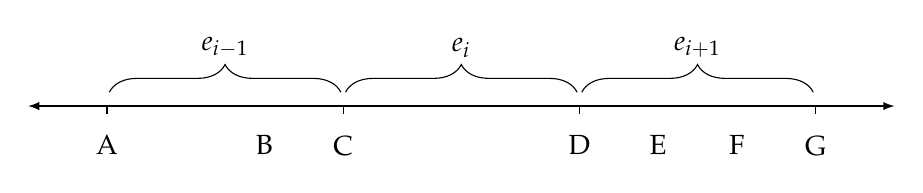
\begin{tikzpicture}
% axis
\draw[latex-latex] (0,0) -- (11,0) ;

% epoch braces
\draw [decorate,decoration={brace,amplitude=10pt} ,yshift=5pt] (1.03,0) -- (3.97,0)
  node [midway, above, yshift=9pt]{$e_{i-1}$};
\draw [decorate,decoration={brace,amplitude=10pt} ,yshift=5pt] (4.03,0) -- (6.97,0)
  node [midway, above, yshift=9pt]{$e_{i}$};
\draw [decorate,decoration={brace,amplitude=10pt} ,yshift=5pt] (7.03,0) -- (9.97,0)
  node [midway, above, yshift=9pt]{$e_{i+1}$};

% epoch boundaries
\foreach \x in  {1,4,7,10}
  \draw[shift={(\x,0)}] (0pt,0pt) -- (0pt,-3pt);

\node at (1,-0.5) {A};
\node at (3,-0.5) {B};
\node at (4,-0.5) {C};
\node at (7,-0.5) {D};
\node at (8,-0.5) {E};
\node at (9,-0.5) {F};
\node at (10,-0.5) {G};

\end{tikzpicture}

We must therefore store the last three stake distributions.
The mnemonic ``mark, set, go'' will be used to keep
track of the snapshots, where the label ``mark'' refers to the most recent snapshot,
and ``go'' refers to the snapshot that is ready to be used in the reward calculation.
In the above diagram, the snapshot taken at (A) is labeled ``mark'' during epoch $e_{i-1}$,
``set'' during epoch $e_i$ and ``go'' during epoch $e_{i+1}$. At (G) the snapshot
taken at (A) is no longer needed and will be discarded.

The two main transition systems in this section are:
\begin{itemize}
  \item The transition system named $\mathsf{EPOCH}$, which is defined in
    Section~\ref{sec:total-epoch}, covers what happens at the epoch boundary,
    such as at (A), (C), (D) and (G).
  \item The transition named $\mathsf{RUPD}$, which is defined in
    Section~\ref{sec:reward-update-trans}, covers the reward calculation that
    happens between (E) and (F).
\end{itemize}


\begin{note}
  Between time D and E we are concerned with chain growth and stability.
  Therefore this duration can be stated as 2k blocks (to state it in slots requires details about
  the particular version of the Ouroboros protocol). The duration between F and G is also 2k blocks.
  Between E and F a single honest block is enough to ensure a random nonce.
\end{note}

\subsection{Helper Functions and Accounting Fields}
\label{sec:stake-dist-helpers}

Figure~\ref{fig:funcs:epoch-helper-rewards} defines four helper functions needed
throughout the rest of the section.

\begin{itemize}
  \item The function $\fun{obligation}$ calculates the the minimal amount of coin needed to
    pay out all deposit refunds, as of the current slot.
  \item The function $\fun{poolRefunds}$ is used to calculate the total refunds
    that must be distributed for stake pools scheduled to retire.
    Note that this calculation takes a slot number corresponding to the epoch boundary slot
    when the calculation is performed.  The returned map maps pool operator hashkeys to the
    refunds, which will ultimately be returned to the registered reward account.
  \item The function $\fun{poolStake}$ filters the stake distribution to one stake pool.
\end{itemize}


%%
%% Figure - Helper Functions for Epoch Rules
%%
\begin{figure}[htb]
  \emph{Total possible refunds}
  \begin{align*}
    & \fun{obligation} \in \PParams \to \StakeCreds \to \StakePools \to \Slot \to \Coin \\
    & \obligation{pp}{stkCreds}{stpools}{cslot} =\\
    & \sum\limits_{(\_ \mapsto s) \in \var{stkCreds}}
      \refund{d_{\mathsf{val}}}{d_{\min}}{\lambda_d}{(\slotminus{cslot}{s})}
      + \sum\limits_{(\_ \mapsto s) \in \var{stpools}}
      \refund{p_{\mathsf{val}}}{p_{\min}}{\lambda_p}{(\slotminus{cslot}{s})} \\
    &
      \begin{array}{lr@{~=~}l}
        \where
          & \dval,~d_{\min},~\lambda_d
          & \fun{keyDeposit}~\var{pp},~\fun{keyMinRefund}~\var{pp},~\fun{keyDecayRate}~\var{pp}
          \\
          & p_{\mathsf{val}},~p_{\min},~\lambda_p
          & \fun{poolDeposit}~\var{pp},~\fun{poolMinRefund}~\var{pp},~\fun{poolDecayRate}~\var{pp}
      \end{array}\\
  \end{align*}
  \emph{Pool refunds}
  \begin{align*}
      & \fun{poolRefunds} \in \PParams \to (\KeyHash_{pool} \mapsto \Epoch) \to \Slot \to
      (\KeyHash_{pool} \mapsto \Coin) \\
      & \poolRefunds{pp}{retiring}{cslot} = \left\{
        \var{hk}\mapsto
          \refund{p_{\mathsf{val}}}{p_{\min}}{\lambda_p}{(\slotminus{cslot}{(\fun{slot}~e)})}
          \mid
          \var{hk}\mapsto e\in\var{retiring}
        \right\}\\
      & \where p_{\mathsf{val}},~p_{\min},~\lambda_p =
          \fun{poolDeposit}~\var{pp},~\fun{poolMinRefund}~\var{pp},~\fun{poolDecayRate}~\var{pp} \\
  \end{align*}

  \emph{Filter Stake to one Pool}
  \begin{align*}
      & \fun{poolStake} \in \KeyHash_{pool} \to (\KeyHash_{stake} \mapsto \KeyHash_{pool})
        \to \Stake \to \Stake \\
      & \poolStake{hk}{delegs}{stake} =
        \dom{(\var{delegs}\restrictrange\{hk\})\restrictdom\var{stake}}
  \end{align*}

  \caption{Helper Functions used in Rewards and Epoch Boundary}
  \label{fig:funcs:epoch-helper-rewards}
\end{figure}


The Figure~\ref{fig:defs:accounting} lists the accounting fields, denoted by $\Acnt$,
which will be used throughout this section. It consists of:
\begin{itemize}
  \item The value $\var{treasury}$ tracks the amount of coin currently stored in the treasury.
    Initially there will be no way to remove these funds.
  \item The value $\var{reserves}$ tracks the amount of coin currently stored in the reserves.
    This pot is used to pay rewards.
\end{itemize}
More will be said about the general accounting system in Section~\ref{sec:reward-calc}.

%%
%% Figure - Accounting fields
%%
\begin{figure}[htb]
  \emph{Accounting Fields}
  \begin{equation*}
    \Acnt =
    \left(
      \begin{array}{r@{~\in~}ll}
        \var{treasury} & \Coin & \text{treasury pot}\\
        \var{reserves} & \Coin & \text{reserve pot}\\
      \end{array}
    \right)
  \end{equation*}
  %
  \caption{Accounting fields}
  \label{fig:defs:accounting}
\end{figure}


\subsection{Stake Distribution Calculation}
\label{sec:stake-dist-calc}

This section defines the stake distribution calculations.
Figure~\ref{fig:epoch-defs} introduces three new derived types:
\begin{itemize}
  \item $\type{BlocksMade}$ represents the number of blocks each stake pool produced
    during an epoch.
  \item $\type{Stake}$ represents the amount of stake (in $\type{Coin}$) controlled by each
    stake pool.
\end{itemize}

%%
%% Figure - Epoch Abstract Types
%%
\begin{figure}[htb]
  \emph{Derived types}
  %
  \begin{equation*}
    \begin{array}{r@{~\in~}l@{\qquad=\qquad}lr}
      \var{blocks}
      & \BlocksMade
      & \KeyHash_{pool} \mapsto \N
      & \text{blocks made by stake pools} \\
      \var{stake}
      & \Stake
      & \Credential \mapsto \Coin
      & \text{stake} \\
    \end{array}
  \end{equation*}
  \caption{Epoch definitions}
  \label{fig:epoch-defs}
\end{figure}

The stake distribution calculation is given in Figure~\ref{fig:functions:stake-distribution}.

\begin{itemize}
\item $\fun{aggregate_{+}}$ takes a relation on $A\times B$, where $B$ is any
  monoid $(B,+,e)$ and returns a map from each $a\in A$ to the ``sum'' (using
  the monoidal $+$ operation) of all $b\in B$ such that $(a, b)\in A\times B$.
\item $\fun{stakeDistr}$ uses the $\fun{aggregate_{+}}$ function and several relations to
    compute the stake distribution, mapping each hashkey to the total coin under its control.
    Keys that are not both registered and delegated are filtered out.
    The relation passed to $\fun{aggregate_{+}}$ is made up of:
    \begin{itemize}
      \item $\fun{stakeCred_b}^{-1}$, relating credentials to (base) addresses
      \item $\left(\fun{addrPtr}\circ\var{ptr}\right)^{-1}$, relating credentials to (pointer)
        addresses
      \item $\range{utxo}$, relating addresses to coins
      \item $\fun{stakeCred_r}^{-1}\circ\var{rewards}$, relating (reward) addresses to coins
    \end{itemize}
    The notation for relations is explained in Section~\ref{sec:notation-shelley}.
\end{itemize}

%%
%% Figure Functions for Stake Distribution
%%
\begin{figure}[htb]
  \emph{Aggregation (for a monoid B)}
  %
  \begin{align*}
      & \fun{aggregate_{+}} \in \powerset{(A \times B)} \to (A\mapsto B) \\
      & \fun{aggregate_{+}}~\var{R} = \left\{a\mapsto \sum_{(a,b)\in\var{R}}b
          ~\mid~a\in\dom\var{R}\right\} \\
  \end{align*}
  %
  \emph{Stake Distribution (using functions and maps as relations)}
  %
  \begin{align*}
      & \fun{stakeDistr} \in \UTxO \to \DState \to \PState \to \Stake \\
      & \fun{stakeDistr}~{utxo}~{dstate}~{pstate} =
      (\dom{\var{activeDelegs}})\restrictdom\left(\fun{aggregate_{+}}~\var{stakeRelation}\right)\\
      & \where \\
      & ~~~~ (\var{stkCreds},~\var{rewards},~\var{delegations},~\var{ptrs},~\wcard,~\wcard)
        = \var{dstate} \\
      & ~~~~ (\var{stpools},~\wcard,~\wcard) = \var{pstate} \\
      & ~~~~ \var{stakeRelation} = \left(
        \left(\fun{stakeCred_b}^{-1}\cup\left(\fun{addrPtr}\circ\var{ptr}\right)^{-1}\right)
        \circ\left(\range{\var{utxo}}\right)
        \right)
        \cup \left(\fun{stakeCred_r}^{-1}\circ\var{rewards}\right) \\
      & ~~~~ \var{activeDelegs} =
               (\dom{stkCreds}) \restrictdom \var{delegations} \restrictrange (\dom{stpools}) \\
  \end{align*}

  \caption{Stake Distribution Function}
  \label{fig:functions:stake-distribution}
\end{figure}

\clearpage

\subsection{Snapshot Transition}
\label{sec:snapshots}

The state transition types for stake distribution snapshots are given in
Figure~\ref{fig:ts-types:snapshot}.
Each snapshot consists of:
\begin{itemize}
  \item $\var{stake}$, a stake distribution, which is defined in
    Figure~\ref{fig:epoch-defs} as a mapping of credentials to coin.
  \item $\var{delegations}$, a delegation map, mapping credentials to stake pools.
  \item $\var{poolParameters}$, storing the pool parameters of each stake pool.
\end{itemize}

The type $\type{\Snapshots}$ contains the
information needing to be saved on the epoch boundary:
\begin{itemize}
  \item $\var{pstake_{mark}}$, $\var{pstake_{set}}$ and $\var{pstake_{go}}$ are the three
    snapshots as explained in Section~\ref{sec:reward-overview}.
  \item $\var{feeSS}$ stores the fees and decayed deposit amounts at the epoch boundary.
\end{itemize}

%%
%% Figure - Snapshots Defs
%%
\begin{figure}[htb]
  \emph{Snapshot environment}
  \begin{equation*}
    \SnapshotEnv =
    \left(
      \begin{array}{r@{~\in~}ll}
        \var{pp} & \PParams & \text{protocol parameters}\\
        \var{dstate} & \DState & \text{delegation state}\\
        \var{pstate} & \PState & \text{pool state}\\
      \end{array}
    \right)
  \end{equation*}
  %
  \emph{Snapshots}
  \begin{equation*}
    \Snapshot =
    \left(
      \begin{array}{r@{~\in~}ll}
        \var{stake} & \Stake & \text{stake distribution}\\
        \var{delegations} & \Credential\mapsto\KeyHash_{pool}
                          & \text{stake delegations}\\
        \var{poolParameters} & \KeyHash_{pool} \mapsto \PoolParam & \text{pool parameters }\\
      \end{array}
    \right)
  \end{equation*}

  \begin{equation*}
    \Snapshots =
    \left(
      \begin{array}{r@{~\in~}ll}
        \var{pstake_{mark}} & \Snapshot & \text{newest stake}\\
        \var{pstake_{set}}  & \Snapshot & \text{middle stake}\\
        \var{pstake_{go}}   & \Snapshot & \text{oldest stake}\\
        \var{feeSS} & \Coin & \text{fee snapshot}\\
      \end{array}
    \right)
  \end{equation*}
  %
  \emph{Snapshot States}
  \begin{equation*}
    \SnapshotState =
    \left(
      \begin{array}{r@{~\in~}ll}
        \var{ss} & \Snapshots & \text{snapshots}\\
        \var{utxoSt} & \UTxOState & \text{utxo state}\\
      \end{array}
    \right)
  \end{equation*}
  %
  \emph{Snapshot transitions}
  \begin{equation*}
    \_ \vdash
    \var{\_} \trans{snap}{\_} \var{\_}
    \subseteq \powerset (\SnapshotEnv \times \SnapshotState \times \Epoch \times \SnapshotState)
  \end{equation*}
  %
  \caption{Snapshot transition-system types}
  \label{fig:ts-types:snapshot}
\end{figure}

The snapshot transition rule is given in Figure~\ref{fig:rules:snapshot}.
This transition has no preconditions and results in the following state change:

\begin{itemize}
  \item The oldest snapshot is replaced with the penultimate one.
  \item The penultimate snapshot is replaced with the newest one.
  \item The newest snapshot is replaced with one just calculated.
  \item The fees and decayed deposits are stored in $\var{feeSS}$. Note that this value will not
    change between epochs, unlike the $\var{fees}$ and $\var{deposits}$ values in the UTxO state.
  \item In the UTxO state, the decayed deposit amounts are moved from the deposit pot
    to the fee pool. Note that in the reward transition (Section~\ref{sec:reward-calc}),
    the value $\var{feeSS}$ will be removed from the fee pot in the UTxO state.
    The decay is calculated based on \textit{the first slot in the upcoming epoch}.
\end{itemize}

%%
%% Figure - Snapshot Rule
%%
\begin{figure}[htb]
  \begin{equation}\label{eq:snapshot}
    \inference[Snapshot]
    {
      {
      \begin{array}{r@{~\leteq~}l}
        (\var{stkCreds},~\wcard,~\var{delegations},~\wcard,~\wcard,~\wcard) & \var{dstate}\\
        (\var{stpools},~\var{poolParams},~\wcard) & \var{pstate}\\
        \var{stake} & \stakeDistr{utxo}{dstate}{pstate} \\
        \var{slot} & \firstSlot{e} \\
        \var{oblg} & \obligation{pp}{stkCreds}{stpools}{slot} \\
        \var{decayed} & \var{deposits} - \var{oblg} \\
      \end{array}
      }
    }
    {
      \begin{array}{r}
        \var{pp} \\
        \var{dstate} \\
        \var{pstate} \\
      \end{array}
      \vdash
      \left(
        \begin{array}{r}
          \var{pstake_{mark}}\\
          \var{pstake_{set}}\\
          \var{pstake_{go}}\\
          \var{feeSS} \\
          ~ \\
          \var{utxo} \\
          \var{deposits} \\
          \var{fees} \\
          \var{pup} \\
        \end{array}
      \right)
      \trans{snap}{e}
      \left(
        \begin{array}{r}
          \varUpdate{(\var{stake},~\var{delegations},~\var{poolParams})} \\
          \varUpdate{\var{pstake_{mark}}} \\
          \varUpdate{\var{pstake_{set}}} \\
          \varUpdate{\var{fees} + \var{decayed}} \\
          ~ \\
          \var{utxo} \\
          \varUpdate{\var{oblg}} \\
          \varUpdate{\var{fees} + \var{decayed}} \\
          \var{pup} \\
        \end{array}
      \right)
    }
  \end{equation}
  \caption{Snapshot Inference Rule}
  \label{fig:rules:snapshot}
\end{figure}

\clearpage

\subsection{Pool Reaping Transition}
\label{sec:pool-reap}

Figure~\ref{fig:ts-types:pool-reap} defines the types for the pool reap transition,
which is responsible for removing pools slated for retirement in the given epoch.

%%
%% Figure - Pool Reap Defs
%%
\begin{figure}[htb]
  \emph{Pool Reap State}
  \begin{equation*}
    \PlReapState =
    \left(
      \begin{array}{r@{~\in~}ll}
        \var{utxoSt} & \UTxOState & \text{utxo state}\\
        \var{acnt} & \Acnt & \text{accounting}\\
        \var{dstate} & \DState & \text{delegation state}\\
        \var{pstate} & \PState & \text{pool state}\\
      \end{array}
    \right)
  \end{equation*}
  %
  \emph{Pool Reap transitions}
  \begin{equation*}
    \_ \vdash \_ \trans{poolreap}{\_} \_ \in
    \powerset (\PParams \times \PlReapState \times \Epoch \times \PlReapState)
  \end{equation*}
  %
  \caption{Pool Reap Transition}
  \label{fig:ts-types:pool-reap}
\end{figure}


The pool-reap transition rule is given in Figure~\ref{fig:rules:pool-reap}.
This transition has no preconditions and results in the following state change:

\begin{itemize}
  \item For each retiring pool, the refund for the pool registration deposit is added to the
    pool's registered reward account, provided the reward account is still registered.
  \item The sum of all the refunds attached to unregistered reward accounts are added to the
    treasury.
  \item The deposit pool is reduced by the amount of claimed and unclaimed refunds.
  \item Any delegation to a retiring pool is removed.
  \item Each retiring pool is removed from all four maps in the pool state.
\end{itemize}

%%
%% Figure - Pool Reap Rule
%%
\begin{figure}[htb]
  \begin{equation}\label{eq:pool-reap}
    \inference[Pool-Reap]
    {
      {
      \begin{array}{r@{~\leteq~}l}
        \var{retired} & \dom{(\var{retiring}^{-1}~\var{e})} \\
        \var{pr} & \poolRefunds{pp}{(\var{retired}\restrictdom\var{stpools})}{(\firstSlot{e})} \\
        \var{rewardAcnts}
                 & \{\var{hk}\mapsto \fun{poolRAcnt}~\var{pool} \mid
                   \var{hk}\mapsto\var{pool} \in \var{retired}\restrictdom\var{poolParams} \} \\
        \var{rewardAcnts'} & \left\{
                        a \mapsto c
                        \mathrel{\Bigg|}
                        \begin{array}{r@{~\in~}l}
                          \var{hk} \mapsto c & \var{pr}, \\
                          \var{hk}\mapsto\var{a} & \var{rewardAcnts} \\
                        \end{array}
                      \right\} \\
        \var{refunds} & \dom{rewards}\restrictdom\var{rewardAcnts'} \\
        \var{mRefunds} & \dom{rewards}\subtractdom\var{rewardAcnts'} \\
        \var{refunded} & \sum\limits_{\wcard\mapsto c\in\var{refunds}} c \\
        \var{unclaimed} & \sum\limits_{\wcard\mapsto c\in\var{mRefunds}} c \\
      \end{array}
      }
    }
    {
      \var{pp}
      \vdash
      \left(
        \begin{array}{r}
          \var{utxo} \\
          \var{deposits} \\
          \var{fees} \\
          \var{ups} \\
          ~ \\
          \var{treasury} \\
          \var{reserves} \\
          ~ \\
          \var{stkCreds} \\
          \var{rewards} \\
          \var{delegations} \\
          \var{ptrs} \\
          \var{genDelegs} \\
          \var{i_{rwd}} \\
          ~ \\
          \var{stpools} \\
          \var{poolParams} \\
          \var{retiring} \\
        \end{array}
      \right)
      \trans{poolreap}{e}
      \left(
        \begin{array}{rcl}
          \var{utxo} \\
          \varUpdate{\var{deposits}}
          & \varUpdate{-}
          & \varUpdate{(\var{unclaimed} + \var{refunded})} \\
          \var{fees} \\
          \var{ups} \\
          ~ \\
          \varUpdate{\var{treasury}} & \varUpdate{+} & \varUpdate{\var{unclaimed}} \\
          \var{reserves} \\
          ~ \\
          \var{stkCreds} \\
          \varUpdate{\var{rewards}} & \varUpdate{\unionoverridePlus} & \varUpdate{\var{refunds}} \\
          \varUpdate{\var{delegations}} & \varUpdate{\subtractrange} & \varUpdate{\var{retired}} \\
          \var{ptrs} \\
          \var{genDelegs} \\
          \var{i_{rwd}}\\
          ~ \\
          \varUpdate{\var{retired}} & \varUpdate{\subtractdom} & \varUpdate{\var{stpools}} \\
          \varUpdate{\var{retired}} & \varUpdate{\subtractdom} & \varUpdate{\var{poolParams}} \\
          \varUpdate{\var{retired}} & \varUpdate{\subtractdom} & \varUpdate{\var{retiring}} \\
        \end{array}
      \right)
    }
  \end{equation}
  \caption{Pool Reap Inference Rule}
  \label{fig:rules:pool-reap}
\end{figure}

\clearpage

\subsection{Protocol Parameters Update Transition}
\label{sec:pparam-update}

Finally, reaching the epoch boundary may trigger a change in the protocol
parameters. The protocol parameters environment consists of the new
protocol parameters and the delegation and pool states.
The state change is a change of the $\UTxOState$, the $\Acnt$ states and the current $\PParams$.
The type of this state transition is given in Figure~\ref{fig:ts-types:new-proto-param}.

%%
%% Figure - New Proto Param Defs
%%
\begin{figure}[htb]
  \emph{New Proto Param environment}
  \begin{equation*}
    \NewPParamEnv =
    \left(
      \begin{array}{r@{~\in~}ll}
        \var{pp_{new}} & \PParams^? & \text{new protocol parameters}\\
        \var{dstate} & \DState & \text{delegation state}\\
        \var{pstate} & \PState & \text{pool state}\\
      \end{array}
    \right)
  \end{equation*}
  %
  \emph{New Proto Param States}
  \begin{equation*}
    \NewPParamState =
    \left(
      \begin{array}{r@{~\in~}ll}
        \var{utxoSt} & \UTxOState & \text{utxo state}\\
        \var{acnt} & \Acnt & \text{accounting}\\
        \var{pp} & \PParams & \text{current protocol parameters}\\
      \end{array}
    \right)
  \end{equation*}
  %
  \emph{New Proto Param transitions}
  \begin{equation*}
    \_ \vdash
    \var{\_} \trans{newpp}{\_} \var{\_}
    \subseteq \powerset (\NewPParamEnv \times \NewPParamState \times \Epoch \times \NewPParamState)
  \end{equation*}
  %
  \caption{New Proto Param transition-system types}
  \label{fig:ts-types:new-proto-param}
\end{figure}


Figure~\ref{fig:rules:new-proto-param} defines the new protocol parameter transition.
The transition has two rules, depending on whether or not the new protocol parameters
meet some requirements.
In particular, we require that the new parameters would not incur a debt of the system that
can not be covered by the reserves, and that the max block size is greater than the sum of the
max transaction size and the max header size.
If the requirements are met, the new protocol parameters are accepted, the proposal is reset,
and the reserves are adjusted to account for changes in the deposits.
Otherwise, the only change is that the proposal is reset.

Regarding adjusting the reserves for changes in the deposits, one of three things happens:

\begin{itemize}
  \item If the new protocol parameters mean that \textbf{fewer} funds are required in the
    deposit pot to cover all possible refunds, then the excess is moved to the reserves.

  \item If the new protocol parameters mean that \textbf{more} funds are required in the
    deposit pot to cover all possible refunds and the difference is \textbf{less} than
    the reserve pot, then funds are moved from the reserve pot to cover the difference.

  \item If the new protocol parameters mean that \textbf{more} funds are required in the
    deposit pot to cover all possible refunds and the difference is \textbf{more} than
    the reserve pot, then Rule~\ref{eq:new-pc-denied} meets the precondition and the
    only change of state is that the update proposals are reset.
\end{itemize}

Note that here, unlike most of the inference rules in this document,
the $\var{utxoSt'}$ and the $\var{acnt'}$ do not come from valid UTxO or
accounts transitions in the antecedent. We simply define the consequent
transition using these directly (instead of listing all the fields in both
states in the consequent transition). It is done this way here
for ease of reading.

%%
%% Figure - New Proto Param Rule
%%
\begin{figure}[htb]
  \begin{equation}\label{eq:new-pc-accepted}
    \hspace{-0.3cm}
    \inference[New-Proto-Param-Accept]
    {
      \var{pp_{new}}\neq\Nothing \\~\\
      {\begin{array}{rcl}
         \var{slot} & \leteq & \firstSlot{e} \\
         \var{oblg_{cur}} & \leteq & \obligation{pp}{stkCreds}{stpools}{slot} \\
         \var{oblg_{new}} & \leteq & \obligation{pp_{new}}{stkCreds}{stpools}{slot} \\
         \var{(\wcard,~\wcard,~\wcard,~\wcard,~\wcard,~\wcard,~\var{i_{rwd}})} &
                                                                                      \leteq
                              & \var{dstate}\\
         \var{diff} & \leteq & \var{oblg_{cur}} - \var{oblg_{new}}\\
         (\var{utxo},~\var{deposits},~\var{fees},~\var{ups}) & \leteq & \var{utxoSt} \\
         (\var{pup},~\var{aup},~\var{favs},~\var{avs}) & \leteq & \var{ups} \\
      \end{array}}
      \\~\\~\\
      \var{oblg_{cur}} = \var{deposits} \\
      \var{reserves} + \var{diff} \geq \sum\limits_{\wcard\mapsto\var{val}\in\var{i_{rwd}}} val \\
      \fun{maxTxSize}~\var{pp_{new}} + \fun{maxHeaderSize}~\var{pp_{new}} <
        \fun{maxBlockSize}~\var{pp_{new}}
      \\~\\
        \var{utxoSt'} \leteq
        \left(\var{utxo},~\varUpdate{oblg_{new}},~\var{fees}
        \left(\varUpdate{\emptyset},~\var{aup},~\var{favs},~\var{avs}\right)\right)
      \\~\\
      (\var{treasury},~\var{reserves})\leteq \var{acnt} \\
      \var{acnt'} \leteq (\var{treasury},~\varUpdate{reserves + diff}) \\
    }
    {
      \begin{array}{l}
        \var{pp_{new}}\\
        \var{dstate}\\
        \var{pstate}\\
      \end{array}
      \vdash
      \left(
        \begin{array}{r}
          \var{utxoSt} \\
          \var{acnt} \\
          \var{pp}
        \end{array}
      \right)
      \trans{newpp}{e}
      \left(
        \begin{array}{rcl}
          \varUpdate{utxoSt'}\\
          \varUpdate{acnt'} \\
          \varUpdate{\var{pp_{new}}} \\
        \end{array}
      \right)
    }
  \end{equation}

  \nextdef

  \begin{equation}\label{eq:new-pc-denied}
    \inference[New-Proto-Param-Denied]
    {
      \left({\begin{array}{c}
            \var{pp_{new}}=\Nothing \\
        \lor \\
        \var{reserves} + \var{diff} < \sum\limits_{\wcard\mapsto\var{val}\in\var{i_{rwd}}} val\\
        \lor \\
        \fun{maxTxSize}~\var{pp_{new}} + \fun{maxHeaderSize}~\var{pp_{new}} \geq
          \fun{maxBlockSize}~\var{pp_{new}}
      \end{array}}\right)
      \\~\\~\\
      {\begin{array}{rcl}
          \var{slot} & \leteq & \firstSlot{e} \\
          \var{oblg_{cur}} & \leteq & \obligation{pp}{stkCreds}{stpools}{slot} \\
          \var{oblg_{new}} & \leteq & \obligation{pp_{new}}{stkCreds}{stpools}{slot} \\
         \var{(\wcard,~\wcard,~\wcard,~\wcard,~\wcard,~\wcard,~\var{i_{rwd}})} &
                                                                                 \leteq
                              & \var{dstate}\\
         \var{diff} & \leteq & \var{oblg_{cur}} - \var{oblg_{new}}
      \end{array}}
      \\~\\~\\
      \left(\var{utxo},~\var{oblg},~\var{fees}
        \left(\var{pup},~\var{aup},~\var{favs},~\var{avs}\right)\right)
        \leteq \var{utxoSt} \\
        \var{utxoSt'} \leteq
        \left(\var{utxo},~\var{oblg},~\var{fees}
        \left(\varUpdate{\emptyset},~\var{aup},~\var{favs},~\var{avs}\right)\right)
    }
    {
      \begin{array}{l}
        \var{pp_{new}}\\
        \var{dstate}\\
        \var{pstate}\\
      \end{array}
      \vdash
      \left(
        \begin{array}{r}
          \var{utxoSt} \\
          \var{acnt} \\
          \var{pp}
        \end{array}
      \right)
      \trans{newpp}{e}
      \left(
        \begin{array}{rcl}
          \varUpdate{utxoSt'}\\
          \var{acnt} \\
          \var{pp}
        \end{array}
      \right)
    }
  \end{equation}
  \caption{New Proto Param Inference Rule}
  \label{fig:rules:new-proto-param}
\end{figure}

\clearpage

\subsection{Complete Epoch Boundary Transition}
\label{sec:total-epoch}

Finally, it is possible to define the complete epoch boundary transition type,
which is defined in Figure~\ref{fig:ts-types:epoch}.
The transition has no evironment.
The state is made up of the the accounting state, the snapshots, the ledger state and the
protocol parameters.
The transition uses a helper function $\fun{votedValue}$ which returns
the consensus value of update proposals in the event that consensus is met.
\textbf{Note that} $\fun{votedValue}$
\textbf{is only well-defined if } $\Quorum$
\textbf{is greater than half the number of core nodes, i.e.}
$\Quorum > |\var{genDelegs}|/2$ \textbf{.}

%%
%% Figure - Epoch Defs
%%
\begin{figure}[htb]
  \emph{Epoch States}
  \begin{equation*}
    \EpochState =
    \left(
      \begin{array}{r@{~\in~}ll}
        \var{acnt} & \Acnt & \text{accounting}\\
        \var{ss} & \Snapshots & \text{snapshots}\\
        \var{ls} & \LState & \text{ledger state}\\
        \var{prevPp} & \PParams & \text{previous protocol parameters}\\
        \var{pp} & \PParams & \text{protocol parameters}\\
      \end{array}
    \right)
  \end{equation*}
  %
  \emph{Epoch transitions}
  \begin{equation*}
    \vdash
    \var{\_} \trans{epoch}{\_} \var{\_}
    \subseteq \powerset (\EpochState \times \Epoch \times \EpochState)
  \end{equation*}
  %
  \emph{Accessor Functions}
  \begin{equation*}
    \begin{array}{r@{~\in~}lr}
      \fun{getIR} & \EpochState \to (\StakeCredential \mapsto \Coin)
                  & \text{get instantaneous rewards} \\
    \end{array}
  \end{equation*}
  %
  \emph{Helper Functions}
  \begin{align*}
      & \fun{votedValue} \in (\KeyHashGen\mapsto\PParamsUpdate) \to \PParamsUpdate^?\\
      & \fun{votedValue}~\var{vs} =
        \begin{cases}
          p & \exists p\in\range{vs}~(|vs\restrictrange p|\geq \Quorum) \\
          \Nothing & \text{otherwise} \\
        \end{cases}
  \end{align*}
  %
  \caption{Epoch transition-system types}
  \label{fig:ts-types:epoch}
\end{figure}


The epoch transition rule calls $\mathsf{SNAP}$, $\mathsf{POOLREAP}$ and $\mathsf{NEWPP}$
in sequence. It also stores the previous protocol parameters in $\var{prevPp}$.
The previous protocol parameters will be used for the reward calculation in the upcoming epoch,
note that they correspond to the epoch for which the rewards are being calculated.
Additionally, this transition also adopts the pool parameters $\var{fPoolParams}$
corresponding to the pool re-registration certificates which we submitted late in the ending epoch.
The ordering of these rules is important.
The stake pools which will be updated by $\var{fPoolParams}$ or
reaped during the $\mathsf{POOLREAP}$ transition must still be a
part of the new snapshot, and so $\mathsf{SNAP}$ must occur before these two actions.
Moreover, $\mathsf{SNAP}$ sets the deposit pot equal to current obligation,
which is a property that is preserved by $\mathsf{POOLREAP}$ and which
is necessary for the preservation of Ada property in the $ \mathsf{NEWPP}$ transition.

%%
%% Figure - Epoch Rule
%%
\begin{figure}[htb]
  \begin{equation}\label{eq:epoch}
    \inference[Epoch]
    {
      (\var{utxoSt},~(\var{dstate},~\var{pstate}))\leteq\var{ls} \\
      {
        \begin{array}{r}
          \var{pp}\\
          \var{dstate} \\
          \var{pstate} \\
        \end{array}
      }
      \vdash
      {
        \left(
          {
            \begin{array}{r}
              \var{ss} \\
              \var{utxoSt} \\
            \end{array}
          }
        \right)
      }
      \trans{\hyperref[fig:rules:snapshot]{snap}}{e}
      {
        \left(
          {
            \begin{array}{r}
              \var{ss'} \\
              \var{utxoSt'} \\
            \end{array}
          }
        \right)
      }
      \\~\\~\\
      (\var{stpools},~\var{poolParams},~\var{fPoolParams},~\var{retiring})\leteq\var{pstate}
      \\
      \var{pstate'}\leteq(\var{stpools},~\var{poolParams}\unionoverrideRight\var{fPoolParams},
      ~\emptyset,~\var{retiring})
      \\~\\~\\
      \var{pp}
      \vdash
      \left(
        {
          \begin{array}{r}
            \var{utxoSt'} \\
            \var{acnt} \\
            \var{dstate} \\
            \var{pstate'} \\
          \end{array}
        }
      \right)
      \trans{\hyperref[fig:rules:pool-reap]{poolreap}}{e}
      \left(
      {
        \begin{array}{rcl}
            \var{utxoSt''} \\
            \var{acnt'} \\
            \var{dstate'} \\
            \var{pstate''} \\
        \end{array}
      }
      \right)
      \\~\\~\\
      \var{(\wcard,~\wcard,~\wcard,~\var{pup})}\leteq\var{utxoSt'}\\
      \var{pp_{new}}\leteq\var{pp}\unionoverrideRight
      \fun{votedValue}~\var{pup}\\
      {
        \begin{array}{r}
          \var{pp_{new}}\\
          \var{dstate'}\\
          \var{pstate''}\\
        \end{array}
      }
      \vdash
      \left(
        {
          \begin{array}{r}
            \var{utxoSt''} \\
            \var{acnt'} \\
            \var{pp}\\
          \end{array}
        }
      \right)
      \trans{\hyperref[fig:rules:new-proto-param]{newpp}}{e}
      \left(
      {
        \begin{array}{rcl}
            \var{utxoSt'''} \\
            \var{acnt''} \\
            \var{pp'}\\
        \end{array}
      }
      \right)
      \\~\\~\\
      \var{ls}' \leteq (\var{utxoSt}''',~(\var{dstate}',~\var{pstate}''))
    }
    {
      \vdash
      \left(
      \begin{array}{r}
        \var{acnt} \\
        \var{ss} \\
        \var{ls} \\
        \var{prevPp} \\
        \var{pp} \\
      \end{array}
      \right)
      \trans{epoch}{e}
      \left(
      \begin{array}{rcl}
        \varUpdate{\var{acnt''}} \\
        \varUpdate{\var{ss'}} \\
        \varUpdate{\var{ls'}} \\
        \varUpdate{\var{pp}} \\
        \varUpdate{\var{pp'}} \\
      \end{array}
      \right)
    }
  \end{equation}
  \caption{Epoch Inference Rule}
  \label{fig:rules:epoch}
\end{figure}

\clearpage

\subsection{Rewards Distribution Calculation}
\label{sec:reward-dist}

This section defines the reward calculation for the proof of stake leader election.
Figure~\ref{fig:functions:rewards} defines the pool reward as described in section
5.5.2 of~\cite{delegation_design}.

\begin{itemize}
  \item The function $\fun{maxPool}$ gives the maximum reward a stake pool can receive in an epoch.
    This is a fraction of the total available rewards for the epoch.
    The result depends on the pool's relative stake, the pool's pledge and the following
    protocol parameters:
    \begin{itemize}
      \item $\var{a_0}$, the leader-stake influence
      \item $n_{opt}$, the optimal number of saturated stake pools
    \end{itemize}
  \item The function $\fun{poolReward}$ gives the total rewards available to be
    distributed to the members of the given pool. It depends on the protocol parameter $d$,
    the relative stake $\sigma$, the number $n$ of blocks the pool added to the chain and the
    total number $\overline{N}$ of blocks added to the chain in the last epoch.

\end{itemize}

%%
%% Figure - Functions for the Reward Calculation
%%
\begin{figure}[htb]
  \emph{Maximal Reward Function, called $f(s,\sigma)$ in section 5.5.2 of~\cite{delegation_design}}
  %
  \begin{align*}
      & \fun{maxPool} \in \PParams \to \Coin \to \unitInterval \to \unitInterval \to \Coin \\
      & \fun{maxPool}~\var{pp}~\var{R}~\sigma~\var{p_r} =
          ~~~\floor*{
             \frac{R}{1 + a_0}
             \cdot
             \left(
               \sigma' + p'\cdot a_0\cdot\frac{\sigma' - p'\frac{z_0-\sigma'}{z_0}}{z_0}
             \right)} \\
      & ~~~\where \\
      & ~~~~~~~a_0 = \fun{influence}~pp \\
      & ~~~~~~~n_{opt} = \fun{nopt}~pp \\
      & ~~~~~~~z_0 = 1/n_{opt} \\
      & ~~~~~~~\sigma'=\min(\sigma,~z_0) \\
      & ~~~~~~~p'=\min(p_r,~z_0) \\
  \end{align*}

  \emph{Actual Reward Function, called $\hat{f}$ in section 5.5.2 of~\cite{delegation_design}}
  %
  \begin{align*}
      & \fun{poolReward} \in \unitInterval \to \unitInterval \to \N \to \N \to \Coin \to \Coin \\
      & \poolReward{d}{\sigma}{n}{\overline{N}}{f} =
      \floor*{\overline{p}\cdot\var{f}}\\
      & ~~~\where \\
      & ~~~~~~~\overline{p} =
        \begin{cases}
          \frac{\beta}{\sigma} & \text{if } d < 0.8 \\
          1 & \text{otherwise}
        \end{cases} \\
      & ~~~~~~~\beta = \frac{n}{\max(1, \overline{N})} \\
  \end{align*}
  \caption{Functions used in the Reward Calculation}
  \label{fig:functions:rewards}
\end{figure}

\clearpage

Figure~\ref{fig:functions:reward-splitting} gives the calculation for
splitting the pool rewards with its members, as described in 6.5.2 of \cite{delegation_design}.
The portion of rewards allocated to the pool operator and owners is different
than that of the members.

\begin{itemize}
  \item The $\fun{r_{operator}}$ function calculates the leader reward, based on the pool cost,
    margin and the proportion of the pool's total stake.  Note that this reward will go to the
    reward account specified in the pool registration certificate.
  \item The $\fun{r_{member}}$ function calculates the member reward, proportionally to their
    stake after the cost and margin are removed.
\end{itemize}

%%
%% Figure - Functions for the Reward Splitting
%%
\begin{figure}[htb]
  \emph{Pool leader reward, from section 5.5.3 of \cite{delegation_design}}
  %
  \begin{align*}
      & \fun{r_{operator}} \in \Coin \to \PoolParam \to \unitInterval \to \unitIntervalNonNull \to \Coin \\
      & \lReward{\hat{f}}{pool}{s}{\sigma} =
        \begin{cases}
        \hat{f} & \hat{f} \leq c\\
        c + \floor*{(\hat{f} - c)\cdot\left(m + (1-m)\cdot\frac{s}{\sigma}\right) }&
        \text{otherwise.}
      \end{cases} \\
      & ~~~\where \\
      & ~~~~~~~c = \fun{poolCost}~pool \\
      & ~~~~~~~m = \fun{poolMargin}~pool \\
  \end{align*}

  \emph{Pool member reward, from section 5.5.3 of \cite{delegation_design}}
  %
  \begin{align*}
    & \fun{r_{member}} \in \Coin \to \PoolParam \to \unitInterval \to \unitIntervalNonNull \to \Coin \\
    & \mReward{\hat{f}}{pool}{t}{\sigma} =
      \begin{cases}
        0 & \hat{f} \leq c\\
        \floor*{(\hat{f} - c)\cdot(1-m)\cdot\frac{t}{\sigma}} &
        \text{otherwise.}
      \end{cases} \\
    & ~~~\where \\
    & ~~~~~~~c = \fun{poolCost}~pool \\
    & ~~~~~~~m = \fun{poolMargin}~pool \\
  \end{align*}

  \caption{Functions used in the Reward Splitting}
  \label{fig:functions:reward-splitting}
\end{figure}


Finally, the full reward calculation is presented in Figure~\ref{fig:functions:reward-calc}.
The calculation is done pool-by-pool.
\begin{itemize}
\item The $\fun{rewardOnePool}$ function calculates the rewards given out to
  each member of a given pool. The pool leader is identified by the stake
  credential of the pool operator. The function returns the rewards, calculated
  as follows:
    \begin{itemize}
      \item $\var{pstake}$, the total amount of stake controlled by the stake pool.
      \item $\var{ostake}$, the total amount of stake controlled by the stake pool operator
        and owners
      \item $\sigma$, the total proportion of stake controlled by the stake pool.
      \item $\overline{N}$, the expected number of blocks the pool should have produced.
      \item $\var{pledge}$, the pool's pledge in lovelace.
      \item $p_r$, the pool's pledge, as a proportion of active stake.
      \item $\var{maxP}$, maximum rewards the pool can claim if the pledge is met,
        and zero otherwise.
      \item $\var{poolR}$, the pool's actual reward, based on its performance.
      \item $\var{mRewards}$, the member's rewards as a mapping of reward accounts to coin.
      \item $\var{lReward}$, the leader's reward as coin.
      \item $\var{potentialRewards}$, the combination of $\var{mRewards}$ and $\var{lRewards}$.
      \item $\var{rewards}$, the restriction of $\var{potentialRewards}$ to the active
        reward accounts.
    \end{itemize}
  \item The $\fun{reward}$ function applies $\fun{rewardOnePool}$ to each registered stake pool.
\end{itemize}

%%
%% Figure - The Reward Calculation
%%
\begin{figure}[htb]
  \emph{Calculation to reward a single stake pool}
  %
  \begin{align*}
    & \fun{rewardOnePool} \in \PParams \to \Coin \to \N \to \N \to \KeyHash \to \PoolParam\\
      & ~~~\to \Stake \to \Coin \to \powerset{\AddrRWD}
           \to (\AddrRWD \mapsto \Coin) \\
      & \rewardOnePool{pp}{R}{n}{\overline{N}}{poolHK}{pool}{stake}{tot}{addrs_{rew}} =
          \var{rewards}\\
      & ~~~\where \\
      & ~~~~~~~\var{pstake} = \sum_{\_\mapsto c\in\var{stake}} c \\
      & ~~~~~~~\var{ostake} = \sum_{\substack{
        hk_\mapsto c\in\var{stake}\\
        hk\in(\fun{poolOwners}~\var{pool})\\
        }} c \\
      & ~~~~~~~\sigma = \var{pstake} / tot \\
      & ~~~~~~~\var{pledge} = \fun{poolPledge}~pool \\
      & ~~~~~~~p_{r} = \var{pledge} / \var{tot} \\
      & ~~~~~~~maxP =
      \begin{cases}
        \fun{maxPool}~\var{pp}~\var{R}~\sigma~\var{p_r}&
        \var{pledge} \leq \var{ostake}\\
        0 & \text{otherwise.}
      \end{cases} \\
      & ~~~~~~~\var{poolR} = \poolReward{(\fun{d}~pp)}{\sigma}{n}{\overline{N}}{maxP} \\
      & ~~~~~~~\var{mRewards} = \left\{
                                  \addrRw~hk\mapsto\mReward{poolR}{pool}{\frac{c}{tot}}{\sigma}
                                  ~\Big\vert~
                                  hk\mapsto c\in\var{stake},~~hk \neq\var{poolHK}
                               \right\}\\
      & ~~~~~~~\var{lReward} = \lReward{poolR}{pool}{\frac{\var{ostake}}{tot}}{\sigma} \\
      & ~~~~~~~\var{potentialRewards} =
                 \var{mRewards} \cup
                 \{(\fun{poolRAcnt}~\var{pool})\mapsto\var{lReward}\} \\
      & ~~~~~~~\var{rewards} = \var{addrs_{rew}}\restrictdom{\var{potentialRewards}} \\
  \end{align*}

  \emph{Calculation to reward all stake pools}
  %
  \begin{align*}
      & \fun{reward} \in \PParams \to \BlocksMade \to \Coin\to \powerset{\AddrRWD}
      \to (\KeyHash \mapsto \PoolParam) \\
      & ~~~\to \Stake \to (\KeyHash_{stake} \mapsto \KeyHash_{pool}) \to
      \Coin \to (\AddrRWD \mapsto \Coin)\\
      & \reward{pp}{blocks}{R}{addrs_{rew}}{poolParams}{stake}{delegs}{total}
          = \var{rewards}\\
      & ~~~\where \\
      & ~~~~~~~tot = \sum_{\_\mapsto c\in \var{stake}}c \\
      & ~~~~~~~\var{\overline{N}} = \sum_{\_\mapsto m\in blocks}m \\
      & ~~~~~~~pdata = \left\{
        hk\mapsto \left(p,~n,~\poolStake{hk}{delegs}{stake}\right)
        \mathrel{\Bigg|}
        \begin{array}{r@{\mapsto}c@{~\in~}l}
          hk & \var{p} & \var{poolParams} \\
          hk & \var{n} & \var{blocks} \\
        \end{array}
      \right\} \\
      & ~~~~~~~\var{results} = \left\{
        hk \mapsto \rewardOnePool{pp}{R}{n}{\overline{N}}{hk}{p}{s}{tot}{addrs_{rew}}
                 \mid
        hk\mapsto(p, n, s)\in\var{pdata} \right\} \\
      & ~~~~~~~\var{rewards} = \bigcup_{\wcard\mapsto\var{r}\in\var{results}}\var{r}
  \end{align*}
  \caption{The Reward Calculation}
  \label{fig:functions:reward-calc}
\end{figure}

\clearpage

\subsection{Reward Update Calculation}
\label{sec:reward-calc}

This section defines the calculation of a reward update.
A reward update is the information needed to account for the movement of lovelace
in the system due to paying out rewards.

Figure~\ref{fig:fund-preservation} captures the potential movement of funds in the entire system,
taking every transition system in this document into account.  Value is moved between
accounting pots, but the total amount of value in the system remains constant.
In particular, the red subgraph represents the inputs and outputs to
the ``reward pot'', a temporary variable used during the reward update calculation in
Figure~\ref{fig:functions:reward-update-creation}.
The blue arrows represent the movement of funds that pass through the ``reward pot''.


\begin{figure}[htb]
  \begin{center}
    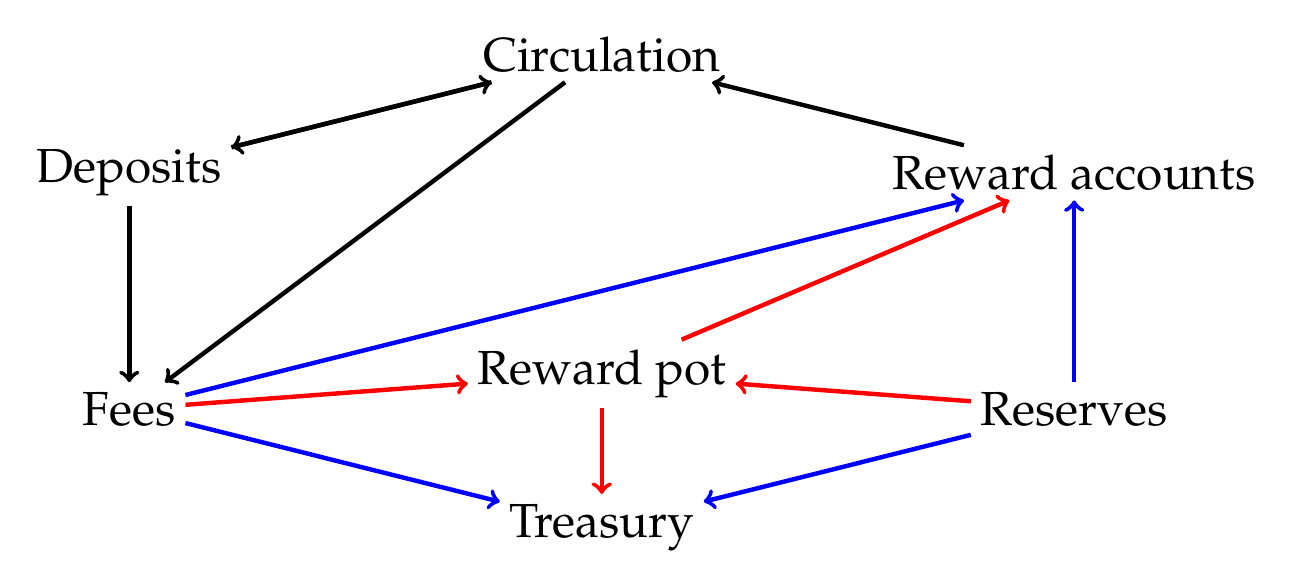
\begin{tikzpicture}
      [ x=30mm, y=30mm
      , direct/.style={black, draw}
      , implied/.style={blue, draw}
      , toTotPot/.style={red, draw}
      ]
    \node (C) at (3,2.5) {\LARGE Circulation};
    \node (R) at (5, 1) {\LARGE Reserves};
    \node (D) at (1, 2) {\LARGE Deposits};
    \node (FR) at (1,1) {\LARGE Fees};
    \node (RA) at (5, 2) {\LARGE Reward accounts};
    \node (T) at (3,0.5) {\LARGE Treasury};

    \draw[->, direct, ultra thick]
    (C) edge (D)
    (C) edge (FR)

    (D) edge (C)
    (D) edge (FR)

    (RA) edge (C);

    \draw[->, implied, ultra thick]
    (FR) edge (T)
    (FR) edge (RA)

    (R) edge (T)
    (R) edge (RA);

    \node (TP) at (3, 1.15) {\LARGE Reward pot};

    \draw[->, toTotPot, ultra thick]
    (FR) edge (TP)
    (R) edge (TP)

    (TP) edge (RA)
    (TP) edge (T);
    \end{tikzpicture}
  \end{center}
  \caption{Preservation of Value}
  \label{fig:fund-preservation}
\end{figure}

Figure~\ref{fig:defs:reward-update} defines a reward update.
It consists of four pots:
\begin{itemize}
  \item The change to the treasury. This will be a positive value.
  \item The change to the reserves. This will be a negative value.
  \item The map of new individual rewards (to be added to the existing rewards).
  \item The change to the fee pot. This will be a negative value.
    rewards.
\end{itemize}

%%
%% Figure - Reward Update Defs
%%
\begin{figure}[htb]
  \emph{Reward Update}
  \begin{equation*}
    \RewardUpdate =
    \left(
      \begin{array}{r@{~\in~}ll}
        \Delta t & \Coin & \text{change to the treasury} \\
        \Delta r & \Coin & \text{change to the reserves} \\
        \var{rs} & \AddrRWD\mapsto\Coin & \text{new individual rewards} \\
        \Delta f & \Coin & \text{change to the fee pot} \\
      \end{array}
    \right)
  \end{equation*}
  %
  \caption{Rewards Update type}
  \label{fig:defs:reward-update}
\end{figure}

\clearpage

Figure~\ref{fig:functions:reward-update-creation} defines two functions,
$\fun{createRUpd}$ to create a reward update and $\fun{applyRUpd}$ to apply a
reward update to an instance of $\EpochState$.

The $\fun{createRUpd}$ function does the following:
\begin{itemize}
  \item Note that for all the calculations below, we use the previous protocol parameters
    $\var{prevPp}$, which corresponds to the parameters during the epoch for which we
    are creating rewards.
  \item First we calculate the change to the reserves,
    as determined by the $\rho$ protocol parameter.
  \item Next we calculate $\var{rewardPot}$, the total amount of coin available for rewards this
    epoch, as described in section 6.4 of \cite{delegation_design}. It consists of four pots:
    \begin{itemize}
      \item The fee pot, containing the transaction fees from the epoch.
      \item The amount of coin in the deposit pot that is no longer needed, due to decay.
      \item The amount of monetary expansion from the reserves, calculated above.
    \end{itemize}
    Note that the fee pot and the decayed amount are taken from the snapshot taken at the
    epoch boundary.  (See~Figure\ref{fig:rules:snapshot}).
  \item Next we calculate the proportion of the reward pot that will move to the treasury,
    as determined by the $\tau$ protocol parameter. The remaining pot is called the
    $\var{R}$, just as in section 6.5 of \cite{delegation_design}.
  \item The rewards are calculated, using the oldest stake distribution snapshot (the one
    labeled ``go'').
    As given by $\fun{maxPool}$, each pool can receive a maximal amount, determined by its
    performance.  The difference between the maximal amount and the actual amount received is
    added to the amount moved to the treasury.
  \item The fee pot will be reduced by $\var{feeSS}$.
\end{itemize}

Note that fees are not explicitly removed from any account:
the fees come from transactions paying them and are accounted for whenever
transactions are processed and when the deposit decay value comes from returning
smaller refunds for deposits than were paid upon depositing.

The $\fun{applyRUpd}$ function does the following:
    \begin{itemize}
      \item Adjust the treasury, reserves and fee pots by the appropriate amounts.
      \item Add each individual reward to the global reward mapping.
    \end{itemize}

These two functions will be used in the blockchain transition systems in Section~\ref{sec:chain}.
In particular,
$\fun{createRUpd}$ will be used in Equation~\ref{eq:reward-update},
and $\fun{applyRUpd}$ will be used in Equation~\ref{eq:new-epoch}.

%%
%% Figure - The Reward Update Creation
%%
\begin{figure}[htb]
  \emph{Calculation to create a reward update}
  %
  \begin{align*}
    & \fun{createRUpd} \in \BlocksMade \to \EpochState \to \Coin \to \RewardUpdate \\
    & \createRUpd{b}{es}{total} = \left(
      \Delta t_1+\Delta t_2,-~\Delta r,~\var{rs},~-\var{feeSS}\right) \\
    & ~~~\where \\
    & ~~~~~~~(\var{acnt},~\var{ss},~\var{ls},~\var{prevPp},~\wcard) = \var{es} \\
    & ~~~~~~~(\wcard,~\wcard,~\var{pstake_{go}},~\var{poolsSS},~\var{feeSS}) = \var{ss}\\
    & ~~~~~~~(\var{stake},~\var{delegs}) = \var{pstate_{go}} \\
    & ~~~~~~~(\wcard,~\var{reserves}) = \var{acnt} \\
    & ~~~~~~~\left(
      \wcard,~
      \left(
      \left(\wcard,~\var{rewards},~\wcard,~\wcard,~\wcard,~\wcard\right)~
      \wcard
      \right)
      \right) = \var{ls} \\
    & ~~~~~~~\Delta r = \floor*{\min(1,\eta) \cdot (\fun{rho}~\var{prevPp}) \cdot
      \var{reserves}}
    \\
    & ~~~~~~~\eta = \frac{blocksMade}{\SlotsPerEpoch \cdot \ActiveSlotCoeff} \\
    & ~~~~~~~\var{rewardPot} = \var{feeSS} + \Delta r \\
    & ~~~~~~~\Delta t_1 = \floor*{(\fun{tau}~\var{prevPp}) \cdot \var{rewardPot}} \\
    & ~~~~~~~\var{R} = \var{rewardPot} - \Delta t_1 \\
    & ~~~~~~~\var{circulation} = \var{total} - \var{reserves} \\
    & ~~~~~~~\var{rs}
      = \reward{prevPp}{b}{R}{(\dom{rewards})}{poolsSS}{stake}{delegs}{circulation} \\
    & ~~~~~~~\Delta t_{2} = R - \left(\sum\limits_{\_\mapsto c\in\var{rs}}c\right) \\
    & ~~~~~~~blocksMade = \sum_{\wcard \mapsto m \in b}m
  \end{align*}

  \caption{Reward Update Creation}
  \label{fig:functions:reward-update-creation}
\end{figure}

\begin{figure}[htb]
  \emph{Applying a reward update}
  %
  \begin{align*}
      & \fun{applyRUpd} \in \RewardUpdate \to \EpochState \to \EpochState \\
      & \fun{applyRUpd}~
      \left(
        \begin{array}{c}
          \Delta t \\
          \Delta r \\
          \var{rs} \\
          \Delta f \\
        \end{array}
    \right)
      \left(
        \begin{array}{c}
          \var{treasury} \\
          \var{reserves} \\
          ~ \\
          \var{stkCreds} \\
          \var{rewards} \\
          \var{delegations} \\
          \var{ptrs} \\
          \var{genDelegs} \\
          \var{i_{rwd}}
          \\~ \\
          \var{stpools} \\
          \var{poolParams} \\
          \var{retiring} \\
          ~ \\
          \var{utxo} \\
          \var{deposits} \\
          \var{fees} \\
          \var{up} \\
          ~ \\
          \var{prevPp} \\
          \var{pp} \\
        \end{array}
      \right)
      =
      \left(
        \begin{array}{c}
          \varUpdate{\var{treasury} + \Delta t}\\
          \varUpdate{\var{reserves} + \Delta r}\\
          ~ \\
          \var{\var{stkCreds}} \\
          \varUpdate{\var{rewards}\unionoverridePlus\var{rs}} \\
          \var{delegations} \\
          \var{ptrs} \\
          \var{genDelegs} \\
          \var{i_{rwd}}
          \\~ \\
          \var{stpools} \\
          \var{poolParams} \\
          \var{retiring} \\
          ~ \\
          \var{utxo} \\
          \var{deposits} \\
          \varUpdate{\var{fees}+\Delta f} \\
          \var{up} \\
          ~ \\
          \var{prevPp} \\
          \var{pp} \\
        \end{array}
    \right)
  \end{align*}

  \caption{Reward Update Application}
  \label{fig:functions:reward-update-application}
\end{figure}

\clearpage


\clearpage

\section{Properties}
\label{sec:properties}
\section{Formal Properties}
\label{sec:properties}

This appendix collects the main formal properties that the new ledger rules are expected to satisfy.

\begin{enumerate}[label=P{\arabic*}:\ ]
\item
  \emph{Consistency with Shelley.}
  All formal properties that were defined for Shelley in \ref{XX} remain valid.\todo{Confirm this, or list any exceptions.}
\item
  \emph{Consistency with Multi-Asset.}
  All formal properties that were defined for multi-asset tokens in \ref{XX} also remain valid.\todo{Confirm this, or list any exceptions.}
\item
  \emph{Ada Consistency.}
  Any token with the $\PolicyID$ of Ada is an Ada token, i.e. it
  also has the $\AssetID$ of Ada.
\item
  \emph{General Accounting.}
  The \emph{general accounting} property\todo{Reference or explain this} holds for any transaction,
  whether it is fully processed or just paying fees. In particular,
  this implies that the total amount of Ada in the system is constant.
\item
  \emph{Fee Movement.}
  If a transaction is accepted and marked as paying fees only
  (i.e. $\fun{txvaltag}\, tx = \True$), then the only change to the ledger
  when processing the transaction is that the inputs marked for paying
  fees are moved to the fee pot.
\item
  \emph{Transaction Validation.}
  If a Shelley transaction is accepted, it is fully processed.\todo{What does this mean? Is this: Transaction consistency - any transaction that is successfully validated can be executed successfully by the interpreter.}
\item
  \emph{Extended UTxO Validation.}
  If a transaction extends the UTxO, all its scripts validate, and
  if it has a script that does not validate, it cannot extend the
  UTxO.
\item
  \emph{Non-Token Forging.}
  A valid transaction that does not forge tokens satisfies the
  accounting property of the Shelley ledger where the type $\Coin$ is
  replaced by $\Value$.
\item
  \todo{\emph{Script consistency.} Scripts are only processed by valid version of the interpreter.}
\item
  \todo{\emph{Backwards compatibility.} All scripts that could be processed by any previous version of the interpreter
    remain valid indefinitely.}
\item
  \todo{\emph{Cost consistency.} - no transaction exceeds the specified resource bounds.}
\item
  \todo{\emph{Backwards Compatibility.} Any transaction that was accepted in a previous version of the ledger rules
    has exactly the same cost and effect, except that the transaction output is extended.}
\item
  ... \todo{Anything else?}
\end{enumerate}


\clearpage

\section{Non-Integral Calculations}
\label{sec:non-integr-calc}
In the ledger there are several cases where non-integral calculations are
required. This does concern the delegation transitions, not value transactions.

\subsection{Types of Non-Integral Calculations}
\label{sec:types-non-integral}

The specification employs non-integral calculations for different mathematical
operations. Table~\ref{tab:func-non-integral} shows the function and transition
rules that use non-integral calculations and which type.

\begin{table}[ht]
  \centering
  \begin{tabular}{lccccc}
    \toprule
    name & page & multiplication & division & exponential function & exponentiation \\
    \midrule
    \fun{refund}
         & \pageref{fig:functions:deposits-refunds} & \checkmark & & \checkmark & \\
    \fun{maxPool}
         & \pageref{fig:functions:rewards} & \checkmark & \checkmark & & \\
    \fun{movingAvg}
         & \pageref{fig:functions:rewards} & \checkmark & \checkmark && \\
    \fun{poolReward}
         & \pageref{fig:functions:rewards} & \checkmark & & \checkmark &
                                                                         \checkmark \\
    \fun{r_{leader}}
         & \pageref{fig:functions:reward-splitting} & \checkmark & \checkmark &&\\
    \fun{mReward}
         & \pageref{fig:functions:reward-splitting} & \checkmark & \checkmark
                                            &&\\
    \fun{rewardOnePool}
         & \pageref{fig:functions:reward-calc} & \checkmark & \checkmark && \\
    \fun{updateAvgs}
         & \pageref{fig:functions:epoch} & \checkmark & \checkmark &&\\
    \fun{ACCNT}
         &\pageref{fig:rules:accnt} & \checkmark &&& \\
    \bottomrule
  \end{tabular}
  \caption{Functions with Non-Integral Calculation}
  \label{tab:func-non-integral}
\end{table}

The transcendental exponential function is used in reward and refund calculation
to model the decay of the deposit values. The pool reward uses exponentiation to
calculate a pool's ranking.

The domain for the exponential function are the non-negative reals, more
precisely the distribution parameter $\lambda \in (0, \infty)$ multiplied by a
discrete non-negative duration $\delta$.

The domain of the base of the exponentiation in $\fun{poolReward}$ are the
non-negative reals resulting from the calculation in $\fun{movingAvg}$, the
exponent $\gamma$ is a constant take from the protocol parameters.

\subsection{Implementation of Non-Integer Calculations}
\label{sec:impl-non-integ}

The large part consists of multiplication and division which can easily be done
using fractional arithmetic to the desired precision. The precision necessary is
bounded by the ability to represent a single lovelace in all calculations.

\subsubsection{Function Simplification}
\label{sec:funct-simpl}

The transcendental function $e^{x}$ can be approximated using different
approaches, depending on the desired accuracy. In general, one uses the
exponential laws $e^{x} = 1/e^{-x}$ and
$e^{x} = \left(e^{\frac{x}{n}} \right)^{n}, n \in \mathbb{N}$ to reduce the
approximation to the unit interval and apply fast integral exponentiation
afterwards.

Exponentiation is implemented using the law
$a^{b} = e^{\ln(a^{b})}= e^{b\ln(a)}$. This therefore requires being able to
calculate $e^{x}$ and $\ln(x)$. The approximation of the natural logarithm can
be approximated using different approaches, again, depending on the desired
accuracy. Most approximations work for $\ln(x), x \in [1, c)$ with some $c >
0$. One then uses the law $\log_{b}(x) = \log_{b}(\frac{x}{b^{n}}b^{n})$ where
$n \in \mathbb{N}$ is chosen in such a way that $\frac{x}{b^{n}} \in [1,
c)$. Using this, one can separate the calculation of the integral and decimal
part as follows:

\begin{equation*}
  \log_{b}(\frac{x}{b^{n}}b^{n})=\log_{b}(b^{n}) + \log_{b}(\frac{x}{b^{n}})=
  n + \log(\frac{x}{b^{n}})
\end{equation*}

%%% Local Variables:
%%% mode: latex
%%% TeX-master: "ledger-spec"
%%% End:


\newpage

\begin{appendix}
  \section{Proofs}
\label{sec:proofs}

\newif\ifproofs
% \proofstrue comment in to include generated proofs

For the proofs we use the automated theorem prover
MetiTarski~\cite{DBLP:journals/jar/AkbarpourP10} which is specialized for proofs
over real arithmetic, including elementary functions.

\begin{proof}
The property~(\ref{prop:minimal-refund}) (p.~\pageref{prop:minimal-refund}) for
the minimal refund can be proven automatically via

\begin{verbatim}
fof(minimal_refund, conjecture,
! [Dmin, Lambda, Delta, Dval] :
((Dmin : (=0,1=) & Lambda > 0 & Delta > 0 & Dval > 0
=>
Dval*Dmin >= 0 &
(Dval * (Dmin + (1 - Dmin) * exp(-Lambda * Delta))) : (=Dval * Dmin, Dval=)))).

fof(floor_lower_upper, conjecture,
! [X] :
(X >= 0 => X - 1 <= floor(X) & floor(X) <= X)).
\end{verbatim}
  \verb|minimal_refund| shows that the resulting value is within the interval
  $[d_{val}\cdot d_{min}, d_{val}]$ and that $d_{val}\cdot d_{min}$ is
  non-negative, while \verb|floor_lower_upper| shows that the floor of a value
  $x$ has an upper bound $x$ and lower bound $x - 1$.

\ifproofs
\begin{verbatim}
SZS output start CNFRefutation for minRefund.tptp
cnf(lgen_le_neg, axiom, (X <= Y | ~ lgen(0, X, Y))).

cnf(leq_left_divide_mul_pos, axiom, (Y * Z < X | X / Z <= Y | Z <= 0)).

cnf(interval_intro, axiom,
    (~ lgen(R, A, X) | ~ lgen(S, X, B) | interval(R, A, S, B, X))).

cnf(interval_elim1, axiom, (~ interval(R, A, S, B, X) | lgen(R, A, X))).

cnf(interval_elim2, axiom, (~ interval(R, A, S, B, X) | lgen(S, X, B))).

cnf(exp_upper_bound_cf2, axiom,
    (0 <= X | ~ lgen(R, (X ^ 2 + 6 * X + 12) / (X ^ 2 - 6 * X + 12), Y) |
     lgen(R, exp(X), Y))).

fof(minimal_refund, conjecture,
    (! [Dmin, Lambda, Delta, Dval] :
       ((interval(0, 0, 0, 1, Dmin) & 0 < Lambda & 0 < Delta & 0 < Dval) =>
        (0 <= Dval * Dmin &
         interval(0, Dval * Dmin, 0, Dval,
                  Dval * (Dmin + (1 - Dmin) * exp(-Lambda * Delta))))))).

fof(subgoal_0, plain,
    (! [Dmin, Lambda, Delta, Dval] :
       ((interval(0, 0, 0, 1, Dmin) & 0 < Lambda & 0 < Delta & 0 < Dval) =>
        0 <= Dval * Dmin)), inference(strip, [], [minimal_refund])).

fof(subgoal_1, plain,
    (! [Dmin, Lambda, Delta, Dval] :
       (((interval(0, 0, 0, 1, Dmin) & 0 < Lambda & 0 < Delta & 0 < Dval) &
         0 <= Dval * Dmin) =>
        interval(0, Dval * Dmin, 0, Dval,
                 Dval * (Dmin + (1 - Dmin) * exp(-Lambda * Delta))))),
    inference(strip, [], [minimal_refund])).

fof(negate_0_0, plain,
    (~ ! [Dmin, Lambda, Delta, Dval] :
         ((interval(0, 0, 0, 1, Dmin) & 0 < Lambda & 0 < Delta &
           0 < Dval) => 0 <= Dval * Dmin)),
    inference(negate, [], [subgoal_0])).

fof(normalize_0_0, plain,
    (? [Delta, Dmin, Dval, Lambda] :
       (0 < Delta & 0 < Dval & 0 < Lambda & Dval * Dmin < 0 &
        interval(0, 0, 0, 1, Dmin))),
    inference(canonicalize, [], [negate_0_0])).

fof(normalize_0_1, plain,
    (skoDvalC2 * skoDminC2 < 0 & 0 < skoDeltaC2 & 0 < skoDvalC2 &
     0 < skoLambdaC2 & interval(0, 0, 0, 1, skoDminC2)),
    inference(skolemize, [], [normalize_0_0])).

fof(normalize_0_2, plain, (interval(0, 0, 0, 1, skoDminC2)),
    inference(conjunct, [], [normalize_0_1])).

fof(normalize_0_3, plain, (skoDvalC2 * skoDminC2 < 0),
    inference(conjunct, [], [normalize_0_1])).

fof(normalize_0_4, plain, (0 < skoLambdaC2),
    inference(conjunct, [], [normalize_0_1])).

fof(normalize_0_5, plain, (0 < skoDvalC2),
    inference(conjunct, [], [normalize_0_1])).

fof(normalize_0_6, plain, (0 < skoDeltaC2),
    inference(conjunct, [], [normalize_0_1])).

cnf(refute_0_0, plain, (interval(0, 0, 0, 1, skoDminC2)),
    inference(canonicalize, [], [normalize_0_2])).

cnf(refute_0_1, plain,
    (~ interval(0, 0, 0, 1, skoDminC2) | lgen(0, 0, skoDminC2)),
    inference(subst, [], [interval_elim1])).

cnf(refute_0_2, plain, (lgen(0, 0, skoDminC2)),
    inference(resolve, [], [refute_0_0, refute_0_1])).

cnf(refute_0_3, plain, (0 <= skoDminC2),
    inference(arithmetic, [], [refute_0_2])).

cnf(refute_0_4, plain, (skoDvalC2 * skoDminC2 < 0),
    inference(canonicalize, [], [normalize_0_3])).

cnf(refute_0_5, plain, (0 < skoDvalC2 * (skoDminC2 * -1)),
    inference(arithmetic, [], [refute_0_4])).

cnf(refute_0_6, plain, (0 < skoLambdaC2),
    inference(canonicalize, [], [normalize_0_4])).

cnf(refute_0_7, plain, (0 < skoDvalC2),
    inference(canonicalize, [], [normalize_0_5])).

cnf(refute_0_8, plain, (0 < skoDeltaC2),
    inference(canonicalize, [], [normalize_0_6])).

cnf(refute_0_9, plain, (skoDminC2 < 0),
    inference(decision, [],
              [refute_0_5, refute_0_6, refute_0_7, refute_0_8])).

cnf(refute_0_10, plain, ($false),
    inference(resolve, [], [refute_0_3, refute_0_9])).

fof(negate_1_0, plain,
    (~ ! [Dmin, Lambda, Delta, Dval] :
         (((interval(0, 0, 0, 1, Dmin) & 0 < Lambda & 0 < Delta &
            0 < Dval) & 0 <= Dval * Dmin) =>
          interval(0, Dval * Dmin, 0, Dval,
                   Dval * (Dmin + (1 - Dmin) * exp(-Lambda * Delta))))),
    inference(negate, [], [subgoal_1])).

fof(normalize_1_0, plain,
    (? [Delta, Dmin, Dval, Lambda] :
       (0 < Delta & 0 < Dval & 0 < Lambda &
        ~ interval(0, Dval * Dmin, 0, Dval,
                   Dval * (Dmin + (1 - Dmin) * exp(-Lambda * Delta))) &
        0 <= Dval * Dmin & interval(0, 0, 0, 1, Dmin))),
    inference(canonicalize, [], [negate_1_0])).

fof(normalize_1_1, plain,
    (0 < skoDeltaC3 & 0 < skoDvalC3 & 0 < skoLambdaC3 &
     ~ interval(0, skoDvalC3 * skoDminC3, 0, skoDvalC3,
                skoDvalC3 *
                (skoDminC3 +
                 (1 - skoDminC3) * exp(-skoLambdaC3 * skoDeltaC3))) &
     0 <= skoDvalC3 * skoDminC3 & interval(0, 0, 0, 1, skoDminC3)),
    inference(skolemize, [], [normalize_1_0])).

fof(normalize_1_2, plain,
    (~ interval(0, skoDvalC3 * skoDminC3, 0, skoDvalC3,
                skoDvalC3 *
                (skoDminC3 +
                 (1 - skoDminC3) * exp(-skoLambdaC3 * skoDeltaC3)))),
    inference(conjunct, [], [normalize_1_1])).

fof(normalize_1_3, plain, (interval(0, 0, 0, 1, skoDminC3)),
    inference(conjunct, [], [normalize_1_1])).

fof(normalize_1_4, plain, (0 <= skoDvalC3 * skoDminC3),
    inference(conjunct, [], [normalize_1_1])).

fof(normalize_1_5, plain, (0 < skoLambdaC3),
    inference(conjunct, [], [normalize_1_1])).

fof(normalize_1_6, plain, (0 < skoDvalC3),
    inference(conjunct, [], [normalize_1_1])).

fof(normalize_1_7, plain, (0 < skoDeltaC3),
    inference(conjunct, [], [normalize_1_1])).

cnf(refute_1_0, plain,
    (1 *
     (12 +
      skoLambdaC3 *
      (skoDeltaC3 * 6 + skoLambdaC3 * (skoDeltaC3 * skoDeltaC3))) <
     12 +
     skoLambdaC3 *
     (skoDeltaC3 * -6 + skoLambdaC3 * (skoDeltaC3 * skoDeltaC3)) |
     12 +
     skoLambdaC3 *
     (skoDeltaC3 * 6 + skoLambdaC3 * (skoDeltaC3 * skoDeltaC3)) <= 0 |
     (12 +
      skoLambdaC3 *
      (skoDeltaC3 * -6 + skoLambdaC3 * (skoDeltaC3 * skoDeltaC3))) /
     (12 +
      skoLambdaC3 *
      (skoDeltaC3 * 6 + skoLambdaC3 * (skoDeltaC3 * skoDeltaC3))) <= 1),
    inference(subst, [], [leq_left_divide_mul_pos])).

cnf(refute_1_1, plain,
    (~ lgen(0, exp(X_000190), X_000191) | exp(X_000190) <= X_000191),
    inference(subst, [], [lgen_le_neg])).

cnf(refute_1_2, plain,
    (~ lgen(0,
            (X_000190 ^ 2 + 6 * X_000190 + 12) /
            (X_000190 ^ 2 - 6 * X_000190 + 12), X_000191) | 0 <= X_000190 |
     lgen(0, exp(X_000190), X_000191)),
    inference(subst, [], [exp_upper_bound_cf2])).

cnf(refute_1_3, plain,
    (~ lgen(0,
            (X_000190 ^ 2 + 6 * X_000190 + 12) /
            (X_000190 ^ 2 - 6 * X_000190 + 12), X_000191) | 0 <= X_000190 |
     exp(X_000190) <= X_000191),
    inference(resolve, [], [refute_1_2, refute_1_1])).

cnf(refute_1_4, plain,
    (X_000191 <
     (12 + X_000190 * (6 + X_000190)) / (12 + X_000190 * (-6 + X_000190)) |
     0 <= X_000190 | exp(X_000190) <= X_000191),
    inference(arithmetic, [], [refute_1_3])).

cnf(refute_1_5, plain,
    (1 <
     (12 +
      skoLambdaC3 * (skoDeltaC3 * -1) *
      (6 + skoLambdaC3 * (skoDeltaC3 * -1))) /
     (12 +
      skoLambdaC3 * (skoDeltaC3 * -1) *
      (-6 + skoLambdaC3 * (skoDeltaC3 * -1))) |
     0 <= skoLambdaC3 * (skoDeltaC3 * -1) |
     exp(skoLambdaC3 * (skoDeltaC3 * -1)) <= 1),
    inference(subst, [], [refute_1_4])).

cnf(refute_1_6, plain,
    (~ interval(0, skoDvalC3 * skoDminC3, 0, skoDvalC3,
                skoDvalC3 *
                (skoDminC3 +
                 (1 - skoDminC3) * exp(-skoLambdaC3 * skoDeltaC3)))),
    inference(canonicalize, [], [normalize_1_2])).

cnf(refute_1_7, plain,
    (~ interval(0, skoDvalC3 * skoDminC3, 0, skoDvalC3,
                skoDvalC3 * skoDminC3 +
                exp(skoLambdaC3 * (skoDeltaC3 * -1)) *
                (skoDvalC3 * (1 + skoDminC3 * -1)))),
    inference(arithmetic, [], [refute_1_6])).

cnf(refute_1_8, plain,
    (~ lgen(0, skoDvalC3 * skoDminC3,
            skoDvalC3 * skoDminC3 +
            exp(skoLambdaC3 * (skoDeltaC3 * -1)) *
            (skoDvalC3 * (1 + skoDminC3 * -1))) |
     ~ lgen(0,
            skoDvalC3 * skoDminC3 +
            exp(skoLambdaC3 * (skoDeltaC3 * -1)) *
            (skoDvalC3 * (1 + skoDminC3 * -1)), skoDvalC3) |
     interval(0, skoDvalC3 * skoDminC3, 0, skoDvalC3,
              skoDvalC3 * skoDminC3 +
              exp(skoLambdaC3 * (skoDeltaC3 * -1)) *
              (skoDvalC3 * (1 + skoDminC3 * -1)))),
    inference(subst, [], [interval_intro])).

cnf(refute_1_9, plain,
    (~ lgen(0, skoDvalC3 * skoDminC3,
            skoDvalC3 * skoDminC3 +
            exp(skoLambdaC3 * (skoDeltaC3 * -1)) *
            (skoDvalC3 * (1 + skoDminC3 * -1))) |
     ~ lgen(0,
            skoDvalC3 * skoDminC3 +
            exp(skoLambdaC3 * (skoDeltaC3 * -1)) *
            (skoDvalC3 * (1 + skoDminC3 * -1)), skoDvalC3)),
    inference(resolve, [], [refute_1_8, refute_1_7])).

cnf(refute_1_10, plain,
    (0 <
     exp(skoLambdaC3 * (skoDeltaC3 * -1)) *
     (skoDvalC3 * (-1 + skoDminC3)) |
     skoDvalC3 * (1 + skoDminC3 * -1) <
     exp(skoLambdaC3 * (skoDeltaC3 * -1)) *
     (skoDvalC3 * (1 + skoDminC3 * -1))),
    inference(arithmetic, [], [refute_1_9])).

cnf(refute_1_11, plain,
    (0 <
     exp(skoLambdaC3 * (skoDeltaC3 * -1)) *
     (skoDvalC3 * (-1 + skoDminC3)) |
     exp(skoLambdaC3 * (skoDeltaC3 * -1)) *
     (skoDvalC3 * (-1 + skoDminC3)) <= 0),
    introduced(tautology, [assume])).

cnf(refute_1_12, plain,
    (0 < 0 | skoDvalC3 * (-1 + skoDminC3) < 0 |
     0 < skoDvalC3 * (-1 + skoDminC3) |
     exp(skoLambdaC3 * (skoDeltaC3 * -1)) *
     (skoDvalC3 * (-1 + skoDminC3)) <= 0),
    inference(split, [], [refute_1_11])).

cnf(refute_1_13, plain,
    (0 < skoDvalC3 * (-1 + skoDminC3) |
     0 < skoDvalC3 * (1 + skoDminC3 * -1) |
     exp(skoLambdaC3 * (skoDeltaC3 * -1)) *
     (skoDvalC3 * (-1 + skoDminC3)) <= 0),
    inference(arithmetic, [], [refute_1_12])).

cnf(refute_1_14, plain,
    (exp(skoLambdaC3 * (skoDeltaC3 * -1)) <
     0 / (skoDvalC3 * (-1 + skoDminC3)) |
     0 <= skoDvalC3 * (-1 + skoDminC3) |
     exp(skoLambdaC3 * (skoDeltaC3 * -1)) *
     (skoDvalC3 * (-1 + skoDminC3)) <= 0),
    inference(split, [], [refute_1_11])).

cnf(refute_1_15, plain,
    (exp(skoLambdaC3 * (skoDeltaC3 * -1)) *
     (skoDvalC3 * (-1 + skoDminC3)) <= 0 |
     skoDvalC3 * (1 + skoDminC3 * -1) <= 0),
    inference(arithmetic, [], [refute_1_14])).

cnf(refute_1_16, plain,
    (0 < skoDvalC3 * (-1 + skoDminC3) |
     exp(skoLambdaC3 * (skoDeltaC3 * -1)) *
     (skoDvalC3 * (-1 + skoDminC3)) <= 0),
    inference(resolve, [], [refute_1_15, refute_1_13])).

cnf(refute_1_17, plain, (interval(0, 0, 0, 1, skoDminC3)),
    inference(canonicalize, [], [normalize_1_3])).

cnf(refute_1_18, plain,
    (~ interval(0, 0, 0, 1, skoDminC3) | lgen(0, skoDminC3, 1)),
    inference(subst, [], [interval_elim2])).

cnf(refute_1_19, plain, (lgen(0, skoDminC3, 1)),
    inference(resolve, [], [refute_1_17, refute_1_18])).

cnf(refute_1_20, plain, (skoDminC3 <= 1),
    inference(arithmetic, [], [refute_1_19])).

cnf(refute_1_21, plain, (0 <= skoDvalC3 * skoDminC3),
    inference(canonicalize, [], [normalize_1_4])).

cnf(refute_1_22, plain, (skoDvalC3 * (skoDminC3 * -1) <= 0),
    inference(arithmetic, [], [refute_1_21])).

cnf(refute_1_23, plain, (0 < skoLambdaC3),
    inference(canonicalize, [], [normalize_1_5])).

cnf(refute_1_24, plain, (0 < skoDvalC3),
    inference(canonicalize, [], [normalize_1_6])).

cnf(refute_1_25, plain, (0 < skoDeltaC3),
    inference(canonicalize, [], [normalize_1_7])).

cnf(refute_1_26, plain, (skoDvalC3 * (-1 + skoDminC3) <= 0),
    inference(decision, [],
              [refute_1_20, refute_1_22, refute_1_23, refute_1_24,
               refute_1_25])).

cnf(refute_1_27, plain,
    (exp(skoLambdaC3 * (skoDeltaC3 * -1)) *
     (skoDvalC3 * (-1 + skoDminC3)) <= 0),
    inference(resolve, [], [refute_1_26, refute_1_16])).

cnf(refute_1_28, plain,
    (skoDvalC3 * (1 + skoDminC3 * -1) <
     exp(skoLambdaC3 * (skoDeltaC3 * -1)) *
     (skoDvalC3 * (1 + skoDminC3 * -1))),
    inference(resolve, [], [refute_1_27, refute_1_10])).

cnf(refute_1_29, plain,
    (skoDvalC3 * (1 + skoDminC3 * -1) /
     (skoDvalC3 * (1 + skoDminC3 * -1)) <
     exp(skoLambdaC3 * (skoDeltaC3 * -1)) |
     skoDvalC3 * (1 + skoDminC3 * -1) <= 0),
    inference(split, [], [refute_1_28])).

cnf(refute_1_30, plain,
    (1 < exp(skoLambdaC3 * (skoDeltaC3 * -1)) |
     skoDvalC3 * (1 + skoDminC3 * -1) <= 0 | 1 = skoDminC3 |
     skoDvalC3 = 0), inference(arithmetic, [], [refute_1_29])).

cnf(refute_1_31, plain,
    (0 < skoDvalC3 * (1 + skoDminC3 * -1) | 1 = skoDminC3 | skoDvalC3 = 0),
    inference(decision, [],
              [refute_1_25, refute_1_24, refute_1_23, refute_1_22,
               refute_1_20])).

cnf(refute_1_32, plain,
    (1 < exp(skoLambdaC3 * (skoDeltaC3 * -1)) | 1 = skoDminC3 |
     skoDvalC3 = 0), inference(resolve, [], [refute_1_30, refute_1_31])).

cnf(refute_1_33, plain, (skoDvalC3 != 0 | 1 = skoDminC3),
    inference(decision, [],
              [refute_1_25, refute_1_24, refute_1_23, refute_1_22,
               refute_1_20])).

cnf(refute_1_34, plain,
    (1 < exp(skoLambdaC3 * (skoDeltaC3 * -1)) | 1 = skoDminC3),
    inference(resolve, [], [refute_1_32, refute_1_33])).

cnf(refute_1_35, plain,
    (1 <
     (12 +
      skoLambdaC3 * (skoDeltaC3 * -1) *
      (6 + skoLambdaC3 * (skoDeltaC3 * -1))) /
     (12 +
      skoLambdaC3 * (skoDeltaC3 * -1) *
      (-6 + skoLambdaC3 * (skoDeltaC3 * -1))) |
     0 <= skoLambdaC3 * (skoDeltaC3 * -1) | 1 = skoDminC3),
    inference(resolve, [], [refute_1_5, refute_1_34])).

cnf(refute_1_36, plain,
    (1 <
     (12 +
      skoLambdaC3 *
      (skoDeltaC3 * -6 + skoLambdaC3 * (skoDeltaC3 * skoDeltaC3))) /
     (12 +
      skoLambdaC3 *
      (skoDeltaC3 * 6 + skoLambdaC3 * (skoDeltaC3 * skoDeltaC3))) |
     skoLambdaC3 * skoDeltaC3 <= 0 | 1 = skoDminC3),
    inference(arithmetic, [], [refute_1_35])).

cnf(refute_1_37, plain,
    (skoDvalC3 * (1 + skoDminC3 * -1) < 0 |
     0 < skoDvalC3 * (1 + skoDminC3 * -1)),
    inference(split, [], [refute_1_28])).

cnf(refute_1_38, plain,
    (0 < skoDvalC3 * (-1 + skoDminC3) |
     0 < skoDvalC3 * (1 + skoDminC3 * -1)),
    inference(arithmetic, [], [refute_1_37])).

cnf(refute_1_39, plain,
    (0 < skoDvalC3 * (1 + skoDminC3 * -1) |
     skoDvalC3 * (-1 + skoDminC3) <= 0),
    inference(decision, [],
              [refute_1_25, refute_1_24, refute_1_23, refute_1_22,
               refute_1_20])).

cnf(refute_1_40, plain, (0 < skoDvalC3 * (1 + skoDminC3 * -1)),
    inference(resolve, [], [refute_1_39, refute_1_38])).

cnf(refute_1_41, plain, (0 < skoLambdaC3 * skoDeltaC3 | 1 = skoDminC3),
    inference(decision, [],
              [refute_1_40, refute_1_25, refute_1_24, refute_1_23,
               refute_1_22, refute_1_20])).

cnf(refute_1_42, plain,
    (1 <
     (12 +
      skoLambdaC3 *
      (skoDeltaC3 * -6 + skoLambdaC3 * (skoDeltaC3 * skoDeltaC3))) /
     (12 +
      skoLambdaC3 *
      (skoDeltaC3 * 6 + skoLambdaC3 * (skoDeltaC3 * skoDeltaC3))) |
     1 = skoDminC3), inference(resolve, [], [refute_1_36, refute_1_41])).

cnf(refute_1_43, plain, (1 != skoDminC3),
    inference(decision, [],
              [refute_1_40, refute_1_25, refute_1_24, refute_1_23,
               refute_1_22, refute_1_20])).

cnf(refute_1_44, plain,
    (1 <
     (12 +
      skoLambdaC3 *
      (skoDeltaC3 * -6 + skoLambdaC3 * (skoDeltaC3 * skoDeltaC3))) /
     (12 +
      skoLambdaC3 *
      (skoDeltaC3 * 6 + skoLambdaC3 * (skoDeltaC3 * skoDeltaC3)))),
    inference(resolve, [], [refute_1_42, refute_1_43])).

cnf(refute_1_45, plain,
    (1 *
     (12 +
      skoLambdaC3 *
      (skoDeltaC3 * 6 + skoLambdaC3 * (skoDeltaC3 * skoDeltaC3))) <
     12 +
     skoLambdaC3 *
     (skoDeltaC3 * -6 + skoLambdaC3 * (skoDeltaC3 * skoDeltaC3)) |
     12 +
     skoLambdaC3 *
     (skoDeltaC3 * 6 + skoLambdaC3 * (skoDeltaC3 * skoDeltaC3)) <= 0),
    inference(resolve, [], [refute_1_0, refute_1_44])).

cnf(refute_1_46, plain,
    (0 < skoLambdaC3 * (skoDeltaC3 * -12) |
     skoLambdaC3 *
     (skoDeltaC3 * 6 + skoLambdaC3 * (skoDeltaC3 * skoDeltaC3)) <= -12),
    inference(arithmetic, [], [refute_1_45])).

cnf(refute_1_47, plain,
    (0 < skoLambdaC3 * (skoDeltaC3 * -12) |
     -12 <
     skoLambdaC3 *
     (skoDeltaC3 * 6 + skoLambdaC3 * (skoDeltaC3 * skoDeltaC3))),
    inference(decision, [],
              [refute_1_40, refute_1_25, refute_1_24, refute_1_23,
               refute_1_22, refute_1_20])).

cnf(refute_1_48, plain, (0 < skoLambdaC3 * (skoDeltaC3 * -12)),
    inference(resolve, [], [refute_1_46, refute_1_47])).

cnf(refute_1_49, plain, (skoLambdaC3 * (skoDeltaC3 * -12) <= 0),
    inference(decision, [],
              [refute_1_40, refute_1_25, refute_1_24, refute_1_23,
               refute_1_22, refute_1_20])).

cnf(refute_1_50, plain, ($false),
    inference(resolve, [], [refute_1_49, refute_1_48])).
SZS output end CNFRefutation for minRefund.tptp
\end{verbatim}

\begin{verbatim}
SZS output start CNFRefutation for floor.tptp
cnf(lgen_le_neg, axiom, (X <= Y | ~ lgen(0, X, Y))).

cnf(floor_upper_bound, axiom, (~ lgen(R, X, Y) | lgen(R, floor(X), Y))).

cnf(floor_lower_bound, axiom, (X - 1 < Y | lgen(R, Y, floor(X)))).

fof(floor_lower_upper, conjecture,
    (! [X] : (0 <= X => (X - 1 <= floor(X) & floor(X) <= X)))).

fof(subgoal_0, plain, (! [X] : (0 <= X => X - 1 <= floor(X))),
    inference(strip, [], [floor_lower_upper])).

fof(subgoal_1, plain,
    (! [X] : ((0 <= X & X - 1 <= floor(X)) => floor(X) <= X)),
    inference(strip, [], [floor_lower_upper])).

fof(negate_0_0, plain, (~ ! [X] : (0 <= X => X - 1 <= floor(X))),
    inference(negate, [], [subgoal_0])).

fof(normalize_0_0, plain, (? [X] : (floor(X) < X - 1 & 0 <= X)),
    inference(canonicalize, [], [negate_0_0])).

fof(normalize_0_1, plain, (floor(skoXC2) < skoXC2 - 1 & 0 <= skoXC2),
    inference(skolemize, [], [normalize_0_0])).

fof(normalize_0_2, plain, (floor(skoXC2) < skoXC2 - 1),
    inference(conjunct, [], [normalize_0_1])).

cnf(refute_0_0, plain, (floor(skoXC2) < skoXC2 - 1),
    inference(canonicalize, [], [normalize_0_2])).

cnf(refute_0_1, plain, (floor(skoXC2) < -1 + skoXC2),
    inference(arithmetic, [], [refute_0_0])).

cnf(refute_0_2, plain,
    (~ lgen(0, X_000012, floor(X_000011)) | X_000012 <= floor(X_000011)),
    inference(subst, [], [lgen_le_neg])).

cnf(refute_0_3, plain,
    (X_000011 - 1 < X_000012 | lgen(0, X_000012, floor(X_000011))),
    inference(subst, [], [floor_lower_bound])).

cnf(refute_0_4, plain,
    (X_000011 - 1 < X_000012 | X_000012 <= floor(X_000011)),
    inference(resolve, [], [refute_0_3, refute_0_2])).

cnf(refute_0_5, plain,
    (-1 + X_000011 < X_000012 | X_000012 <= floor(X_000011)),
    inference(arithmetic, [], [refute_0_4])).

cnf(refute_0_6, plain,
    (-1 + skoXC2 < -1 + skoXC2 | -1 + skoXC2 <= floor(skoXC2)),
    inference(subst, [], [refute_0_5])).

cnf(refute_0_7, plain, (-1 + skoXC2 < -1 + skoXC2),
    inference(resolve, [], [refute_0_6, refute_0_1])).

cnf(refute_0_8, plain, ($false), inference(arithmetic, [], [refute_0_7])).

fof(negate_1_0, plain,
    (~ ! [X] : ((0 <= X & X - 1 <= floor(X)) => floor(X) <= X)),
    inference(negate, [], [subgoal_1])).

fof(normalize_1_0, plain,
    (? [X] : (X < floor(X) & 0 <= X & X - 1 <= floor(X))),
    inference(canonicalize, [], [negate_1_0])).

fof(normalize_1_1, plain,
    (skoXC3 < floor(skoXC3) & 0 <= skoXC3 & skoXC3 - 1 <= floor(skoXC3)),
    inference(skolemize, [], [normalize_1_0])).

fof(normalize_1_2, plain, (skoXC3 < floor(skoXC3)),
    inference(conjunct, [], [normalize_1_1])).

cnf(refute_1_0, plain, (skoXC3 < floor(skoXC3)),
    inference(canonicalize, [], [normalize_1_2])).

cnf(refute_1_1, plain,
    (~ lgen(0, floor(X_000034), X_000035) | floor(X_000034) <= X_000035),
    inference(subst, [], [lgen_le_neg])).

cnf(refute_1_2, plain,
    (~ lgen(0, X_000034, X_000035) | lgen(0, floor(X_000034), X_000035)),
    inference(subst, [], [floor_upper_bound])).

cnf(refute_1_3, plain,
    (~ lgen(0, X_000034, X_000035) | floor(X_000034) <= X_000035),
    inference(resolve, [], [refute_1_2, refute_1_1])).

cnf(refute_1_4, plain, (X_000035 < X_000034 | floor(X_000034) <= X_000035),
    inference(arithmetic, [], [refute_1_3])).

cnf(refute_1_5, plain, (skoXC3 < skoXC3 | floor(skoXC3) <= skoXC3),
    inference(subst, [], [refute_1_4])).

cnf(refute_1_6, plain, (skoXC3 < skoXC3),
    inference(resolve, [], [refute_1_5, refute_1_0])).

cnf(refute_1_7, plain, ($false), inference(arithmetic, [], [refute_1_6])).
SZS output end CNFRefutation for floor.tptp
\end{verbatim}
\fi
\end{proof}

\begin{proof}
  The property~(\ref{prop:exponential-moving-average})
  (p.~\pageref{prop:exponential-moving-average}) for the bounded moving average
  can be proven automatically via

\begin{verbatim}
fof(simple_moving_average, conjecture,
! [Alpha, Prev, N, Nexpected] :
(Alpha : (=0, 1=) & N >= 0 & Nexpected >= 0 & Prev >= 0
=>
0 <= N/max(Nexpected, 1) &
N/max(Nexpected, 1) <= N &
Alpha*N/max(Nexpected, 1) + (1 - Alpha) * Prev <= max(Prev, N/max(Nexpected, 1)) &
min(Prev, N/max(Nexpected, 1)) <= Alpha*N/max(Nexpected, 1) + (1 - Alpha) * Prev)).
\end{verbatim}

  \ifproofs
\begin{verbatim}
SZS output start CNFRefutation for simpleMovingAvg.tptp
cnf(leq_left_divide_mul_pos, axiom, (Y * Z < X | X / Z <= Y | Z <= 0)).

cnf(leq_right_divide_mul_pos, axiom, (Y < X * Z | X <= Y / Z | Z <= 0)).

cnf(leq_right_mul_divide_pos, axiom, (Y < X / Z | X <= Y * Z | Z <= 0)).

cnf(interval_elim1, axiom, (~ interval(R, A, S, B, X) | lgen(R, A, X))).

cnf(interval_elim2, axiom, (~ interval(R, A, S, B, X) | lgen(S, X, B))).

cnf(max_1, axiom, (X < Y | max(X, Y) = X)).

cnf(max_2, axiom, (Y <= X | max(X, Y) = Y)).

cnf(min_1, axiom, (X < Y | min(X, Y) = Y)).

cnf(min_2, axiom, (Y <= X | min(X, Y) = X)).

fof(simple_moving_average, conjecture,
    (! [Alpha, Prev, N, Nexpected] :
       ((interval(0, 0, 0, 1, Alpha) & 0 <= N & 0 <= Nexpected &
         0 <= Prev) =>
        (0 <= N / max(Nexpected, 1) & N / max(Nexpected, 1) <= N &
         Alpha * N / max(Nexpected, 1) + (1 - Alpha) * Prev <=
         max(Prev, N / max(Nexpected, 1)) &
         min(Prev, N / max(Nexpected, 1)) <=
         Alpha * N / max(Nexpected, 1) + (1 - Alpha) * Prev)))).

fof(subgoal_0, plain,
    (! [Alpha, Prev, N, Nexpected] :
       ((interval(0, 0, 0, 1, Alpha) & 0 <= N & 0 <= Nexpected &
         0 <= Prev) => 0 <= N / max(Nexpected, 1))),
    inference(strip, [], [simple_moving_average])).

fof(subgoal_1, plain,
    (! [Alpha, Prev, N, Nexpected] :
       (((interval(0, 0, 0, 1, Alpha) & 0 <= N & 0 <= Nexpected &
          0 <= Prev) & 0 <= N / max(Nexpected, 1)) =>
        N / max(Nexpected, 1) <= N)),
    inference(strip, [], [simple_moving_average])).

fof(subgoal_2, plain,
    (! [Alpha, Prev, N, Nexpected] :
       (((interval(0, 0, 0, 1, Alpha) & 0 <= N & 0 <= Nexpected &
          0 <= Prev) & 0 <= N / max(Nexpected, 1) &
         N / max(Nexpected, 1) <= N) =>
        Alpha * N / max(Nexpected, 1) + (1 - Alpha) * Prev <=
        max(Prev, N / max(Nexpected, 1)))),
    inference(strip, [], [simple_moving_average])).

fof(subgoal_3, plain,
    (! [Alpha, Prev, N, Nexpected] :
       (((interval(0, 0, 0, 1, Alpha) & 0 <= N & 0 <= Nexpected &
          0 <= Prev) & 0 <= N / max(Nexpected, 1) &
         N / max(Nexpected, 1) <= N &
         Alpha * N / max(Nexpected, 1) + (1 - Alpha) * Prev <=
         max(Prev, N / max(Nexpected, 1))) =>
        min(Prev, N / max(Nexpected, 1)) <=
        Alpha * N / max(Nexpected, 1) + (1 - Alpha) * Prev)),
    inference(strip, [], [simple_moving_average])).

fof(negate_0_0, plain,
    (~ ! [Alpha, Prev, N, Nexpected] :
         ((interval(0, 0, 0, 1, Alpha) & 0 <= N & 0 <= Nexpected &
           0 <= Prev) => 0 <= N / max(Nexpected, 1))),
    inference(negate, [], [subgoal_0])).

fof(normalize_0_0, plain,
    (? [Alpha, N, Nexpected, Prev] :
       (N / max(Nexpected, 1) < 0 & 0 <= N & 0 <= Nexpected & 0 <= Prev &
        interval(0, 0, 0, 1, Alpha))),
    inference(canonicalize, [], [negate_0_0])).

fof(normalize_0_1, plain,
    (skoNC4 / max(skoNexpectedC4, 1) < 0 & 0 <= skoNC4 &
     0 <= skoNexpectedC4 & 0 <= skoPrevC4 &
     interval(0, 0, 0, 1, skoAlphaC4)),
    inference(skolemize, [], [normalize_0_0])).

fof(normalize_0_2, plain, (skoNC4 / max(skoNexpectedC4, 1) < 0),
    inference(conjunct, [], [normalize_0_1])).

fof(normalize_0_3, plain, (0 <= skoPrevC4),
    inference(conjunct, [], [normalize_0_1])).

fof(normalize_0_4, plain, (0 <= skoNexpectedC4),
    inference(conjunct, [], [normalize_0_1])).

fof(normalize_0_5, plain, (0 <= skoNC4),
    inference(conjunct, [], [normalize_0_1])).

cnf(refute_0_0, plain, (skoNC4 / max(skoNexpectedC4, 1) < 0),
    inference(canonicalize, [], [normalize_0_2])).

cnf(refute_0_1, plain,
    (skoNexpectedC4 < 1 | max(skoNexpectedC4, 1) = skoNexpectedC4),
    inference(subst, [], [max_1])).

cnf(refute_0_2, plain,
    (skoNC4 / skoNexpectedC4 < 0 |
     max(skoNexpectedC4, 1) != skoNexpectedC4 |
     0 <= skoNC4 / max(skoNexpectedC4, 1)),
    introduced(tautology, [equality])).

cnf(refute_0_3, plain,
    (skoNC4 / skoNexpectedC4 < 0 | skoNexpectedC4 < 1 |
     0 <= skoNC4 / max(skoNexpectedC4, 1)),
    inference(resolve, [], [refute_0_1, refute_0_2])).

cnf(refute_0_4, plain, (skoNC4 / skoNexpectedC4 < 0 | skoNexpectedC4 < 1),
    inference(resolve, [], [refute_0_3, refute_0_0])).

cnf(refute_0_5, plain,
    (skoNC4 < 0 * skoNexpectedC4 | 0 <= skoNC4 / skoNexpectedC4 |
     skoNexpectedC4 <= 0),
    inference(subst, [], [leq_right_divide_mul_pos])).

cnf(refute_0_6, plain,
    (skoNexpectedC4 < 1 | skoNC4 < 0 * skoNexpectedC4 |
     skoNexpectedC4 <= 0),
    inference(resolve, [], [refute_0_5, refute_0_4])).

cnf(refute_0_7, plain,
    (skoNC4 < 0 | skoNexpectedC4 < 1 | skoNexpectedC4 <= 0),
    inference(arithmetic, [], [refute_0_6])).

cnf(refute_0_8, plain, (1 <= skoNexpectedC4 | max(skoNexpectedC4, 1) = 1),
    inference(subst, [], [max_2])).

cnf(refute_0_9, plain,
    (skoNC4 / 1 < 0 | max(skoNexpectedC4, 1) != 1 |
     0 <= skoNC4 / max(skoNexpectedC4, 1)),
    introduced(tautology, [equality])).

cnf(refute_0_10, plain,
    (skoNC4 / 1 < 0 | 0 <= skoNC4 / max(skoNexpectedC4, 1) |
     1 <= skoNexpectedC4),
    inference(resolve, [], [refute_0_8, refute_0_9])).

cnf(refute_0_11, plain, (skoNC4 / 1 < 0 | 1 <= skoNexpectedC4),
    inference(resolve, [], [refute_0_10, refute_0_0])).

cnf(refute_0_12, plain, (skoNC4 < 0 | 1 <= skoNexpectedC4),
    inference(arithmetic, [], [refute_0_11])).

cnf(refute_0_13, plain, (0 <= skoPrevC4),
    inference(canonicalize, [], [normalize_0_3])).

cnf(refute_0_14, plain, (0 <= skoNexpectedC4),
    inference(canonicalize, [], [normalize_0_4])).

cnf(refute_0_15, plain, (0 <= skoNC4),
    inference(canonicalize, [], [normalize_0_5])).

cnf(refute_0_16, plain, (0 <= skoNC4 | 1 <= skoNexpectedC4),
    inference(decision, [], [refute_0_13, refute_0_14, refute_0_15])).

cnf(refute_0_17, plain, (1 <= skoNexpectedC4),
    inference(resolve, [], [refute_0_16, refute_0_12])).

cnf(refute_0_18, plain,
    (skoNexpectedC4 < 1 | 0 <= skoNC4 | skoNexpectedC4 <= 0),
    inference(decision, [],
              [refute_0_17, refute_0_13, refute_0_14, refute_0_15])).

cnf(refute_0_19, plain, (skoNexpectedC4 < 1 | skoNexpectedC4 <= 0),
    inference(resolve, [], [refute_0_18, refute_0_7])).

cnf(refute_0_20, plain, (1 <= skoNexpectedC4 | skoNexpectedC4 <= 0),
    inference(decision, [],
              [refute_0_17, refute_0_13, refute_0_14, refute_0_15])).

cnf(refute_0_21, plain, (skoNexpectedC4 <= 0),
    inference(resolve, [], [refute_0_20, refute_0_19])).

cnf(refute_0_22, plain, (0 < skoNexpectedC4),
    inference(decision, [],
              [refute_0_17, refute_0_13, refute_0_14, refute_0_15])).

cnf(refute_0_23, plain, ($false),
    inference(resolve, [], [refute_0_21, refute_0_22])).

fof(negate_1_0, plain,
    (~ ! [Alpha, Prev, N, Nexpected] :
         (((interval(0, 0, 0, 1, Alpha) & 0 <= N & 0 <= Nexpected &
            0 <= Prev) & 0 <= N / max(Nexpected, 1)) =>
          N / max(Nexpected, 1) <= N)),
    inference(negate, [], [subgoal_1])).

fof(normalize_1_0, plain,
    (? [Alpha, N, Nexpected, Prev] :
       (N < N / max(Nexpected, 1) & 0 <= N & 0 <= Nexpected & 0 <= Prev &
        0 <= N / max(Nexpected, 1) & interval(0, 0, 0, 1, Alpha))),
    inference(canonicalize, [], [negate_1_0])).

fof(normalize_1_1, plain,
    (skoNC5 < skoNC5 / max(skoNexpectedC5, 1) &
     0 <= skoNC5 / max(skoNexpectedC5, 1) & 0 <= skoNC5 &
     0 <= skoNexpectedC5 & 0 <= skoPrevC5 &
     interval(0, 0, 0, 1, skoAlphaC5)),
    inference(skolemize, [], [normalize_1_0])).

fof(normalize_1_2, plain, (skoNC5 < skoNC5 / max(skoNexpectedC5, 1)),
    inference(conjunct, [], [normalize_1_1])).

fof(normalize_1_3, plain, (0 <= skoPrevC5),
    inference(conjunct, [], [normalize_1_1])).

fof(normalize_1_4, plain, (0 <= skoNexpectedC5),
    inference(conjunct, [], [normalize_1_1])).

fof(normalize_1_5, plain, (0 <= skoNC5),
    inference(conjunct, [], [normalize_1_1])).

cnf(refute_1_0, plain, (skoNC5 < skoNC5 / max(skoNexpectedC5, 1)),
    inference(canonicalize, [], [normalize_1_2])).

cnf(refute_1_1, plain,
    (skoNexpectedC5 < 1 | max(skoNexpectedC5, 1) = skoNexpectedC5),
    inference(subst, [], [max_1])).

cnf(refute_1_2, plain,
    (skoNC5 < skoNC5 / skoNexpectedC5 |
     max(skoNexpectedC5, 1) != skoNexpectedC5 |
     skoNC5 / max(skoNexpectedC5, 1) <= skoNC5),
    introduced(tautology, [equality])).

cnf(refute_1_3, plain,
    (skoNexpectedC5 < 1 | skoNC5 < skoNC5 / skoNexpectedC5 |
     skoNC5 / max(skoNexpectedC5, 1) <= skoNC5),
    inference(resolve, [], [refute_1_1, refute_1_2])).

cnf(refute_1_4, plain,
    (skoNexpectedC5 < 1 | skoNC5 < skoNC5 / skoNexpectedC5),
    inference(resolve, [], [refute_1_3, refute_1_0])).

cnf(refute_1_5, plain,
    (skoNC5 * skoNexpectedC5 < skoNC5 | skoNC5 / skoNexpectedC5 <= skoNC5 |
     skoNexpectedC5 <= 0),
    inference(subst, [], [leq_left_divide_mul_pos])).

cnf(refute_1_6, plain,
    (skoNexpectedC5 < 1 | skoNC5 * skoNexpectedC5 < skoNC5 |
     skoNexpectedC5 <= 0),
    inference(resolve, [], [refute_1_5, refute_1_4])).

cnf(refute_1_7, plain,
    (skoNexpectedC5 < 1 | skoNC5 * -1 < skoNexpectedC5 * (skoNC5 * -1) |
     skoNexpectedC5 <= 0), inference(arithmetic, [], [refute_1_6])).

cnf(refute_1_8, plain, (1 <= skoNexpectedC5 | max(skoNexpectedC5, 1) = 1),
    inference(subst, [], [max_2])).

cnf(refute_1_9, plain,
    (skoNC5 < skoNC5 / 1 | max(skoNexpectedC5, 1) != 1 |
     skoNC5 / max(skoNexpectedC5, 1) <= skoNC5),
    introduced(tautology, [equality])).

cnf(refute_1_10, plain,
    (skoNC5 < skoNC5 / 1 | 1 <= skoNexpectedC5 |
     skoNC5 / max(skoNexpectedC5, 1) <= skoNC5),
    inference(resolve, [], [refute_1_8, refute_1_9])).

cnf(refute_1_11, plain, (skoNC5 < skoNC5 / 1 | 1 <= skoNexpectedC5),
    inference(resolve, [], [refute_1_10, refute_1_0])).

cnf(refute_1_12, plain, (1 <= skoNexpectedC5),
    inference(arithmetic, [], [refute_1_11])).

cnf(refute_1_13, plain, (0 <= skoPrevC5),
    inference(canonicalize, [], [normalize_1_3])).

cnf(refute_1_14, plain, (0 <= skoNexpectedC5),
    inference(canonicalize, [], [normalize_1_4])).

cnf(refute_1_15, plain, (0 <= skoNC5),
    inference(canonicalize, [], [normalize_1_5])).

cnf(refute_1_16, plain,
    (skoNexpectedC5 < 1 | skoNexpectedC5 * (skoNC5 * -1) <= skoNC5 * -1 |
     skoNexpectedC5 <= 0),
    inference(decision, [],
              [refute_1_12, refute_1_13, refute_1_14, refute_1_15])).

cnf(refute_1_17, plain, (skoNexpectedC5 < 1 | skoNexpectedC5 <= 0),
    inference(resolve, [], [refute_1_16, refute_1_7])).

cnf(refute_1_18, plain, (1 <= skoNexpectedC5 | skoNexpectedC5 <= 0),
    inference(decision, [],
              [refute_1_12, refute_1_13, refute_1_14, refute_1_15])).

cnf(refute_1_19, plain, (skoNexpectedC5 <= 0),
    inference(resolve, [], [refute_1_18, refute_1_17])).

cnf(refute_1_20, plain, (0 < skoNexpectedC5),
    inference(decision, [],
              [refute_1_12, refute_1_13, refute_1_14, refute_1_15])).

cnf(refute_1_21, plain, ($false),
    inference(resolve, [], [refute_1_19, refute_1_20])).

fof(negate_2_0, plain,
    (~ ! [Alpha, Prev, N, Nexpected] :
         (((interval(0, 0, 0, 1, Alpha) & 0 <= N & 0 <= Nexpected &
            0 <= Prev) & 0 <= N / max(Nexpected, 1) &
           N / max(Nexpected, 1) <= N) =>
          Alpha * N / max(Nexpected, 1) + (1 - Alpha) * Prev <=
          max(Prev, N / max(Nexpected, 1)))),
    inference(negate, [], [subgoal_2])).

fof(normalize_2_0, plain,
    (? [Alpha, N, Nexpected, Prev] :
       (max(Prev, N / max(Nexpected, 1)) <
        Alpha * N / max(Nexpected, 1) + (1 - Alpha) * Prev & 0 <= N &
        0 <= Nexpected & 0 <= Prev & 0 <= N / max(Nexpected, 1) &
        N / max(Nexpected, 1) <= N & interval(0, 0, 0, 1, Alpha))),
    inference(canonicalize, [], [negate_2_0])).

fof(normalize_2_1, plain,
    (max(skoPrevC6, skoNC6 / max(skoNexpectedC6, 1)) <
     skoAlphaC6 * skoNC6 / max(skoNexpectedC6, 1) +
     (1 - skoAlphaC6) * skoPrevC6 & 0 <= skoNC6 / max(skoNexpectedC6, 1) &
     0 <= skoNC6 & 0 <= skoNexpectedC6 & 0 <= skoPrevC6 &
     skoNC6 / max(skoNexpectedC6, 1) <= skoNC6 &
     interval(0, 0, 0, 1, skoAlphaC6)),
    inference(skolemize, [], [normalize_2_0])).

fof(normalize_2_2, plain,
    (max(skoPrevC6, skoNC6 / max(skoNexpectedC6, 1)) <
     skoAlphaC6 * skoNC6 / max(skoNexpectedC6, 1) +
     (1 - skoAlphaC6) * skoPrevC6),
    inference(conjunct, [], [normalize_2_1])).

fof(normalize_2_3, plain, (0 <= skoPrevC6),
    inference(conjunct, [], [normalize_2_1])).

fof(normalize_2_4, plain, (0 <= skoNexpectedC6),
    inference(conjunct, [], [normalize_2_1])).

fof(normalize_2_5, plain, (0 <= skoNC6),
    inference(conjunct, [], [normalize_2_1])).

fof(normalize_2_6, plain, (interval(0, 0, 0, 1, skoAlphaC6)),
    inference(conjunct, [], [normalize_2_1])).

cnf(refute_2_0, plain,
    (skoPrevC6 < skoNC6 / skoNexpectedC6 |
     skoNC6 <= skoPrevC6 * skoNexpectedC6 | skoNexpectedC6 <= 0),
    inference(subst, [], [leq_right_mul_divide_pos])).

cnf(refute_2_1, plain,
    (max(skoPrevC6, skoNC6 / max(skoNexpectedC6, 1)) <
     skoAlphaC6 * skoNC6 / max(skoNexpectedC6, 1) +
     (1 - skoAlphaC6) * skoPrevC6),
    inference(canonicalize, [], [normalize_2_2])).

cnf(refute_2_2, plain,
    (skoPrevC6 * (-1 + skoAlphaC6) +
     max(skoPrevC6, skoNC6 / max(skoNexpectedC6, 1)) <
     skoNC6 * skoAlphaC6 / max(skoNexpectedC6, 1)),
    inference(arithmetic, [], [refute_2_1])).

cnf(refute_2_3, plain,
    (skoNexpectedC6 < 1 | max(skoNexpectedC6, 1) = skoNexpectedC6),
    inference(subst, [], [max_1])).

cnf(refute_2_4, plain,
    (skoPrevC6 * (-1 + skoAlphaC6) +
     max(skoPrevC6, skoNC6 / skoNexpectedC6) <
     skoNC6 * skoAlphaC6 / max(skoNexpectedC6, 1) |
     max(skoNexpectedC6, 1) != skoNexpectedC6 |
     skoNC6 * skoAlphaC6 / max(skoNexpectedC6, 1) <=
     skoPrevC6 * (-1 + skoAlphaC6) +
     max(skoPrevC6, skoNC6 / max(skoNexpectedC6, 1))),
    introduced(tautology, [equality])).

cnf(refute_2_5, plain,
    (skoNexpectedC6 < 1 |
     skoPrevC6 * (-1 + skoAlphaC6) +
     max(skoPrevC6, skoNC6 / skoNexpectedC6) <
     skoNC6 * skoAlphaC6 / max(skoNexpectedC6, 1) |
     skoNC6 * skoAlphaC6 / max(skoNexpectedC6, 1) <=
     skoPrevC6 * (-1 + skoAlphaC6) +
     max(skoPrevC6, skoNC6 / max(skoNexpectedC6, 1))),
    inference(resolve, [], [refute_2_3, refute_2_4])).

cnf(refute_2_6, plain,
    (skoNexpectedC6 < 1 |
     skoPrevC6 * (-1 + skoAlphaC6) +
     max(skoPrevC6, skoNC6 / skoNexpectedC6) <
     skoNC6 * skoAlphaC6 / max(skoNexpectedC6, 1)),
    inference(resolve, [], [refute_2_5, refute_2_2])).

cnf(refute_2_7, plain,
    (skoNC6 / skoNexpectedC6 <= skoPrevC6 |
     max(skoPrevC6, skoNC6 / skoNexpectedC6) = skoNC6 / skoNexpectedC6),
    inference(subst, [], [max_2])).

cnf(refute_2_8, plain,
    (skoPrevC6 * (-1 + skoAlphaC6) + skoNC6 / skoNexpectedC6 <
     skoNC6 * skoAlphaC6 / max(skoNexpectedC6, 1) |
     max(skoPrevC6, skoNC6 / skoNexpectedC6) != skoNC6 / skoNexpectedC6 |
     skoNC6 * skoAlphaC6 / max(skoNexpectedC6, 1) <=
     skoPrevC6 * (-1 + skoAlphaC6) +
     max(skoPrevC6, skoNC6 / skoNexpectedC6)),
    introduced(tautology, [equality])).

cnf(refute_2_9, plain,
    (skoPrevC6 * (-1 + skoAlphaC6) + skoNC6 / skoNexpectedC6 <
     skoNC6 * skoAlphaC6 / max(skoNexpectedC6, 1) |
     skoNC6 * skoAlphaC6 / max(skoNexpectedC6, 1) <=
     skoPrevC6 * (-1 + skoAlphaC6) +
     max(skoPrevC6, skoNC6 / skoNexpectedC6) |
     skoNC6 / skoNexpectedC6 <= skoPrevC6),
    inference(resolve, [], [refute_2_7, refute_2_8])).

cnf(refute_2_10, plain,
    (skoNexpectedC6 < 1 |
     skoPrevC6 * (-1 + skoAlphaC6) + skoNC6 / skoNexpectedC6 <
     skoNC6 * skoAlphaC6 / max(skoNexpectedC6, 1) |
     skoNC6 / skoNexpectedC6 <= skoPrevC6),
    inference(resolve, [], [refute_2_9, refute_2_6])).

cnf(refute_2_11, plain,
    (skoNexpectedC6 < 1 |
     (skoNC6 + skoPrevC6 * (skoNexpectedC6 * (-1 + skoAlphaC6))) /
     skoNexpectedC6 < skoNC6 * skoAlphaC6 / max(skoNexpectedC6, 1) |
     skoNC6 / skoNexpectedC6 <= skoPrevC6 | skoNexpectedC6 = 0),
    inference(arithmetic, [], [refute_2_10])).

cnf(refute_2_12, plain, (0 <= skoPrevC6),
    inference(canonicalize, [], [normalize_2_3])).

cnf(refute_2_13, plain, (0 <= skoNexpectedC6),
    inference(canonicalize, [], [normalize_2_4])).

cnf(refute_2_14, plain, (0 <= skoNC6),
    inference(canonicalize, [], [normalize_2_5])).

cnf(refute_2_15, plain, (skoNexpectedC6 < 1 | skoNexpectedC6 != 0),
    inference(decision, [], [refute_2_12, refute_2_13, refute_2_14])).

cnf(refute_2_16, plain,
    (skoNexpectedC6 < 1 |
     (skoNC6 + skoPrevC6 * (skoNexpectedC6 * (-1 + skoAlphaC6))) /
     skoNexpectedC6 < skoNC6 * skoAlphaC6 / max(skoNexpectedC6, 1) |
     skoNC6 / skoNexpectedC6 <= skoPrevC6),
    inference(resolve, [], [refute_2_11, refute_2_15])).

cnf(refute_2_17, plain,
    (skoNC6 + skoPrevC6 * (skoNexpectedC6 * (-1 + skoAlphaC6)) <
     skoNC6 * skoAlphaC6 / max(skoNexpectedC6, 1) * skoNexpectedC6 |
     skoNC6 * skoAlphaC6 / max(skoNexpectedC6, 1) <=
     (skoNC6 + skoPrevC6 * (skoNexpectedC6 * (-1 + skoAlphaC6))) /
     skoNexpectedC6 | skoNexpectedC6 <= 0),
    inference(subst, [], [leq_right_divide_mul_pos])).

cnf(refute_2_18, plain,
    (skoNexpectedC6 < 1 |
     skoNC6 + skoPrevC6 * (skoNexpectedC6 * (-1 + skoAlphaC6)) <
     skoNC6 * skoAlphaC6 / max(skoNexpectedC6, 1) * skoNexpectedC6 |
     skoNC6 / skoNexpectedC6 <= skoPrevC6 | skoNexpectedC6 <= 0),
    inference(resolve, [], [refute_2_17, refute_2_16])).

cnf(refute_2_19, plain,
    (skoNexpectedC6 < 1 |
     skoNC6 + skoPrevC6 * (skoNexpectedC6 * (-1 + skoAlphaC6)) <
     skoNexpectedC6 * (skoNC6 * skoAlphaC6) / max(skoNexpectedC6, 1) |
     skoNC6 / skoNexpectedC6 <= skoPrevC6 | skoNexpectedC6 <= 0),
    inference(arithmetic, [], [refute_2_18])).

cnf(refute_2_20, plain,
    (skoNC6 + skoPrevC6 * (skoNexpectedC6 * (-1 + skoAlphaC6)) <
     skoNexpectedC6 * (skoNC6 * skoAlphaC6) / skoNexpectedC6 |
     max(skoNexpectedC6, 1) != skoNexpectedC6 |
     skoNexpectedC6 * (skoNC6 * skoAlphaC6) / max(skoNexpectedC6, 1) <=
     skoNC6 + skoPrevC6 * (skoNexpectedC6 * (-1 + skoAlphaC6))),
    introduced(tautology, [equality])).

cnf(refute_2_21, plain,
    (skoNexpectedC6 < 1 |
     skoNC6 + skoPrevC6 * (skoNexpectedC6 * (-1 + skoAlphaC6)) <
     skoNexpectedC6 * (skoNC6 * skoAlphaC6) / skoNexpectedC6 |
     skoNexpectedC6 * (skoNC6 * skoAlphaC6) / max(skoNexpectedC6, 1) <=
     skoNC6 + skoPrevC6 * (skoNexpectedC6 * (-1 + skoAlphaC6))),
    inference(resolve, [], [refute_2_3, refute_2_20])).

cnf(refute_2_22, plain,
    (skoNexpectedC6 < 1 |
     skoNC6 + skoPrevC6 * (skoNexpectedC6 * (-1 + skoAlphaC6)) <
     skoNexpectedC6 * (skoNC6 * skoAlphaC6) / skoNexpectedC6 |
     skoNC6 / skoNexpectedC6 <= skoPrevC6 | skoNexpectedC6 <= 0),
    inference(resolve, [], [refute_2_21, refute_2_19])).

cnf(refute_2_23, plain,
    (skoNexpectedC6 < 1 |
     skoNC6 * (1 + skoAlphaC6 * -1) <
     skoPrevC6 * (skoNexpectedC6 * (1 + skoAlphaC6 * -1)) |
     skoNC6 / skoNexpectedC6 <= skoPrevC6 | skoNexpectedC6 <= 0 |
     skoNexpectedC6 = 0), inference(arithmetic, [], [refute_2_22])).

cnf(refute_2_24, plain,
    (skoPrevC6 * skoAlphaC6 * skoNexpectedC6 < skoNC6 * skoAlphaC6 |
     skoNC6 * skoAlphaC6 / skoNexpectedC6 <= skoPrevC6 * skoAlphaC6 |
     skoNexpectedC6 <= 0),
    inference(subst, [], [leq_left_divide_mul_pos])).

cnf(refute_2_25, plain,
    (skoPrevC6 < skoNC6 / max(skoNexpectedC6, 1) |
     max(skoPrevC6, skoNC6 / max(skoNexpectedC6, 1)) = skoPrevC6),
    inference(subst, [], [max_1])).

cnf(refute_2_26, plain,
    (skoPrevC6 * (-1 + skoAlphaC6) + skoPrevC6 <
     skoNC6 * skoAlphaC6 / max(skoNexpectedC6, 1) |
     max(skoPrevC6, skoNC6 / max(skoNexpectedC6, 1)) != skoPrevC6 |
     skoNC6 * skoAlphaC6 / max(skoNexpectedC6, 1) <=
     skoPrevC6 * (-1 + skoAlphaC6) +
     max(skoPrevC6, skoNC6 / max(skoNexpectedC6, 1))),
    introduced(tautology, [equality])).

cnf(refute_2_27, plain,
    (skoPrevC6 * (-1 + skoAlphaC6) + skoPrevC6 <
     skoNC6 * skoAlphaC6 / max(skoNexpectedC6, 1) |
     skoPrevC6 < skoNC6 / max(skoNexpectedC6, 1) |
     skoNC6 * skoAlphaC6 / max(skoNexpectedC6, 1) <=
     skoPrevC6 * (-1 + skoAlphaC6) +
     max(skoPrevC6, skoNC6 / max(skoNexpectedC6, 1))),
    inference(resolve, [], [refute_2_25, refute_2_26])).

cnf(refute_2_28, plain,
    (skoPrevC6 * (-1 + skoAlphaC6) + skoPrevC6 <
     skoNC6 * skoAlphaC6 / max(skoNexpectedC6, 1) |
     skoPrevC6 < skoNC6 / max(skoNexpectedC6, 1)),
    inference(resolve, [], [refute_2_27, refute_2_2])).

cnf(refute_2_29, plain,
    (skoPrevC6 * skoAlphaC6 <
     skoNC6 * skoAlphaC6 / max(skoNexpectedC6, 1) |
     skoPrevC6 < skoNC6 / max(skoNexpectedC6, 1)),
    inference(arithmetic, [], [refute_2_28])).

cnf(refute_2_30, plain, (interval(0, 0, 0, 1, skoAlphaC6)),
    inference(canonicalize, [], [normalize_2_6])).

cnf(refute_2_31, plain,
    (~ interval(0, 0, 0, 1, skoAlphaC6) | lgen(0, skoAlphaC6, 1)),
    inference(subst, [], [interval_elim2])).

cnf(refute_2_32, plain, (lgen(0, skoAlphaC6, 1)),
    inference(resolve, [], [refute_2_30, refute_2_31])).

cnf(refute_2_33, plain, (skoAlphaC6 <= 1),
    inference(arithmetic, [], [refute_2_32])).

cnf(refute_2_34, plain, (1 <= skoNexpectedC6 | max(skoNexpectedC6, 1) = 1),
    inference(subst, [], [max_2])).

cnf(refute_2_35, plain,
    (skoPrevC6 * (-1 + skoAlphaC6) + max(skoPrevC6, skoNC6 / 1) <
     skoNC6 * skoAlphaC6 / max(skoNexpectedC6, 1) |
     max(skoNexpectedC6, 1) != 1 |
     skoNC6 * skoAlphaC6 / max(skoNexpectedC6, 1) <=
     skoPrevC6 * (-1 + skoAlphaC6) +
     max(skoPrevC6, skoNC6 / max(skoNexpectedC6, 1))),
    introduced(tautology, [equality])).

cnf(refute_2_36, plain,
    (skoPrevC6 * (-1 + skoAlphaC6) + max(skoPrevC6, skoNC6 / 1) <
     skoNC6 * skoAlphaC6 / max(skoNexpectedC6, 1) | 1 <= skoNexpectedC6 |
     skoNC6 * skoAlphaC6 / max(skoNexpectedC6, 1) <=
     skoPrevC6 * (-1 + skoAlphaC6) +
     max(skoPrevC6, skoNC6 / max(skoNexpectedC6, 1))),
    inference(resolve, [], [refute_2_34, refute_2_35])).

cnf(refute_2_37, plain,
    (skoPrevC6 * (-1 + skoAlphaC6) + max(skoPrevC6, skoNC6 / 1) <
     skoNC6 * skoAlphaC6 / max(skoNexpectedC6, 1) | 1 <= skoNexpectedC6),
    inference(resolve, [], [refute_2_36, refute_2_2])).

cnf(refute_2_38, plain,
    (skoPrevC6 * (-1 + skoAlphaC6) + max(skoPrevC6, skoNC6) <
     skoNC6 * skoAlphaC6 / max(skoNexpectedC6, 1) | 1 <= skoNexpectedC6),
    inference(arithmetic, [], [refute_2_37])).

cnf(refute_2_39, plain,
    (skoPrevC6 * (-1 + skoAlphaC6) + max(skoPrevC6, skoNC6) <
     skoNC6 * skoAlphaC6 / 1 | max(skoNexpectedC6, 1) != 1 |
     skoNC6 * skoAlphaC6 / max(skoNexpectedC6, 1) <=
     skoPrevC6 * (-1 + skoAlphaC6) + max(skoPrevC6, skoNC6)),
    introduced(tautology, [equality])).

cnf(refute_2_40, plain,
    (skoPrevC6 * (-1 + skoAlphaC6) + max(skoPrevC6, skoNC6) <
     skoNC6 * skoAlphaC6 / 1 | 1 <= skoNexpectedC6 |
     skoNC6 * skoAlphaC6 / max(skoNexpectedC6, 1) <=
     skoPrevC6 * (-1 + skoAlphaC6) + max(skoPrevC6, skoNC6)),
    inference(resolve, [], [refute_2_34, refute_2_39])).

cnf(refute_2_41, plain,
    (skoPrevC6 * (-1 + skoAlphaC6) + max(skoPrevC6, skoNC6) <
     skoNC6 * skoAlphaC6 / 1 | 1 <= skoNexpectedC6),
    inference(resolve, [], [refute_2_40, refute_2_38])).

cnf(refute_2_42, plain,
    (max(skoPrevC6, skoNC6) <
     skoNC6 * skoAlphaC6 + skoPrevC6 * (1 + skoAlphaC6 * -1) |
     1 <= skoNexpectedC6), inference(arithmetic, [], [refute_2_41])).

cnf(refute_2_43, plain,
    (skoNC6 <= skoPrevC6 | max(skoPrevC6, skoNC6) = skoNC6),
    inference(subst, [], [max_2])).

cnf(refute_2_44, plain,
    (skoNC6 < skoNC6 * skoAlphaC6 + skoPrevC6 * (1 + skoAlphaC6 * -1) |
     max(skoPrevC6, skoNC6) != skoNC6 |
     skoNC6 * skoAlphaC6 + skoPrevC6 * (1 + skoAlphaC6 * -1) <=
     max(skoPrevC6, skoNC6)), introduced(tautology, [equality])).

cnf(refute_2_45, plain,
    (skoNC6 < skoNC6 * skoAlphaC6 + skoPrevC6 * (1 + skoAlphaC6 * -1) |
     skoNC6 * skoAlphaC6 + skoPrevC6 * (1 + skoAlphaC6 * -1) <=
     max(skoPrevC6, skoNC6) | skoNC6 <= skoPrevC6),
    inference(resolve, [], [refute_2_43, refute_2_44])).

cnf(refute_2_46, plain,
    (skoNC6 < skoNC6 * skoAlphaC6 + skoPrevC6 * (1 + skoAlphaC6 * -1) |
     1 <= skoNexpectedC6 | skoNC6 <= skoPrevC6),
    inference(resolve, [], [refute_2_45, refute_2_42])).

cnf(refute_2_47, plain,
    (skoNC6 * (1 + skoAlphaC6 * -1) < skoPrevC6 * (1 + skoAlphaC6 * -1) |
     1 <= skoNexpectedC6 | skoNC6 <= skoPrevC6),
    inference(arithmetic, [], [refute_2_46])).

cnf(refute_2_48, plain,
    (skoPrevC6 < skoNC6 / 1 | max(skoNexpectedC6, 1) != 1 |
     skoNC6 / max(skoNexpectedC6, 1) <= skoPrevC6),
    introduced(tautology, [equality])).

cnf(refute_2_49, plain,
    (skoPrevC6 < skoNC6 / 1 | 1 <= skoNexpectedC6 |
     skoNC6 / max(skoNexpectedC6, 1) <= skoPrevC6),
    inference(resolve, [], [refute_2_34, refute_2_48])).

cnf(refute_2_50, plain,
    (skoPrevC6 < skoNC6 | 1 <= skoNexpectedC6 |
     skoNC6 / max(skoNexpectedC6, 1) <= skoPrevC6),
    inference(arithmetic, [], [refute_2_49])).

cnf(refute_2_51, plain,
    (skoNC6 * (1 + skoAlphaC6 * -1) < skoPrevC6 * (1 + skoAlphaC6 * -1) |
     skoPrevC6 < skoNC6 | 1 <= skoNexpectedC6 |
     skoNC6 / max(skoNexpectedC6, 1) <= skoPrevC6),
    inference(decision, [],
              [refute_2_50, refute_2_12, refute_2_13, refute_2_14])).

cnf(refute_2_52, plain,
    (skoNC6 * (1 + skoAlphaC6 * -1) < skoPrevC6 * (1 + skoAlphaC6 * -1) |
     1 <= skoNexpectedC6 | skoNC6 / max(skoNexpectedC6, 1) <= skoPrevC6),
    inference(resolve, [], [refute_2_47, refute_2_51])).

cnf(refute_2_53, plain,
    (skoPrevC6 < skoNC6 / skoNexpectedC6 |
     max(skoNexpectedC6, 1) != skoNexpectedC6 |
     skoNC6 / max(skoNexpectedC6, 1) <= skoPrevC6),
    introduced(tautology, [equality])).

cnf(refute_2_54, plain,
    (skoNexpectedC6 < 1 | skoPrevC6 < skoNC6 / skoNexpectedC6 |
     skoNC6 / max(skoNexpectedC6, 1) <= skoPrevC6),
    inference(resolve, [], [refute_2_3, refute_2_53])).

cnf(refute_2_55, plain,
    (skoPrevC6 * skoNexpectedC6 < skoNC6 |
     skoNC6 / skoNexpectedC6 <= skoPrevC6 | skoNexpectedC6 <= 0),
    inference(subst, [], [leq_left_divide_mul_pos])).

cnf(refute_2_56, plain,
    (skoNexpectedC6 < 1 | skoPrevC6 * skoNexpectedC6 < skoNC6 |
     skoNC6 / max(skoNexpectedC6, 1) <= skoPrevC6 | skoNexpectedC6 <= 0),
    inference(resolve, [], [refute_2_55, refute_2_54])).

cnf(refute_2_57, plain,
    (skoNexpectedC6 < 1 | skoNC6 * -1 < skoPrevC6 * (skoNexpectedC6 * -1) |
     skoNC6 / max(skoNexpectedC6, 1) <= skoPrevC6 | skoNexpectedC6 <= 0),
    inference(arithmetic, [], [refute_2_56])).

cnf(refute_2_58, plain,
    (skoNC6 * -1 < skoPrevC6 * (skoNexpectedC6 * -1) |
     1 <= skoNexpectedC6 | skoNC6 / max(skoNexpectedC6, 1) <= skoPrevC6 |
     skoNexpectedC6 <= 0),
    inference(decision, [],
              [refute_2_14, refute_2_13, refute_2_12, refute_2_50,
               refute_2_52])).

cnf(refute_2_59, plain,
    (skoNC6 * -1 < skoPrevC6 * (skoNexpectedC6 * -1) |
     skoNC6 / max(skoNexpectedC6, 1) <= skoPrevC6 | skoNexpectedC6 <= 0),
    inference(resolve, [], [refute_2_58, refute_2_57])).

cnf(refute_2_60, plain,
    (skoNC6 * -1 < skoPrevC6 * (skoNexpectedC6 * -1) | 0 < skoNexpectedC6 |
     skoNC6 / max(skoNexpectedC6, 1) <= skoPrevC6),
    inference(decision, [],
              [refute_2_14, refute_2_13, refute_2_12, refute_2_50,
               refute_2_52])).

cnf(refute_2_61, plain,
    (skoNC6 * -1 < skoPrevC6 * (skoNexpectedC6 * -1) |
     skoNC6 / max(skoNexpectedC6, 1) <= skoPrevC6),
    inference(resolve, [], [refute_2_59, refute_2_60])).

cnf(refute_2_62, plain,
    (skoNC6 * (1 + skoAlphaC6 * -1) <
     skoPrevC6 * (skoNexpectedC6 * (1 + skoAlphaC6 * -1)) |
     1 <= skoNexpectedC6 | skoNC6 / max(skoNexpectedC6, 1) <= skoPrevC6 |
     skoNexpectedC6 <= 0 | skoNexpectedC6 = 0),
    inference(decision, [],
              [refute_2_14, refute_2_13, refute_2_12, refute_2_50,
               refute_2_52])).

cnf(refute_2_63, plain,
    (skoNC6 * (1 + skoAlphaC6 * -1) <
     skoPrevC6 * (skoNexpectedC6 * (1 + skoAlphaC6 * -1)) |
     skoNC6 / max(skoNexpectedC6, 1) <= skoPrevC6 |
     skoNC6 / skoNexpectedC6 <= skoPrevC6 | skoNexpectedC6 <= 0 |
     skoNexpectedC6 = 0),
    inference(resolve, [], [refute_2_62, refute_2_23])).

cnf(refute_2_64, plain,
    (skoNC6 * (1 + skoAlphaC6 * -1) <
     skoPrevC6 * (skoNexpectedC6 * (1 + skoAlphaC6 * -1)) |
     0 < skoNexpectedC6 | skoNC6 / max(skoNexpectedC6, 1) <= skoPrevC6 |
     skoNexpectedC6 = 0),
    inference(decision, [],
              [refute_2_14, refute_2_13, refute_2_12, refute_2_50,
               refute_2_52])).

cnf(refute_2_65, plain,
    (skoNC6 * (1 + skoAlphaC6 * -1) <
     skoPrevC6 * (skoNexpectedC6 * (1 + skoAlphaC6 * -1)) |
     skoNC6 / max(skoNexpectedC6, 1) <= skoPrevC6 |
     skoNC6 / skoNexpectedC6 <= skoPrevC6 | skoNexpectedC6 = 0),
    inference(resolve, [], [refute_2_63, refute_2_64])).

cnf(refute_2_66, plain,
    (skoNC6 * (1 + skoAlphaC6 * -1) <
     skoPrevC6 * (skoNexpectedC6 * (1 + skoAlphaC6 * -1)) |
     skoNexpectedC6 != 0 | skoNC6 / max(skoNexpectedC6, 1) <= skoPrevC6),
    inference(decision, [],
              [refute_2_14, refute_2_13, refute_2_12, refute_2_50,
               refute_2_52])).

cnf(refute_2_67, plain,
    (skoNC6 * (1 + skoAlphaC6 * -1) <
     skoPrevC6 * (skoNexpectedC6 * (1 + skoAlphaC6 * -1)) |
     skoNC6 / max(skoNexpectedC6, 1) <= skoPrevC6 |
     skoNC6 / skoNexpectedC6 <= skoPrevC6),
    inference(resolve, [], [refute_2_65, refute_2_66])).

cnf(refute_2_68, plain,
    (skoNexpectedC6 < 1 |
     skoNC6 * (1 + skoAlphaC6 * -1) <
     skoPrevC6 * (skoNexpectedC6 * (1 + skoAlphaC6 * -1)) |
     skoNC6 / max(skoNexpectedC6, 1) <= skoPrevC6),
    inference(resolve, [], [refute_2_67, refute_2_54])).

cnf(refute_2_69, plain,
    (skoNC6 * (1 + skoAlphaC6 * -1) <
     skoPrevC6 * (skoNexpectedC6 * (1 + skoAlphaC6 * -1)) |
     1 <= skoNexpectedC6 | skoNC6 / max(skoNexpectedC6, 1) <= skoPrevC6),
    inference(decision, [],
              [refute_2_61, refute_2_14, refute_2_13, refute_2_12,
               refute_2_50, refute_2_52])).

cnf(refute_2_70, plain,
    (skoNC6 * (1 + skoAlphaC6 * -1) <
     skoPrevC6 * (skoNexpectedC6 * (1 + skoAlphaC6 * -1)) |
     skoNC6 / max(skoNexpectedC6, 1) <= skoPrevC6),
    inference(resolve, [], [refute_2_69, refute_2_68])).

cnf(refute_2_71, plain, (skoNC6 / max(skoNexpectedC6, 1) <= skoPrevC6),
    inference(decision, [],
              [refute_2_33, refute_2_52, refute_2_50, refute_2_12,
               refute_2_13, refute_2_14, refute_2_61, refute_2_70])).

cnf(refute_2_72, plain,
    (skoPrevC6 * skoAlphaC6 <
     skoNC6 * skoAlphaC6 / max(skoNexpectedC6, 1)),
    inference(resolve, [], [refute_2_71, refute_2_29])).

cnf(refute_2_73, plain,
    (skoPrevC6 * skoAlphaC6 < skoNC6 * skoAlphaC6 / skoNexpectedC6 |
     max(skoNexpectedC6, 1) != skoNexpectedC6 |
     skoNC6 * skoAlphaC6 / max(skoNexpectedC6, 1) <=
     skoPrevC6 * skoAlphaC6), introduced(tautology, [equality])).

cnf(refute_2_74, plain,
    (skoNexpectedC6 < 1 |
     skoPrevC6 * skoAlphaC6 < skoNC6 * skoAlphaC6 / skoNexpectedC6 |
     skoNC6 * skoAlphaC6 / max(skoNexpectedC6, 1) <=
     skoPrevC6 * skoAlphaC6),
    inference(resolve, [], [refute_2_3, refute_2_73])).

cnf(refute_2_75, plain,
    (skoNexpectedC6 < 1 |
     skoPrevC6 * skoAlphaC6 < skoNC6 * skoAlphaC6 / skoNexpectedC6),
    inference(resolve, [], [refute_2_74, refute_2_72])).

cnf(refute_2_76, plain,
    (skoNexpectedC6 < 1 |
     skoPrevC6 * skoAlphaC6 * skoNexpectedC6 < skoNC6 * skoAlphaC6 |
     skoNexpectedC6 <= 0),
    inference(resolve, [], [refute_2_24, refute_2_75])).

cnf(refute_2_77, plain,
    (skoNexpectedC6 < 1 |
     skoNC6 * (skoAlphaC6 * -1) <
     skoPrevC6 * (skoNexpectedC6 * (skoAlphaC6 * -1)) |
     skoNexpectedC6 <= 0), inference(arithmetic, [], [refute_2_76])).

cnf(refute_2_78, plain,
    (~ interval(0, 0, 0, 1, skoAlphaC6) | lgen(0, 0, skoAlphaC6)),
    inference(subst, [], [interval_elim1])).

cnf(refute_2_79, plain, (lgen(0, 0, skoAlphaC6)),
    inference(resolve, [], [refute_2_30, refute_2_78])).

cnf(refute_2_80, plain, (0 <= skoAlphaC6),
    inference(arithmetic, [], [refute_2_79])).

cnf(refute_2_81, plain,
    (skoNexpectedC6 < 1 |
     skoNC6 * (skoAlphaC6 * -1) <
     skoPrevC6 * (skoNexpectedC6 * (skoAlphaC6 * -1)) |
     0 < skoNexpectedC6),
    inference(decision, [],
              [refute_2_80, refute_2_33, refute_2_14, refute_2_13,
               refute_2_12])).

cnf(refute_2_82, plain,
    (skoNexpectedC6 < 1 |
     skoNC6 * (skoAlphaC6 * -1) <
     skoPrevC6 * (skoNexpectedC6 * (skoAlphaC6 * -1))),
    inference(resolve, [], [refute_2_77, refute_2_81])).

cnf(refute_2_83, plain,
    (skoPrevC6 * skoAlphaC6 < skoNC6 * skoAlphaC6 / 1 |
     max(skoNexpectedC6, 1) != 1 |
     skoNC6 * skoAlphaC6 / max(skoNexpectedC6, 1) <=
     skoPrevC6 * skoAlphaC6), introduced(tautology, [equality])).

cnf(refute_2_84, plain,
    (skoPrevC6 * skoAlphaC6 < skoNC6 * skoAlphaC6 / 1 |
     1 <= skoNexpectedC6 |
     skoNC6 * skoAlphaC6 / max(skoNexpectedC6, 1) <=
     skoPrevC6 * skoAlphaC6),
    inference(resolve, [], [refute_2_34, refute_2_83])).

cnf(refute_2_85, plain,
    (skoPrevC6 * skoAlphaC6 < skoNC6 * skoAlphaC6 / 1 |
     1 <= skoNexpectedC6),
    inference(resolve, [], [refute_2_84, refute_2_72])).

cnf(refute_2_86, plain,
    (skoNC6 * (skoAlphaC6 * -1) < skoPrevC6 * (skoAlphaC6 * -1) |
     1 <= skoNexpectedC6), inference(arithmetic, [], [refute_2_85])).

cnf(refute_2_87, plain,
    (skoNexpectedC6 < 1 |
     skoPrevC6 * (skoNexpectedC6 * (1 + skoAlphaC6 * -1)) <=
     skoNC6 * (1 + skoAlphaC6 * -1) | skoNexpectedC6 <= 0 |
     skoNexpectedC6 = 0),
    inference(decision, [],
              [refute_2_82, refute_2_47, refute_2_86, refute_2_80,
               refute_2_33, refute_2_14, refute_2_13, refute_2_12])).

cnf(refute_2_88, plain,
    (skoNexpectedC6 < 1 | skoNC6 / skoNexpectedC6 <= skoPrevC6 |
     skoNexpectedC6 <= 0 | skoNexpectedC6 = 0),
    inference(resolve, [], [refute_2_87, refute_2_23])).

cnf(refute_2_89, plain,
    (1 <= skoNexpectedC6 | skoNexpectedC6 <= 0 | skoNexpectedC6 = 0),
    inference(decision, [],
              [refute_2_82, refute_2_47, refute_2_86, refute_2_80,
               refute_2_33, refute_2_14, refute_2_13, refute_2_12])).

cnf(refute_2_90, plain,
    (skoNC6 / skoNexpectedC6 <= skoPrevC6 | skoNexpectedC6 <= 0 |
     skoNexpectedC6 = 0),
    inference(resolve, [], [refute_2_89, refute_2_88])).

cnf(refute_2_91, plain, (0 < skoNexpectedC6 | skoNexpectedC6 = 0),
    inference(decision, [],
              [refute_2_82, refute_2_47, refute_2_86, refute_2_80,
               refute_2_33, refute_2_14, refute_2_13, refute_2_12])).

cnf(refute_2_92, plain,
    (skoNC6 / skoNexpectedC6 <= skoPrevC6 | skoNexpectedC6 = 0),
    inference(resolve, [], [refute_2_90, refute_2_91])).

cnf(refute_2_93, plain, (skoNexpectedC6 != 0),
    inference(decision, [],
              [refute_2_82, refute_2_47, refute_2_86, refute_2_80,
               refute_2_33, refute_2_14, refute_2_13, refute_2_12])).

cnf(refute_2_94, plain, (skoNC6 / skoNexpectedC6 <= skoPrevC6),
    inference(resolve, [], [refute_2_92, refute_2_93])).

cnf(refute_2_95, plain,
    (skoNC6 <= skoPrevC6 * skoNexpectedC6 | skoNexpectedC6 <= 0),
    inference(resolve, [], [refute_2_94, refute_2_0])).

cnf(refute_2_96, plain,
    (skoPrevC6 * (skoNexpectedC6 * -1) <= skoNC6 * -1 |
     skoNexpectedC6 <= 0), inference(arithmetic, [], [refute_2_95])).

cnf(refute_2_97, plain,
    (skoNC6 * -1 < skoPrevC6 * (skoNexpectedC6 * -1) |
     skoNexpectedC6 <= 0),
    inference(decision, [],
              [refute_2_82, refute_2_47, refute_2_86, refute_2_80,
               refute_2_33, refute_2_14, refute_2_13, refute_2_12])).

cnf(refute_2_98, plain, (skoNexpectedC6 <= 0),
    inference(resolve, [], [refute_2_96, refute_2_97])).

cnf(refute_2_99, plain, (0 < skoNexpectedC6),
    inference(decision, [],
              [refute_2_82, refute_2_47, refute_2_86, refute_2_80,
               refute_2_33, refute_2_14, refute_2_13, refute_2_12])).

cnf(refute_2_100, plain, ($false),
    inference(resolve, [], [refute_2_98, refute_2_99])).

fof(negate_3_0, plain,
    (~ ! [Alpha, Prev, N, Nexpected] :
         (((interval(0, 0, 0, 1, Alpha) & 0 <= N & 0 <= Nexpected &
            0 <= Prev) & 0 <= N / max(Nexpected, 1) &
           N / max(Nexpected, 1) <= N &
           Alpha * N / max(Nexpected, 1) + (1 - Alpha) * Prev <=
           max(Prev, N / max(Nexpected, 1))) =>
          min(Prev, N / max(Nexpected, 1)) <=
          Alpha * N / max(Nexpected, 1) + (1 - Alpha) * Prev)),
    inference(negate, [], [subgoal_3])).

fof(normalize_3_0, plain,
    (? [Alpha, N, Nexpected, Prev] :
       (Alpha * N / max(Nexpected, 1) + (1 - Alpha) * Prev <
        min(Prev, N / max(Nexpected, 1)) & 0 <= N & 0 <= Nexpected &
        0 <= Prev & 0 <= N / max(Nexpected, 1) &
        Alpha * N / max(Nexpected, 1) + (1 - Alpha) * Prev <=
        max(Prev, N / max(Nexpected, 1)) & N / max(Nexpected, 1) <= N &
        interval(0, 0, 0, 1, Alpha))),
    inference(canonicalize, [], [negate_3_0])).

fof(normalize_3_1, plain,
    (skoAlphaC7 * skoNC7 / max(skoNexpectedC7, 1) +
     (1 - skoAlphaC7) * skoPrevC7 <
     min(skoPrevC7, skoNC7 / max(skoNexpectedC7, 1)) &
     0 <= skoNC7 / max(skoNexpectedC7, 1) & 0 <= skoNC7 &
     0 <= skoNexpectedC7 & 0 <= skoPrevC7 &
     skoAlphaC7 * skoNC7 / max(skoNexpectedC7, 1) +
     (1 - skoAlphaC7) * skoPrevC7 <=
     max(skoPrevC7, skoNC7 / max(skoNexpectedC7, 1)) &
     skoNC7 / max(skoNexpectedC7, 1) <= skoNC7 &
     interval(0, 0, 0, 1, skoAlphaC7)),
    inference(skolemize, [], [normalize_3_0])).

fof(normalize_3_2, plain, (interval(0, 0, 0, 1, skoAlphaC7)),
    inference(conjunct, [], [normalize_3_1])).

fof(normalize_3_3, plain,
    (skoAlphaC7 * skoNC7 / max(skoNexpectedC7, 1) +
     (1 - skoAlphaC7) * skoPrevC7 <
     min(skoPrevC7, skoNC7 / max(skoNexpectedC7, 1))),
    inference(conjunct, [], [normalize_3_1])).

fof(normalize_3_4, plain, (0 <= skoNC7),
    inference(conjunct, [], [normalize_3_1])).

fof(normalize_3_5, plain, (0 <= skoNexpectedC7),
    inference(conjunct, [], [normalize_3_1])).

fof(normalize_3_6, plain, (0 <= skoPrevC7),
    inference(conjunct, [], [normalize_3_1])).

cnf(refute_3_0, plain, (interval(0, 0, 0, 1, skoAlphaC7)),
    inference(canonicalize, [], [normalize_3_2])).

cnf(refute_3_1, plain,
    (~ interval(0, 0, 0, 1, skoAlphaC7) | lgen(0, skoAlphaC7, 1)),
    inference(subst, [], [interval_elim2])).

cnf(refute_3_2, plain, (lgen(0, skoAlphaC7, 1)),
    inference(resolve, [], [refute_3_0, refute_3_1])).

cnf(refute_3_3, plain, (skoAlphaC7 <= 1),
    inference(arithmetic, [], [refute_3_2])).

cnf(refute_3_4, plain,
    (skoPrevC7 * skoNexpectedC7 < skoNC7 |
     skoNC7 / skoNexpectedC7 <= skoPrevC7 | skoNexpectedC7 <= 0),
    inference(subst, [], [leq_left_divide_mul_pos])).

cnf(refute_3_5, plain,
    (skoNC7 * skoAlphaC7 <
     (skoPrevC7 * (-1 + skoAlphaC7) + skoNC7 / skoNexpectedC7) *
     skoNexpectedC7 |
     skoPrevC7 * (-1 + skoAlphaC7) + skoNC7 / skoNexpectedC7 <=
     skoNC7 * skoAlphaC7 / skoNexpectedC7 | skoNexpectedC7 <= 0),
    inference(subst, [], [leq_right_divide_mul_pos])).

cnf(refute_3_6, plain,
    (skoAlphaC7 * skoNC7 / max(skoNexpectedC7, 1) +
     (1 - skoAlphaC7) * skoPrevC7 <
     min(skoPrevC7, skoNC7 / max(skoNexpectedC7, 1))),
    inference(canonicalize, [], [normalize_3_3])).

cnf(refute_3_7, plain,
    (skoNC7 * skoAlphaC7 / max(skoNexpectedC7, 1) <
     skoPrevC7 * (-1 + skoAlphaC7) +
     min(skoPrevC7, skoNC7 / max(skoNexpectedC7, 1))),
    inference(arithmetic, [], [refute_3_6])).

cnf(refute_3_8, plain,
    (skoNexpectedC7 < 1 | max(skoNexpectedC7, 1) = skoNexpectedC7),
    inference(subst, [], [max_1])).

cnf(refute_3_9, plain,
    (skoNC7 * skoAlphaC7 / skoNexpectedC7 <
     skoPrevC7 * (-1 + skoAlphaC7) +
     min(skoPrevC7, skoNC7 / max(skoNexpectedC7, 1)) |
     max(skoNexpectedC7, 1) != skoNexpectedC7 |
     skoPrevC7 * (-1 + skoAlphaC7) +
     min(skoPrevC7, skoNC7 / max(skoNexpectedC7, 1)) <=
     skoNC7 * skoAlphaC7 / max(skoNexpectedC7, 1)),
    introduced(tautology, [equality])).

cnf(refute_3_10, plain,
    (skoNexpectedC7 < 1 |
     skoNC7 * skoAlphaC7 / skoNexpectedC7 <
     skoPrevC7 * (-1 + skoAlphaC7) +
     min(skoPrevC7, skoNC7 / max(skoNexpectedC7, 1)) |
     skoPrevC7 * (-1 + skoAlphaC7) +
     min(skoPrevC7, skoNC7 / max(skoNexpectedC7, 1)) <=
     skoNC7 * skoAlphaC7 / max(skoNexpectedC7, 1)),
    inference(resolve, [], [refute_3_8, refute_3_9])).

cnf(refute_3_11, plain,
    (skoNexpectedC7 < 1 |
     skoNC7 * skoAlphaC7 / skoNexpectedC7 <
     skoPrevC7 * (-1 + skoAlphaC7) +
     min(skoPrevC7, skoNC7 / max(skoNexpectedC7, 1))),
    inference(resolve, [], [refute_3_10, refute_3_7])).

cnf(refute_3_12, plain,
    (skoNC7 * skoAlphaC7 / skoNexpectedC7 <
     skoPrevC7 * (-1 + skoAlphaC7) +
     min(skoPrevC7, skoNC7 / skoNexpectedC7) |
     max(skoNexpectedC7, 1) != skoNexpectedC7 |
     skoPrevC7 * (-1 + skoAlphaC7) +
     min(skoPrevC7, skoNC7 / max(skoNexpectedC7, 1)) <=
     skoNC7 * skoAlphaC7 / skoNexpectedC7),
    introduced(tautology, [equality])).

cnf(refute_3_13, plain,
    (skoNexpectedC7 < 1 |
     skoNC7 * skoAlphaC7 / skoNexpectedC7 <
     skoPrevC7 * (-1 + skoAlphaC7) +
     min(skoPrevC7, skoNC7 / skoNexpectedC7) |
     skoPrevC7 * (-1 + skoAlphaC7) +
     min(skoPrevC7, skoNC7 / max(skoNexpectedC7, 1)) <=
     skoNC7 * skoAlphaC7 / skoNexpectedC7),
    inference(resolve, [], [refute_3_8, refute_3_12])).

cnf(refute_3_14, plain,
    (skoNexpectedC7 < 1 |
     skoNC7 * skoAlphaC7 / skoNexpectedC7 <
     skoPrevC7 * (-1 + skoAlphaC7) +
     min(skoPrevC7, skoNC7 / skoNexpectedC7)),
    inference(resolve, [], [refute_3_13, refute_3_11])).

cnf(refute_3_15, plain,
    (skoPrevC7 < skoNC7 / skoNexpectedC7 |
     min(skoPrevC7, skoNC7 / skoNexpectedC7) = skoNC7 / skoNexpectedC7),
    inference(subst, [], [min_1])).

cnf(refute_3_16, plain,
    (skoNC7 * skoAlphaC7 / skoNexpectedC7 <
     skoPrevC7 * (-1 + skoAlphaC7) + skoNC7 / skoNexpectedC7 |
     min(skoPrevC7, skoNC7 / skoNexpectedC7) != skoNC7 / skoNexpectedC7 |
     skoPrevC7 * (-1 + skoAlphaC7) +
     min(skoPrevC7, skoNC7 / skoNexpectedC7) <=
     skoNC7 * skoAlphaC7 / skoNexpectedC7),
    introduced(tautology, [equality])).

cnf(refute_3_17, plain,
    (skoNC7 * skoAlphaC7 / skoNexpectedC7 <
     skoPrevC7 * (-1 + skoAlphaC7) + skoNC7 / skoNexpectedC7 |
     skoPrevC7 < skoNC7 / skoNexpectedC7 |
     skoPrevC7 * (-1 + skoAlphaC7) +
     min(skoPrevC7, skoNC7 / skoNexpectedC7) <=
     skoNC7 * skoAlphaC7 / skoNexpectedC7),
    inference(resolve, [], [refute_3_15, refute_3_16])).

cnf(refute_3_18, plain,
    (skoNexpectedC7 < 1 |
     skoNC7 * skoAlphaC7 / skoNexpectedC7 <
     skoPrevC7 * (-1 + skoAlphaC7) + skoNC7 / skoNexpectedC7 |
     skoPrevC7 < skoNC7 / skoNexpectedC7),
    inference(resolve, [], [refute_3_17, refute_3_14])).

cnf(refute_3_19, plain,
    (skoNexpectedC7 < 1 |
     skoNC7 * skoAlphaC7 <
     (skoPrevC7 * (-1 + skoAlphaC7) + skoNC7 / skoNexpectedC7) *
     skoNexpectedC7 | skoPrevC7 < skoNC7 / skoNexpectedC7 |
     skoNexpectedC7 <= 0),
    inference(resolve, [], [refute_3_5, refute_3_18])).

cnf(refute_3_20, plain,
    (skoNexpectedC7 < 1 |
     skoNC7 * (-1 + skoAlphaC7) <
     skoPrevC7 * (skoNexpectedC7 * (-1 + skoAlphaC7)) |
     skoPrevC7 < skoNC7 / skoNexpectedC7 | skoNexpectedC7 <= 0 |
     skoNexpectedC7 = 0), inference(arithmetic, [], [refute_3_19])).

cnf(refute_3_21, plain, (1 <= skoNexpectedC7 | max(skoNexpectedC7, 1) = 1),
    inference(subst, [], [max_2])).

cnf(refute_3_22, plain,
    (skoNC7 * skoAlphaC7 / max(skoNexpectedC7, 1) <
     skoPrevC7 * (-1 + skoAlphaC7) + min(skoPrevC7, skoNC7 / 1) |
     max(skoNexpectedC7, 1) != 1 |
     skoPrevC7 * (-1 + skoAlphaC7) +
     min(skoPrevC7, skoNC7 / max(skoNexpectedC7, 1)) <=
     skoNC7 * skoAlphaC7 / max(skoNexpectedC7, 1)),
    introduced(tautology, [equality])).

cnf(refute_3_23, plain,
    (skoNC7 * skoAlphaC7 / max(skoNexpectedC7, 1) <
     skoPrevC7 * (-1 + skoAlphaC7) + min(skoPrevC7, skoNC7 / 1) |
     1 <= skoNexpectedC7 |
     skoPrevC7 * (-1 + skoAlphaC7) +
     min(skoPrevC7, skoNC7 / max(skoNexpectedC7, 1)) <=
     skoNC7 * skoAlphaC7 / max(skoNexpectedC7, 1)),
    inference(resolve, [], [refute_3_21, refute_3_22])).

cnf(refute_3_24, plain,
    (skoNC7 * skoAlphaC7 / max(skoNexpectedC7, 1) <
     skoPrevC7 * (-1 + skoAlphaC7) + min(skoPrevC7, skoNC7 / 1) |
     1 <= skoNexpectedC7),
    inference(resolve, [], [refute_3_23, refute_3_7])).

cnf(refute_3_25, plain,
    (skoNC7 * skoAlphaC7 / max(skoNexpectedC7, 1) <
     skoPrevC7 * (-1 + skoAlphaC7) + min(skoPrevC7, skoNC7) |
     1 <= skoNexpectedC7), inference(arithmetic, [], [refute_3_24])).

cnf(refute_3_26, plain,
    (skoNC7 * skoAlphaC7 / 1 <
     skoPrevC7 * (-1 + skoAlphaC7) + min(skoPrevC7, skoNC7) |
     max(skoNexpectedC7, 1) != 1 |
     skoPrevC7 * (-1 + skoAlphaC7) + min(skoPrevC7, skoNC7) <=
     skoNC7 * skoAlphaC7 / max(skoNexpectedC7, 1)),
    introduced(tautology, [equality])).

cnf(refute_3_27, plain,
    (skoNC7 * skoAlphaC7 / 1 <
     skoPrevC7 * (-1 + skoAlphaC7) + min(skoPrevC7, skoNC7) |
     1 <= skoNexpectedC7 |
     skoPrevC7 * (-1 + skoAlphaC7) + min(skoPrevC7, skoNC7) <=
     skoNC7 * skoAlphaC7 / max(skoNexpectedC7, 1)),
    inference(resolve, [], [refute_3_21, refute_3_26])).

cnf(refute_3_28, plain,
    (skoNC7 * skoAlphaC7 / 1 <
     skoPrevC7 * (-1 + skoAlphaC7) + min(skoPrevC7, skoNC7) |
     1 <= skoNexpectedC7),
    inference(resolve, [], [refute_3_27, refute_3_25])).

cnf(refute_3_29, plain,
    (skoNC7 * skoAlphaC7 + skoPrevC7 * (1 + skoAlphaC7 * -1) <
     min(skoPrevC7, skoNC7) | 1 <= skoNexpectedC7),
    inference(arithmetic, [], [refute_3_28])).

cnf(refute_3_30, plain,
    (skoPrevC7 < skoNC7 | min(skoPrevC7, skoNC7) = skoNC7),
    inference(subst, [], [min_1])).

cnf(refute_3_31, plain,
    (skoNC7 * skoAlphaC7 + skoPrevC7 * (1 + skoAlphaC7 * -1) < skoNC7 |
     min(skoPrevC7, skoNC7) != skoNC7 |
     min(skoPrevC7, skoNC7) <=
     skoNC7 * skoAlphaC7 + skoPrevC7 * (1 + skoAlphaC7 * -1)),
    introduced(tautology, [equality])).

cnf(refute_3_32, plain,
    (skoNC7 * skoAlphaC7 + skoPrevC7 * (1 + skoAlphaC7 * -1) < skoNC7 |
     skoPrevC7 < skoNC7 |
     min(skoPrevC7, skoNC7) <=
     skoNC7 * skoAlphaC7 + skoPrevC7 * (1 + skoAlphaC7 * -1)),
    inference(resolve, [], [refute_3_30, refute_3_31])).

cnf(refute_3_33, plain,
    (skoNC7 * skoAlphaC7 + skoPrevC7 * (1 + skoAlphaC7 * -1) < skoNC7 |
     skoPrevC7 < skoNC7 | 1 <= skoNexpectedC7),
    inference(resolve, [], [refute_3_32, refute_3_29])).

cnf(refute_3_34, plain,
    (skoPrevC7 < skoNC7 / skoNexpectedC7 |
     skoNC7 <= skoPrevC7 * skoNexpectedC7 | skoNexpectedC7 <= 0),
    inference(subst, [], [leq_right_mul_divide_pos])).

cnf(refute_3_35, plain,
    (skoNC7 / skoNexpectedC7 <= skoPrevC7 |
     min(skoPrevC7, skoNC7 / skoNexpectedC7) = skoPrevC7),
    inference(subst, [], [min_2])).

cnf(refute_3_36, plain,
    (skoNC7 * skoAlphaC7 / skoNexpectedC7 <
     skoPrevC7 * (-1 + skoAlphaC7) + skoPrevC7 |
     min(skoPrevC7, skoNC7 / skoNexpectedC7) != skoPrevC7 |
     skoPrevC7 * (-1 + skoAlphaC7) +
     min(skoPrevC7, skoNC7 / skoNexpectedC7) <=
     skoNC7 * skoAlphaC7 / skoNexpectedC7),
    introduced(tautology, [equality])).

cnf(refute_3_37, plain,
    (skoNC7 * skoAlphaC7 / skoNexpectedC7 <
     skoPrevC7 * (-1 + skoAlphaC7) + skoPrevC7 |
     skoPrevC7 * (-1 + skoAlphaC7) +
     min(skoPrevC7, skoNC7 / skoNexpectedC7) <=
     skoNC7 * skoAlphaC7 / skoNexpectedC7 |
     skoNC7 / skoNexpectedC7 <= skoPrevC7),
    inference(resolve, [], [refute_3_35, refute_3_36])).

cnf(refute_3_38, plain,
    (skoNexpectedC7 < 1 |
     skoNC7 * skoAlphaC7 / skoNexpectedC7 <
     skoPrevC7 * (-1 + skoAlphaC7) + skoPrevC7 |
     skoNC7 / skoNexpectedC7 <= skoPrevC7),
    inference(resolve, [], [refute_3_37, refute_3_14])).

cnf(refute_3_39, plain,
    (skoNexpectedC7 < 1 |
     skoNC7 * skoAlphaC7 / skoNexpectedC7 < skoPrevC7 * skoAlphaC7 |
     skoNC7 / skoNexpectedC7 <= skoPrevC7),
    inference(arithmetic, [], [refute_3_38])).

cnf(refute_3_40, plain,
    (skoNC7 * skoAlphaC7 < skoPrevC7 * skoAlphaC7 * skoNexpectedC7 |
     skoPrevC7 * skoAlphaC7 <= skoNC7 * skoAlphaC7 / skoNexpectedC7 |
     skoNexpectedC7 <= 0),
    inference(subst, [], [leq_right_divide_mul_pos])).

cnf(refute_3_41, plain,
    (skoNexpectedC7 < 1 |
     skoNC7 * skoAlphaC7 < skoPrevC7 * skoAlphaC7 * skoNexpectedC7 |
     skoNC7 / skoNexpectedC7 <= skoPrevC7 | skoNexpectedC7 <= 0),
    inference(resolve, [], [refute_3_40, refute_3_39])).

cnf(refute_3_42, plain,
    (skoNexpectedC7 < 1 |
     skoNC7 * skoAlphaC7 < skoPrevC7 * skoAlphaC7 * skoNexpectedC7 |
     skoNC7 <= skoPrevC7 * skoNexpectedC7 | skoNexpectedC7 <= 0),
    inference(resolve, [], [refute_3_41, refute_3_34])).

cnf(refute_3_43, plain,
    (skoNexpectedC7 < 1 |
     skoNC7 * skoAlphaC7 < skoPrevC7 * (skoNexpectedC7 * skoAlphaC7) |
     skoPrevC7 * (skoNexpectedC7 * -1) <= skoNC7 * -1 |
     skoNexpectedC7 <= 0), inference(arithmetic, [], [refute_3_42])).

cnf(refute_3_44, plain,
    (skoNC7 <= skoPrevC7 | min(skoPrevC7, skoNC7) = skoPrevC7),
    inference(subst, [], [min_2])).

cnf(refute_3_45, plain,
    (skoNC7 * skoAlphaC7 + skoPrevC7 * (1 + skoAlphaC7 * -1) < skoPrevC7 |
     min(skoPrevC7, skoNC7) != skoPrevC7 |
     min(skoPrevC7, skoNC7) <=
     skoNC7 * skoAlphaC7 + skoPrevC7 * (1 + skoAlphaC7 * -1)),
    introduced(tautology, [equality])).

cnf(refute_3_46, plain,
    (skoNC7 * skoAlphaC7 + skoPrevC7 * (1 + skoAlphaC7 * -1) < skoPrevC7 |
     min(skoPrevC7, skoNC7) <=
     skoNC7 * skoAlphaC7 + skoPrevC7 * (1 + skoAlphaC7 * -1) |
     skoNC7 <= skoPrevC7),
    inference(resolve, [], [refute_3_44, refute_3_45])).

cnf(refute_3_47, plain,
    (skoNC7 * skoAlphaC7 + skoPrevC7 * (1 + skoAlphaC7 * -1) < skoPrevC7 |
     1 <= skoNexpectedC7 | skoNC7 <= skoPrevC7),
    inference(resolve, [], [refute_3_46, refute_3_29])).

cnf(refute_3_48, plain,
    (skoNC7 * skoAlphaC7 < skoPrevC7 * skoAlphaC7 | 1 <= skoNexpectedC7 |
     skoNC7 <= skoPrevC7), inference(arithmetic, [], [refute_3_47])).

cnf(refute_3_49, plain,
    (~ interval(0, 0, 0, 1, skoAlphaC7) | lgen(0, 0, skoAlphaC7)),
    inference(subst, [], [interval_elim1])).

cnf(refute_3_50, plain, (lgen(0, 0, skoAlphaC7)),
    inference(resolve, [], [refute_3_0, refute_3_49])).

cnf(refute_3_51, plain, (0 <= skoAlphaC7),
    inference(arithmetic, [], [refute_3_50])).

cnf(refute_3_52, plain, (0 <= skoNC7),
    inference(canonicalize, [], [normalize_3_4])).

cnf(refute_3_53, plain, (0 <= skoNexpectedC7),
    inference(canonicalize, [], [normalize_3_5])).

cnf(refute_3_54, plain, (0 <= skoPrevC7),
    inference(canonicalize, [], [normalize_3_6])).

cnf(refute_3_55, plain,
    (skoNexpectedC7 < 1 |
     skoPrevC7 * (skoNexpectedC7 * -1) <= skoNC7 * -1 |
     skoPrevC7 * (skoNexpectedC7 * skoAlphaC7) <= skoNC7 * skoAlphaC7 |
     skoNexpectedC7 <= 0),
    inference(decision, [],
              [refute_3_48, refute_3_51, refute_3_52, refute_3_53,
               refute_3_54])).

cnf(refute_3_56, plain,
    (skoNexpectedC7 < 1 |
     skoPrevC7 * (skoNexpectedC7 * -1) <= skoNC7 * -1 |
     skoNexpectedC7 <= 0),
    inference(resolve, [], [refute_3_55, refute_3_43])).

cnf(refute_3_57, plain,
    (skoNexpectedC7 < 1 | 0 < skoNexpectedC7 |
     skoPrevC7 * (skoNexpectedC7 * -1) <= skoNC7 * -1),
    inference(decision, [],
              [refute_3_48, refute_3_51, refute_3_52, refute_3_53,
               refute_3_54])).

cnf(refute_3_58, plain,
    (skoNexpectedC7 < 1 |
     skoPrevC7 * (skoNexpectedC7 * -1) <= skoNC7 * -1),
    inference(resolve, [], [refute_3_56, refute_3_57])).

cnf(refute_3_59, plain,
    (skoNexpectedC7 < 1 |
     skoNC7 * (-1 + skoAlphaC7) <
     skoPrevC7 * (skoNexpectedC7 * (-1 + skoAlphaC7)) |
     0 < skoNexpectedC7 | skoNexpectedC7 = 0),
    inference(decision, [],
              [refute_3_33, refute_3_58, refute_3_48, refute_3_51,
               refute_3_52, refute_3_53, refute_3_54])).

cnf(refute_3_60, plain,
    (skoNexpectedC7 < 1 |
     skoNC7 * (-1 + skoAlphaC7) <
     skoPrevC7 * (skoNexpectedC7 * (-1 + skoAlphaC7)) |
     skoPrevC7 < skoNC7 / skoNexpectedC7 | skoNexpectedC7 = 0),
    inference(resolve, [], [refute_3_20, refute_3_59])).

cnf(refute_3_61, plain,
    (skoNexpectedC7 < 1 |
     skoNC7 * (-1 + skoAlphaC7) <
     skoPrevC7 * (skoNexpectedC7 * (-1 + skoAlphaC7)) |
     skoNexpectedC7 != 0),
    inference(decision, [],
              [refute_3_33, refute_3_58, refute_3_48, refute_3_51,
               refute_3_52, refute_3_53, refute_3_54])).

cnf(refute_3_62, plain,
    (skoNexpectedC7 < 1 |
     skoNC7 * (-1 + skoAlphaC7) <
     skoPrevC7 * (skoNexpectedC7 * (-1 + skoAlphaC7)) |
     skoPrevC7 < skoNC7 / skoNexpectedC7),
    inference(resolve, [], [refute_3_60, refute_3_61])).

cnf(refute_3_63, plain,
    (skoNexpectedC7 < 1 |
     skoNC7 * (-1 + skoAlphaC7) <
     skoPrevC7 * (skoNexpectedC7 * (-1 + skoAlphaC7)) |
     skoPrevC7 * skoNexpectedC7 < skoNC7 | skoNexpectedC7 <= 0),
    inference(resolve, [], [refute_3_4, refute_3_62])).

cnf(refute_3_64, plain,
    (skoNexpectedC7 < 1 | skoNC7 * -1 < skoPrevC7 * (skoNexpectedC7 * -1) |
     skoNC7 * (-1 + skoAlphaC7) <
     skoPrevC7 * (skoNexpectedC7 * (-1 + skoAlphaC7)) |
     skoNexpectedC7 <= 0), inference(arithmetic, [], [refute_3_63])).

cnf(refute_3_65, plain,
    (skoNexpectedC7 < 1 |
     skoNC7 * (-1 + skoAlphaC7) <
     skoPrevC7 * (skoNexpectedC7 * (-1 + skoAlphaC7)) |
     skoPrevC7 * (skoNexpectedC7 * -1) <= skoNC7 * -1 |
     skoNexpectedC7 <= 0),
    inference(decision, [],
              [refute_3_33, refute_3_58, refute_3_48, refute_3_51,
               refute_3_52, refute_3_53, refute_3_54])).

cnf(refute_3_66, plain,
    (skoNexpectedC7 < 1 |
     skoNC7 * (-1 + skoAlphaC7) <
     skoPrevC7 * (skoNexpectedC7 * (-1 + skoAlphaC7)) |
     skoNexpectedC7 <= 0),
    inference(resolve, [], [refute_3_65, refute_3_64])).

cnf(refute_3_67, plain,
    (skoNexpectedC7 < 1 |
     skoNC7 * (-1 + skoAlphaC7) <
     skoPrevC7 * (skoNexpectedC7 * (-1 + skoAlphaC7)) |
     0 < skoNexpectedC7),
    inference(decision, [],
              [refute_3_33, refute_3_58, refute_3_48, refute_3_51,
               refute_3_52, refute_3_53, refute_3_54])).

cnf(refute_3_68, plain,
    (skoNexpectedC7 < 1 |
     skoNC7 * (-1 + skoAlphaC7) <
     skoPrevC7 * (skoNexpectedC7 * (-1 + skoAlphaC7))),
    inference(resolve, [], [refute_3_66, refute_3_67])).

cnf(refute_3_69, plain,
    (skoNexpectedC7 < 1 |
     skoNC7 * skoAlphaC7 < skoPrevC7 * skoAlphaC7 * skoNexpectedC7 |
     skoNC7 * (-1 + skoAlphaC7) <
     skoPrevC7 * (skoNexpectedC7 * (-1 + skoAlphaC7)) |
     skoNexpectedC7 <= 0),
    inference(resolve, [], [refute_3_41, refute_3_62])).

cnf(refute_3_70, plain,
    (skoNexpectedC7 < 1 |
     skoNC7 * (-1 + skoAlphaC7) <
     skoPrevC7 * (skoNexpectedC7 * (-1 + skoAlphaC7)) |
     skoNC7 * skoAlphaC7 < skoPrevC7 * (skoNexpectedC7 * skoAlphaC7) |
     skoNexpectedC7 <= 0), inference(arithmetic, [], [refute_3_69])).

cnf(refute_3_71, plain,
    (skoNexpectedC7 < 1 |
     skoNC7 * skoAlphaC7 < skoPrevC7 * (skoNexpectedC7 * skoAlphaC7) |
     skoPrevC7 * (skoNexpectedC7 * (-1 + skoAlphaC7)) <=
     skoNC7 * (-1 + skoAlphaC7) | skoNexpectedC7 <= 0),
    inference(decision, [],
              [refute_3_33, refute_3_58, refute_3_48, refute_3_51,
               refute_3_52, refute_3_53, refute_3_54])).

cnf(refute_3_72, plain,
    (skoNexpectedC7 < 1 |
     skoNC7 * skoAlphaC7 < skoPrevC7 * (skoNexpectedC7 * skoAlphaC7) |
     skoNexpectedC7 <= 0),
    inference(resolve, [], [refute_3_71, refute_3_70])).

cnf(refute_3_73, plain,
    (skoNexpectedC7 < 1 |
     skoNC7 * skoAlphaC7 < skoPrevC7 * (skoNexpectedC7 * skoAlphaC7) |
     0 < skoNexpectedC7),
    inference(decision, [],
              [refute_3_33, refute_3_58, refute_3_48, refute_3_51,
               refute_3_52, refute_3_53, refute_3_54])).

cnf(refute_3_74, plain,
    (skoNexpectedC7 < 1 |
     skoNC7 * skoAlphaC7 < skoPrevC7 * (skoNexpectedC7 * skoAlphaC7)),
    inference(resolve, [], [refute_3_72, refute_3_73])).

cnf(refute_3_75, plain, ($false),
    inference(decision, [],
              [refute_3_3, refute_3_68, refute_3_74, refute_3_33,
               refute_3_58, refute_3_48, refute_3_51, refute_3_52,
               refute_3_53, refute_3_54])).
SZS output end CNFRefutation for simpleMovingAvg.tptp
\end{verbatim}
  \fi

\end{proof}

\begin{proof}
  For the property~(\ref{prop:reward-splitting})
  (p.~\pageref{prop:reward-splitting}) for reward splitting between we actually
  show a stronger one, by removing the floor function. Using the fractional
  values we get an upper bound for the real value and showing that this upper
  bound is bounded by $\hat{f}$ we show that the real value is also bounded by
  $\hat{f}$. To eliminate the sum, we use the identity
  $\frac{s + \sum_{j}t_{j}}{\sigma} = 1$, see the definition of $\sigma$
  in~\cite{delegation_design}. Using this, we show for $\hat{f} > c$

  \begin{multline*}
    0 \leq c + (\hat{f} - c)\cdot (m + (1 - m))\cdot \frac{s}{\sigma} +
    \sum_{j}(\hat{f}-c)\cdot(1-m)\cdot\frac{t_{j}}{\sigma} \leq \hat{f} \\
    \Leftrightarrow
    0\leq c + (\hat{f}-c)\cdot m \cdot \frac{s}{\sigma} + (\hat{f}
    -c)\cdot(1-m)\cdot\frac{s + \sum_{j}t_{j}}{\sigma} \leq \hat{f} \\
    \Leftrightarrow
    0\leq c + (\hat{f}-c)\cdot m \cdot \frac{s}{\sigma} + (\hat{f}
    -c)\cdot(1-m) \leq \hat{f} \\
  \end{multline*}

  This can be proven automatically using

\begin{verbatim}
fof(reward_splitting, conjecture,
! [C, F, M, S, Sigma] :
(
M : (=0, 1=) & C >= 0 & F > C & Sigma : (0, 1=) & S : (=0, Sigma=)
=>
C + (F - C) * M * S / Sigma + (F - C) * (1 - M) <= F &
0 <= C + (F - C) * M * S / Sigma + (F - C) * (1 - M))).
\end{verbatim}

  \ifproofs
\begin{verbatim}
SZS output start CNFRefutation for rewardsplit.tptp
cnf(leq_left_divide_mul_pos, axiom, (Y * Z < X | X / Z <= Y | Z <= 0)).

cnf(leq_right_divide_mul_pos, axiom, (Y < X * Z | X <= Y / Z | Z <= 0)).

cnf(leq_left_divide_mul_neg, axiom, (Y * Z < X | Y <= X / Z | 0 <= Z)).

cnf(leq_right_divide_mul_neg, axiom, (Y < X * Z | Y / Z <= X | 0 <= Z)).

cnf(interval_elim1, axiom, (~ interval(R, A, S, B, X) | lgen(R, A, X))).

cnf(interval_elim2, axiom, (~ interval(R, A, S, B, X) | lgen(S, X, B))).

fof(reward_splitting, conjecture,
    (! [C, F, M, S, Sigma] :
       ((interval(0, 0, 0, 1, M) & 0 <= C & C < F &
         interval(1, 0, 0, 1, Sigma) & interval(0, 0, 0, Sigma, S)) =>
        (C + (F - C) * M * S / Sigma + (F - C) * (1 - M) <= F &
         0 <= C + (F - C) * M * S / Sigma + (F - C) * (1 - M))))).

fof(subgoal_0, plain,
    (! [C, F, M, S, Sigma] :
       ((interval(0, 0, 0, 1, M) & 0 <= C & C < F &
         interval(1, 0, 0, 1, Sigma) & interval(0, 0, 0, Sigma, S)) =>
        C + (F - C) * M * S / Sigma + (F - C) * (1 - M) <= F)),
    inference(strip, [], [reward_splitting])).

fof(subgoal_1, plain,
    (! [C, F, M, S, Sigma] :
       (((interval(0, 0, 0, 1, M) & 0 <= C & C < F &
          interval(1, 0, 0, 1, Sigma) & interval(0, 0, 0, Sigma, S)) &
         C + (F - C) * M * S / Sigma + (F - C) * (1 - M) <= F) =>
        0 <= C + (F - C) * M * S / Sigma + (F - C) * (1 - M))),
    inference(strip, [], [reward_splitting])).

fof(negate_0_0, plain,
    (~ ! [C, F, M, S, Sigma] :
         ((interval(0, 0, 0, 1, M) & 0 <= C & C < F &
           interval(1, 0, 0, 1, Sigma) & interval(0, 0, 0, Sigma, S)) =>
          C + (F - C) * M * S / Sigma + (F - C) * (1 - M) <= F)),
    inference(negate, [], [subgoal_0])).

fof(normalize_0_0, plain,
    (? [C, F, M, S, Sigma] :
       (C < F & F < C + (F - C) * M * S / Sigma + (F - C) * (1 - M) &
        0 <= C & interval(0, 0, 0, Sigma, S) & interval(0, 0, 0, 1, M) &
        interval(1, 0, 0, 1, Sigma))),
    inference(canonicalize, [], [negate_0_0])).

fof(normalize_0_1, plain,
    (skoFC2 <
     skoCC2 + (skoFC2 - skoCC2) * skoMC2 * skoSC2 / skoSigmaC2 +
     (skoFC2 - skoCC2) * (1 - skoMC2) & skoCC2 < skoFC2 & 0 <= skoCC2 &
     interval(0, 0, 0, 1, skoMC2) & interval(0, 0, 0, skoSigmaC2, skoSC2) &
     interval(1, 0, 0, 1, skoSigmaC2)),
    inference(skolemize, [], [normalize_0_0])).

fof(normalize_0_2, plain, (interval(0, 0, 0, skoSigmaC2, skoSC2)),
    inference(conjunct, [], [normalize_0_1])).

fof(normalize_0_3, plain, (interval(1, 0, 0, 1, skoSigmaC2)),
    inference(conjunct, [], [normalize_0_1])).

fof(normalize_0_4, plain, (interval(0, 0, 0, 1, skoMC2)),
    inference(conjunct, [], [normalize_0_1])).

fof(normalize_0_5, plain,
    (skoFC2 <
     skoCC2 + (skoFC2 - skoCC2) * skoMC2 * skoSC2 / skoSigmaC2 +
     (skoFC2 - skoCC2) * (1 - skoMC2)),
    inference(conjunct, [], [normalize_0_1])).

fof(normalize_0_6, plain, (0 <= skoCC2),
    inference(conjunct, [], [normalize_0_1])).

fof(normalize_0_7, plain, (skoCC2 < skoFC2),
    inference(conjunct, [], [normalize_0_1])).

cnf(refute_0_0, plain, (interval(0, 0, 0, skoSigmaC2, skoSC2)),
    inference(canonicalize, [], [normalize_0_2])).

cnf(refute_0_1, plain,
    (~ interval(0, 0, 0, skoSigmaC2, skoSC2) |
     lgen(0, skoSC2, skoSigmaC2)), inference(subst, [], [interval_elim2])).

cnf(refute_0_2, plain, (lgen(0, skoSC2, skoSigmaC2)),
    inference(resolve, [], [refute_0_0, refute_0_1])).

cnf(refute_0_3, plain, (skoSC2 <= skoSigmaC2),
    inference(arithmetic, [], [refute_0_2])).

cnf(refute_0_4, plain, (interval(1, 0, 0, 1, skoSigmaC2)),
    inference(canonicalize, [], [normalize_0_3])).

cnf(refute_0_5, plain,
    (~ interval(1, 0, 0, 1, skoSigmaC2) | lgen(1, 0, skoSigmaC2)),
    inference(subst, [], [interval_elim1])).

cnf(refute_0_6, plain, (lgen(1, 0, skoSigmaC2)),
    inference(resolve, [], [refute_0_4, refute_0_5])).

cnf(refute_0_7, plain, (0 < skoSigmaC2),
    inference(arithmetic, [], [refute_0_6])).

cnf(refute_0_8, plain,
    (~ interval(0, 0, 0, skoSigmaC2, skoSC2) | lgen(0, 0, skoSC2)),
    inference(subst, [], [interval_elim1])).

cnf(refute_0_9, plain, (lgen(0, 0, skoSC2)),
    inference(resolve, [], [refute_0_0, refute_0_8])).

cnf(refute_0_10, plain, (0 <= skoSC2),
    inference(arithmetic, [], [refute_0_9])).

cnf(refute_0_11, plain, (interval(0, 0, 0, 1, skoMC2)),
    inference(canonicalize, [], [normalize_0_4])).

cnf(refute_0_12, plain,
    (~ interval(0, 0, 0, 1, skoMC2) | lgen(0, 0, skoMC2)),
    inference(subst, [], [interval_elim1])).

cnf(refute_0_13, plain, (lgen(0, 0, skoMC2)),
    inference(resolve, [], [refute_0_11, refute_0_12])).

cnf(refute_0_14, plain, (0 <= skoMC2),
    inference(arithmetic, [], [refute_0_13])).

cnf(refute_0_15, plain,
    (skoFC2 <
     skoCC2 + (skoFC2 - skoCC2) * skoMC2 * skoSC2 / skoSigmaC2 +
     (skoFC2 - skoCC2) * (1 - skoMC2)),
    inference(canonicalize, [], [normalize_0_5])).

cnf(refute_0_16, plain,
    (skoMC2 * (skoCC2 * -1 + skoFC2) <
     skoSC2 * (skoMC2 * (skoCC2 * -1 + skoFC2)) / skoSigmaC2),
    inference(arithmetic, [], [refute_0_15])).

cnf(refute_0_17, plain,
    (skoSC2 * (skoMC2 * (skoCC2 * -1 + skoFC2)) <
     skoMC2 * (skoCC2 * -1 + skoFC2) * skoSigmaC2 | 0 <= skoSigmaC2 |
     skoSC2 * (skoMC2 * (skoCC2 * -1 + skoFC2)) / skoSigmaC2 <=
     skoMC2 * (skoCC2 * -1 + skoFC2)),
    inference(subst, [], [leq_right_divide_mul_neg])).

cnf(refute_0_18, plain,
    (skoSC2 * (skoMC2 * (skoCC2 * -1 + skoFC2)) <
     skoMC2 * (skoCC2 * -1 + skoFC2) * skoSigmaC2 | 0 <= skoSigmaC2),
    inference(resolve, [], [refute_0_17, refute_0_16])).

cnf(refute_0_19, plain,
    (skoSC2 * (skoMC2 * (skoCC2 * -1 + skoFC2)) <
     skoSigmaC2 * (skoMC2 * (skoCC2 * -1 + skoFC2)) | 0 <= skoSigmaC2),
    inference(arithmetic, [], [refute_0_18])).

cnf(refute_0_20, plain,
    (skoMC2 * (skoCC2 * -1 + skoFC2) * skoSigmaC2 <
     skoSC2 * (skoMC2 * (skoCC2 * -1 + skoFC2)) |
     skoSC2 * (skoMC2 * (skoCC2 * -1 + skoFC2)) / skoSigmaC2 <=
     skoMC2 * (skoCC2 * -1 + skoFC2) | skoSigmaC2 <= 0),
    inference(subst, [], [leq_left_divide_mul_pos])).

cnf(refute_0_21, plain,
    (skoMC2 * (skoCC2 * -1 + skoFC2) * skoSigmaC2 <
     skoSC2 * (skoMC2 * (skoCC2 * -1 + skoFC2)) | skoSigmaC2 <= 0),
    inference(resolve, [], [refute_0_20, refute_0_16])).

cnf(refute_0_22, plain,
    (skoSC2 * (skoMC2 * (skoCC2 + skoFC2 * -1)) <
     skoSigmaC2 * (skoMC2 * (skoCC2 + skoFC2 * -1)) | skoSigmaC2 <= 0),
    inference(arithmetic, [], [refute_0_21])).

cnf(refute_0_23, plain, (0 <= skoCC2),
    inference(canonicalize, [], [normalize_0_6])).

cnf(refute_0_24, plain, (skoCC2 < skoFC2),
    inference(canonicalize, [], [normalize_0_7])).

cnf(refute_0_25, plain, (skoSigmaC2 < skoSC2),
    inference(decision, [],
              [refute_0_7, refute_0_10, refute_0_14, refute_0_19,
               refute_0_22, refute_0_23, refute_0_24])).

cnf(refute_0_26, plain, ($false),
    inference(resolve, [], [refute_0_3, refute_0_25])).

fof(negate_1_0, plain,
    (~ ! [C, F, M, S, Sigma] :
         (((interval(0, 0, 0, 1, M) & 0 <= C & C < F &
            interval(1, 0, 0, 1, Sigma) & interval(0, 0, 0, Sigma, S)) &
           C + (F - C) * M * S / Sigma + (F - C) * (1 - M) <= F) =>
          0 <= C + (F - C) * M * S / Sigma + (F - C) * (1 - M))),
    inference(negate, [], [subgoal_1])).

fof(normalize_1_0, plain,
    (? [C, F, M, S, Sigma] :
       (C < F & C + (F - C) * M * S / Sigma + (F - C) * (1 - M) < 0 &
        0 <= C & C + (F - C) * M * S / Sigma + (F - C) * (1 - M) <= F &
        interval(0, 0, 0, Sigma, S) & interval(0, 0, 0, 1, M) &
        interval(1, 0, 0, 1, Sigma))),
    inference(canonicalize, [], [negate_1_0])).

fof(normalize_1_1, plain,
    (skoCC3 + (skoFC3 - skoCC3) * skoMC3 * skoSC3 / skoSigmaC3 +
     (skoFC3 - skoCC3) * (1 - skoMC3) < 0 & skoCC3 < skoFC3 & 0 <= skoCC3 &
     skoCC3 + (skoFC3 - skoCC3) * skoMC3 * skoSC3 / skoSigmaC3 +
     (skoFC3 - skoCC3) * (1 - skoMC3) <= skoFC3 &
     interval(0, 0, 0, 1, skoMC3) & interval(0, 0, 0, skoSigmaC3, skoSC3) &
     interval(1, 0, 0, 1, skoSigmaC3)),
    inference(skolemize, [], [normalize_1_0])).

fof(normalize_1_2, plain, (interval(0, 0, 0, 1, skoMC3)),
    inference(conjunct, [], [normalize_1_1])).

fof(normalize_1_3, plain, (interval(1, 0, 0, 1, skoSigmaC3)),
    inference(conjunct, [], [normalize_1_1])).

fof(normalize_1_4, plain, (interval(0, 0, 0, skoSigmaC3, skoSC3)),
    inference(conjunct, [], [normalize_1_1])).

fof(normalize_1_5, plain,
    (skoCC3 + (skoFC3 - skoCC3) * skoMC3 * skoSC3 / skoSigmaC3 +
     (skoFC3 - skoCC3) * (1 - skoMC3) < 0),
    inference(conjunct, [], [normalize_1_1])).

fof(normalize_1_6, plain, (0 <= skoCC3),
    inference(conjunct, [], [normalize_1_1])).

fof(normalize_1_7, plain, (skoCC3 < skoFC3),
    inference(conjunct, [], [normalize_1_1])).

cnf(refute_1_0, plain, (interval(0, 0, 0, 1, skoMC3)),
    inference(canonicalize, [], [normalize_1_2])).

cnf(refute_1_1, plain,
    (~ interval(0, 0, 0, 1, skoMC3) | lgen(0, skoMC3, 1)),
    inference(subst, [], [interval_elim2])).

cnf(refute_1_2, plain, (lgen(0, skoMC3, 1)),
    inference(resolve, [], [refute_1_0, refute_1_1])).

cnf(refute_1_3, plain, (skoMC3 <= 1),
    inference(arithmetic, [], [refute_1_2])).

cnf(refute_1_4, plain, (interval(1, 0, 0, 1, skoSigmaC3)),
    inference(canonicalize, [], [normalize_1_3])).

cnf(refute_1_5, plain,
    (~ interval(1, 0, 0, 1, skoSigmaC3) | lgen(1, 0, skoSigmaC3)),
    inference(subst, [], [interval_elim1])).

cnf(refute_1_6, plain, (lgen(1, 0, skoSigmaC3)),
    inference(resolve, [], [refute_1_4, refute_1_5])).

cnf(refute_1_7, plain, (0 < skoSigmaC3),
    inference(arithmetic, [], [refute_1_6])).

cnf(refute_1_8, plain, (interval(0, 0, 0, skoSigmaC3, skoSC3)),
    inference(canonicalize, [], [normalize_1_4])).

cnf(refute_1_9, plain,
    (~ interval(0, 0, 0, skoSigmaC3, skoSC3) | lgen(0, 0, skoSC3)),
    inference(subst, [], [interval_elim1])).

cnf(refute_1_10, plain, (lgen(0, 0, skoSC3)),
    inference(resolve, [], [refute_1_8, refute_1_9])).

cnf(refute_1_11, plain, (0 <= skoSC3),
    inference(arithmetic, [], [refute_1_10])).

cnf(refute_1_12, plain,
    (~ interval(0, 0, 0, 1, skoMC3) | lgen(0, 0, skoMC3)),
    inference(subst, [], [interval_elim1])).

cnf(refute_1_13, plain, (lgen(0, 0, skoMC3)),
    inference(resolve, [], [refute_1_0, refute_1_12])).

cnf(refute_1_14, plain, (0 <= skoMC3),
    inference(arithmetic, [], [refute_1_13])).

cnf(refute_1_15, plain,
    (skoCC3 + (skoFC3 - skoCC3) * skoMC3 * skoSC3 / skoSigmaC3 +
     (skoFC3 - skoCC3) * (1 - skoMC3) < 0),
    inference(canonicalize, [], [normalize_1_5])).

cnf(refute_1_16, plain,
    (skoSC3 * (skoMC3 * (skoCC3 * -1 + skoFC3)) / skoSigmaC3 <
     skoFC3 * -1 + skoMC3 * (skoCC3 * -1 + skoFC3)),
    inference(arithmetic, [], [refute_1_15])).

cnf(refute_1_17, plain,
    ((skoFC3 * -1 + skoMC3 * (skoCC3 * -1 + skoFC3)) * skoSigmaC3 <
     skoSC3 * (skoMC3 * (skoCC3 * -1 + skoFC3)) | 0 <= skoSigmaC3 |
     skoFC3 * -1 + skoMC3 * (skoCC3 * -1 + skoFC3) <=
     skoSC3 * (skoMC3 * (skoCC3 * -1 + skoFC3)) / skoSigmaC3),
    inference(subst, [], [leq_left_divide_mul_neg])).

cnf(refute_1_18, plain,
    ((skoFC3 * -1 + skoMC3 * (skoCC3 * -1 + skoFC3)) * skoSigmaC3 <
     skoSC3 * (skoMC3 * (skoCC3 * -1 + skoFC3)) | 0 <= skoSigmaC3),
    inference(resolve, [], [refute_1_17, refute_1_16])).

cnf(refute_1_19, plain,
    (skoSC3 * (skoMC3 * (skoCC3 + skoFC3 * -1)) <
     skoSigmaC3 * (skoFC3 + skoMC3 * (skoCC3 + skoFC3 * -1)) |
     0 <= skoSigmaC3), inference(arithmetic, [], [refute_1_18])).

cnf(refute_1_20, plain,
    (skoSC3 * (skoMC3 * (skoCC3 * -1 + skoFC3)) <
     (skoFC3 * -1 + skoMC3 * (skoCC3 * -1 + skoFC3)) * skoSigmaC3 |
     skoFC3 * -1 + skoMC3 * (skoCC3 * -1 + skoFC3) <=
     skoSC3 * (skoMC3 * (skoCC3 * -1 + skoFC3)) / skoSigmaC3 |
     skoSigmaC3 <= 0), inference(subst, [], [leq_right_divide_mul_pos])).

cnf(refute_1_21, plain,
    (skoSC3 * (skoMC3 * (skoCC3 * -1 + skoFC3)) <
     (skoFC3 * -1 + skoMC3 * (skoCC3 * -1 + skoFC3)) * skoSigmaC3 |
     skoSigmaC3 <= 0), inference(resolve, [], [refute_1_20, refute_1_16])).

cnf(refute_1_22, plain,
    (skoSC3 * (skoMC3 * (skoCC3 * -1 + skoFC3)) <
     skoSigmaC3 * (skoFC3 * -1 + skoMC3 * (skoCC3 * -1 + skoFC3)) |
     skoSigmaC3 <= 0), inference(arithmetic, [], [refute_1_21])).

cnf(refute_1_23, plain, (0 <= skoCC3),
    inference(canonicalize, [], [normalize_1_6])).

cnf(refute_1_24, plain, (skoCC3 < skoFC3),
    inference(canonicalize, [], [normalize_1_7])).

cnf(refute_1_25, plain, (1 < skoMC3),
    inference(decision, [],
              [refute_1_7, refute_1_11, refute_1_14, refute_1_19,
               refute_1_22, refute_1_23, refute_1_24])).

cnf(refute_1_26, plain, ($false),
    inference(resolve, [], [refute_1_3, refute_1_25])).
SZS output end CNFRefutation for rewardsplit.tptp
\end{verbatim}
  \fi
\end{proof}

%%% Local Variables:
%%% mode: latex
%%% TeX-master: "ledger-spec"
%%% End:

\end{appendix}


\addcontentsline{toc}{section}{References}
\bibliographystyle{plainnat}
\bibliography{references}

\end{document}
